% \documentclass[a4paper,10pt]{article} % or whatever
% \documentclass[letterpaper,10pt]{article} % or whatever
\documentclass{article}

% if you need to pass options to natbib, use, e.g.:
     \PassOptionsToPackage{numbers, compress}{natbib}

\usepackage[preprint]{notes}
\usepackage{centernot}
\newcommand{\ignore}[1]{}
% to avoid loading the natbib package, add option nonatbib:
\usepackage{dsfont}

% Note: this has been tested using MiKTeX 2.9. If you are getting errors, update your packages.

%%% Packages %%%
%\usepackage{setspace} % Double spaces document. Footnotes,
                      % figures, and tables will still be single spaced, however.
%\doublespacing
%\singlespacing
%\onehalfspacing
% \setstretch{1.5} % set double spacing to 1.5 or anything else.

\usepackage[T1]{fontenc}
\usepackage{amsmath,amssymb,amsfonts,mathrsfs,bm}% Typical maths resource packages
\usepackage{mathtools}
%\let\proof\relax
%\let\endproof\relax
\usepackage{amsthm}
\usepackage{nicefrac}
%\usepackage{cite}
%\let\labelindent\relax
\usepackage[shortlabels]{enumitem}
\usepackage{graphicx}
\usepackage{epstopdf}
\usepackage{url}
\usepackage{colortbl}
\usepackage{booktabs}
\usepackage{multirow}
\usepackage[table,dvipsnames]{xcolor}
\usepackage[normalem]{ulem}
\usepackage{xparse}

%\usepackage{pstricks}
%\usepackage{psfrag}
%\usepackage{syntonly}
%\syntaxonly
%\usepackage[style=base]{caption}
%\captionsetup{
    %format = plain,
    %font = footnotesize,
    %labelfont = sc
%}


\usepackage{array}
\newcolumntype{L}[1]{>{\raggedright\let\newline\\\arraybackslash\hspace{0pt}}m{#1}}
\newcolumntype{C}[1]{>{\centering\let\newline\\\arraybackslash\hspace{0pt}}m{#1}}
\newcolumntype{R}[1]{>{\raggedleft\let\newline\\\arraybackslash\hspace{0pt}}m{#1}}

\makeatletter
\let\MYcaption\@makecaption
\makeatother
\usepackage[font=footnotesize]{subcaption}
\makeatletter
\let\@makecaption\MYcaption
\makeatother


% achieves the functionality of \tag for subequations environment
\makeatletter
\newenvironment{varsubequations}[1]
 {%
  \addtocounter{equation}{-1}%
  \begin{subequations}
  \renewcommand{\theparentequation}{#1}%
  \def\@currentlabel{#1}%
 }
 {%
  \end{subequations}\ignorespacesafterend
 }
\makeatother


\usepackage{glossaries}

\makeatletter
% copy old \gls and \glspl
\let\oldgls\gls
\let\oldglspl\glspl

% define a non space skipping version of \@ifnextchar
\newcommand\fussy@ifnextchar[3]{%
  \let\reserved@d=#1%
  \def\reserved@a{#2}%
  \def\reserved@b{#3}%
  \futurelet\@let@token\fussy@ifnch}
\def\fussy@ifnch{%
  \ifx\@let@token\reserved@d
    \let\reserved@c\reserved@a 
  \else
    \let\reserved@c\reserved@b
  \fi
 \reserved@c}

\renewcommand{\gls}[1]{%
  \oldgls{#1}\fussy@ifnextchar.{\@checkperiod}{\@}}
\renewcommand{\glspl}[1]{%
  \oldglspl{#1}\fussy@ifnextchar.{\@checkperiod}{\@}}

\newcommand{\@checkperiod}[1]{%
  \ifnum\sfcode`\.=\spacefactor\else#1\fi
}
\makeatother

%%%%%%%%%%%%% new add %%%%%%%%%%%%% 
\newcommand{\tb}[1]{\textbf{#1}}


\newacronym{wrt}{w.r.t.}{with respect to}
\newacronym{RHS}{R.H.S.}{right-hand side}
\newacronym{LHS}{L.H.S.}{left-hand side}
\newacronym{iid}{i.i.d.}{independent and identically distributed}
%\newacronym{MIMO}{MIMO}{mulitple-input multiple-output}
%\newacronym{AOA}{AOA}{angle-of-arrival}
%\newacronym{AOD}{AOD}{angle-of-departure}
%\newacronym{LOS}{LOS}{line-of-sight}
%\newacronym{NLOS}{NLOS}{non-line-of-sight}
%\newacronym{TOA}{TOA}{time-of-arrival}
%\newacronym{TDOA}{TDOA}{time-difference-of-arrival}
%\newacronym{RSS}{RSS}{received signal strength}
%\newacronym{GNSS}{GNSS}{Global Navigation Satellite System}
%\newacronym{GSP}{GSP}{graph signal processing}
%\newacronym{ML}{ML}{machine learning}


%put the float package before hyperref and algorithm package after hyperref for hyperref to work correctly with algorithm
\usepackage{float}

\ifx\notloadhyperref\undefined
	\ifx\loadbibentry\undefined
		\usepackage[hidelinks,hypertexnames=false]{hyperref} 
	\else
		\usepackage{bibentry}
		\makeatletter\let\saved@bibitem\@bibitem\makeatother
		\usepackage[hidelinks,hypertexnames=false]{hyperref}
		\makeatletter\let\@bibitem\saved@bibitem\makeatother
	\fi
\else
	\ifx\loadbibentry\undefined
		\relax
	\else
		\usepackage{bibentry}
	\fi
\fi

\usepackage[capitalize]{cleveref}
\crefname{equation}{}{}
\Crefname{equation}{}{}
\crefname{claim}{claim}{claims}
\crefname{step}{step}{steps}
\crefname{line}{line}{lines}
\crefname{condition}{condition}{conditions}
\crefname{dmath}{}{}
\crefname{dseries}{}{}
\crefname{dgroup}{}{}

\crefname{Problem}{Problem}{Problems}
\crefformat{Problem}{Problem~(#2#1#3)}
\crefrangeformat{Problem}{Problems~(#3#1#4) to~(#5#2#6)}

\crefname{Theorem}{Theorem}{Theorems}
\crefname{Corollary}{Corollary}{Corollaries}
\crefname{Proposition}{Proposition}{Propositions}
\crefname{Lemma}{Lemma}{Lemmas}
\crefname{Definition}{Definition}{Definitions}
\crefname{Example}{Example}{Examples}
\crefname{Assumption}{Assumption}{Assumptions}
\crefname{Remark}{Remark}{Remarks}
\crefname{Rem}{Remark}{Remarks}
\crefname{remarks}{Remarks}{Remarks}
\crefname{Appendix}{Appendix}{Appendices}
\crefname{Supplement}{Supplement}{Supplements}
\crefname{Exercise}{Exercise}{Exercises}
\crefname{Theorem_A}{Theorem}{Theorems}
\crefname{Corollary_A}{Corollary}{Corollaries}
\crefname{Proposition_A}{Proposition}{Propositions}
\crefname{Lemma_A}{Lemma}{Lemmas}
\crefname{Definition_A}{Definition}{Definitions}
\crefname{rema}{Remark}{Remarks}
\crefname{exma}{Example}{Examples}
\crefname{assuma}{Assumption}{Assumptions}

\usepackage{crossreftools}
\ifx\notloadhyperref\undefined
	\pdfstringdefDisableCommands{%
			\let\Cref\crtCref
			\let\cref\crtcref
	}
\else
	\relax
\fi

\usepackage{algorithm,algorithmic}
\renewcommand{\algorithmicrequire}{\textbf{Input:}}
\renewcommand{\algorithmicensure}{\textbf{Output:}}

%may cause conflict with some packages like tikz, include manually if desired
%load after hyperref
\ifx\loadbreqn\undefined
	\relax
\else
	\usepackage{breqn} 
\fi



%%%%%%%%%%%%%%%%%%%%%%%%%%%%%%%%%%%%%%%%%%%%%%%%


\interdisplaylinepenalty=2500   % To restore IEEEtran ability to automatically break
                                % within multiline equations, when using amsmath.

%%%%%%%%%%%%%%%%%%%%%%%%%%%%%%%%%%%%%%%%

%Theorem declarations

\ifx\renewtheorem\undefined
% for use in main body
\ifx\useTheoremCounter\undefined
\newtheorem{Theorem}{Theorem}
\newtheorem{Corollary}{Corollary}
\newtheorem{Proposition}{Proposition}
\newtheorem{Lemma}{Lemma}
\else
\newtheorem{Theorem}{Theorem}
\newtheorem{Corollary}[theorem]{Corollary}
\newtheorem{Proposition}[theorem]{Proposition}
\fi

\newtheorem{Definition}{Definition}
\newtheorem{Example}{Example}
\newtheorem{Remark}{Remark}
\newtheorem{Assumption}{Assumption}
\newtheorem{Exercise}{Exercise}

% for use in the appendix
\newtheorem{Theorem_A}{Theorem}[section]
\newtheorem{Corollary_A}{Corollary}[section]
\newtheorem{Proposition_A}{Proposition}[section]
\newtheorem{Lemma_A}{Lemma}[section]
\newtheorem{Definition_A}{Definition}[section]
\fi

\usepackage{amsmath}
\numberwithin{equation}{section} % or whatever you prefer
% \swapnumbers % I prefer this
% \theoremstyle{plain}
\newtheorem{thma}[equation]{Theorem}
\newtheorem{propa}[equation]{Proposition}
\newtheorem{lema}[equation]{Lemma}
\newtheorem{defa}[equation]{Definition}
\newtheorem{cora}[equation]{Corollary}
\newtheorem{Lemma_AA}{Lemma}[section]
\newtheorem{rema}[equation]{Remark}
\newtheorem{exma}[equation]{Example}
\newtheorem{assuma}[equation]{Assumption}
\newcommand{\ml}[1]{\begin{multlined}#1\end{multlined}}
\newcommand{\nn}{\nonumber\\ }


% Remarks
\theoremstyle{remark}
\newtheorem{Rem}{Remark}
\theoremstyle{plain}

\newenvironment{remarks}{
	\begin{list}{\textit{Remark} \arabic{Rem}:~}{
    \setcounter{enumi}{\value{Rem}}
    \usecounter{Rem}
    \setcounter{Rem}{\value{enumi}}
    \setlength\labelwidth{0in}
    \setlength\labelsep{0in}
    \setlength\leftmargin{0in}
    \setlength\listparindent{0in}
    \setlength\itemindent{15pt}
		}
}{
	\end{list}
}


% Special Headings
%\newtheorem*{Prop1}{Proposition 1} %needs amsthm

%\newtheoremstyle{nonum}{}{}{\itshape}{}{\bfseries}{.}{ }{#1 (\mdseries #3)}
%\theoremstyle{nonum}
%\newtheorem{Example**}{Example 1}

\newcommand{\EndExample}{{$\square$}}
%\renewcommand{\QED}{\QEDopen} % changes end of proof box to open box.

\newcommand{\qednew}{\nobreak \ifvmode \relax \else
      \ifdim\lastskip<1.5em \hskip-\lastskip
      \hskip1.5em plus0em minus0.5em \fi \nobreak
      \vrule height0.75em width0.5em depth0.25em\fi}


%\newcommand{\em}[1]{\emph{#1}}

% Move down subscripts for some symbols like \chi
\NewDocumentCommand{\movedownsub}{e{^_}}{%
  \IfNoValueTF{#1}{%
    \IfNoValueF{#2}{^{}}% neither ^ nor _, do nothing; if no ^ but _, add ^{}
  }{%
    ^{#1}% add superscript if present
  }%
  \IfNoValueF{#2}{_{#2}}% add subscript if present
}



%Number sets
\newcommand{\Real}{\mathbb{R}}
\newcommand{\Nat}{\mathbb{N}}
\newcommand{\Rat}{\mathbb{Q}}
\newcommand{\Complex}{\mathbb{C}}

% imaginary number i
\newcommand{\iu}{\mathfrak{i}\mkern1mu}


% Calligraphic stuff
\newcommand{\calA}{\mathcal{A}}
\newcommand{\calB}{\mathcal{B}}
\newcommand{\calC}{\mathcal{C}}
\newcommand{\calD}{\mathcal{D}}
\newcommand{\calE}{\mathcal{E}}
\newcommand{\calF}{\mathcal{F}}
\newcommand{\calG}{\mathcal{G}}
\newcommand{\calH}{\mathcal{H}}
\newcommand{\calI}{\mathcal{I}}
\newcommand{\calJ}{\mathcal{J}}
\newcommand{\calK}{\mathcal{K}}
\newcommand{\calL}{\mathcal{L}}
\newcommand{\calM}{\mathcal{M}}
\newcommand{\calN}{\mathcal{N}}
\newcommand{\calO}{\mathcal{O}}
\newcommand{\calP}{\mathcal{P}}
\newcommand{\calQ}{\mathcal{Q}}
\newcommand{\calR}{\mathcal{R}}
\newcommand{\calS}{\mathcal{S}}
\newcommand{\calT}{\mathcal{T}}
\newcommand{\calU}{\mathcal{U}}
\newcommand{\calV}{\mathcal{V}}
\newcommand{\calW}{\mathcal{W}}
\newcommand{\calX}{\mathcal{X}}
\newcommand{\calY}{\mathcal{Y}}
\newcommand{\calZ}{\mathcal{Z}}

% Boldface stuff
\newcommand{\ba}{\mathbf{a}}
\newcommand{\bA}{\mathbf{A}}
\newcommand{\bb}{\mathbf{b}}
\newcommand{\bB}{\mathbf{B}}
\newcommand{\bc}{\mathbf{c}}
\newcommand{\bC}{\mathbf{C}}
\newcommand{\bd}{\mathbf{d}}
\newcommand{\bD}{\mathbf{D}}
\newcommand{\be}{\mathbf{e}}
\newcommand{\bE}{\mathbf{E}}
\newcommand{\boldf}{\mathbf{f}}
\newcommand{\bF}{\mathbf{F}}
\newcommand{\bg}{\mathbf{g}}
\newcommand{\bG}{\mathbf{G}}
\newcommand{\bh}{\mathbf{h}}
\newcommand{\bH}{\mathbf{H}}
\newcommand{\bi}{\mathbf{i}}
\newcommand{\bI}{\mathbf{I}}
\newcommand{\bj}{\mathbf{j}}
\newcommand{\bJ}{\mathbf{J}}
\newcommand{\bk}{\mathbf{k}}
\newcommand{\bK}{\mathbf{K}}
\newcommand{\bl}{\mathbf{l}}
\newcommand{\bL}{\mathbf{L}}
\newcommand{\boldm}{\mathbf{m}}
\newcommand{\bM}{\mathbf{M}}
\newcommand{\bn}{\mathbf{n}}
\newcommand{\bN}{\mathbf{N}}
\newcommand{\bo}{\mathbf{o}}
\newcommand{\bO}{\mathbf{O}}
\newcommand{\bp}{\mathbf{p}}
\newcommand{\bP}{\mathbf{P}}
\newcommand{\bq}{\mathbf{q}}
\newcommand{\bQ}{\mathbf{Q}}
\newcommand{\br}{\mathbf{r}}
\newcommand{\bR}{\mathbf{R}}
\newcommand{\bs}{\mathbf{s}}
\newcommand{\bS}{\mathbf{S}}
\newcommand{\bt}{\mathbf{t}}
\newcommand{\bT}{\mathbf{T}}
\newcommand{\bu}{\mathbf{u}}
\newcommand{\bU}{\mathbf{U}}
\newcommand{\bv}{\mathbf{v}}
\newcommand{\bV}{\mathbf{V}}
\newcommand{\bw}{\mathbf{w}}
\newcommand{\bW}{\mathbf{W}}
\newcommand{\bx}{\mathbf{x}}
\newcommand{\bX}{\mathbf{X}}
\newcommand{\by}{\mathbf{y}}
\newcommand{\bY}{\mathbf{Y}}
\newcommand{\bz}{\mathbf{z}}
\newcommand{\bZ}{\mathbf{Z}}


\newcommand{\mba}{\bm{a}}
\newcommand{\mbA}{\bm{A}}
\newcommand{\mbb}{\bm{b}}
\newcommand{\mbB}{\bm{B}}
\newcommand{\mbc}{\bm{c}}
\newcommand{\mbC}{\bm{C}}
\newcommand{\mbd}{\bm{d}}
\newcommand{\mbD}{\bm{D}}
\newcommand{\mbe}{\bm{e}}
\newcommand{\mbE}{\bm{E}}
\newcommand{\mbf}{\bm{f}}
\newcommand{\mbF}{\bm{F}}
\newcommand{\mbg}{\bm{g}}
\newcommand{\mbG}{\bm{G}}
\newcommand{\mbh}{\bm{h}}
\newcommand{\mbH}{\bm{H}}
\newcommand{\mbi}{\bm{i}}
\newcommand{\mbI}{\bm{I}}
\newcommand{\mbj}{\bm{j}}
\newcommand{\mbJ}{\bm{J}}
\newcommand{\mbk}{\bm{k}}
\newcommand{\mbK}{\bm{K}}
\newcommand{\mbl}{\bm{l}}
\newcommand{\mbL}{\bm{L}}
\newcommand{\mbm}{\bm{m}}
\newcommand{\mbM}{\bm{M}}
\newcommand{\mbn}{\bm{n}}
\newcommand{\mbN}{\bm{N}}
\newcommand{\mbo}{\bm{o}}
\newcommand{\mbO}{\bm{O}}
\newcommand{\mbp}{\bm{p}}
\newcommand{\mbP}{\bm{P}}
\newcommand{\mbq}{\bm{q}}
\newcommand{\mbQ}{\bm{Q}}
\newcommand{\mbr}{\bm{r}}
\newcommand{\mbR}{\bm{R}}
\newcommand{\mbs}{\bm{s}}
\newcommand{\mbS}{\bm{S}}
\newcommand{\mbt}{\bm{t}}
\newcommand{\mbT}{\bm{T}}
\newcommand{\mbu}{\bm{u}}
\newcommand{\mbU}{\bm{U}}
\newcommand{\mbv}{\bm{v}}
\newcommand{\mbV}{\bm{V}}
\newcommand{\mbw}{\bm{w}}
\newcommand{\mbW}{\bm{W}}
\newcommand{\mbx}{\bm{x}}
\newcommand{\mbX}{\bm{X}}
\newcommand{\mby}{\bm{y}}
\newcommand{\mbY}{\bm{Y}}
\newcommand{\mbz}{\bm{z}}
\newcommand{\mbZ}{\bm{Z}}

% Numbers bb font
\newcommand{\bbA}{\mathbb{A}}
\newcommand{\bbB}{\mathbb{B}}
\newcommand{\bbC}{\mathbb{C}}
\newcommand{\bbD}{\mathbb{D}}
\newcommand{\bbE}{\mathbb{E}}
\newcommand{\bbF}{\mathbb{F}}
\newcommand{\bbG}{\mathbb{G}}
\newcommand{\bbH}{\mathbb{H}}
\newcommand{\bbI}{\mathbb{I}}
\newcommand{\bbJ}{\mathbb{J}}
\newcommand{\bbK}{\mathbb{K}}
\newcommand{\bbL}{\mathbb{L}}
\newcommand{\bbM}{\mathbb{M}}
\newcommand{\bbN}{\mathbb{N}}
\newcommand{\bbO}{\mathbb{O}}
\newcommand{\bbP}{\mathbb{P}}
\newcommand{\bbQ}{\mathbb{Q}}
\newcommand{\bbR}{\mathbb{R}}
\newcommand{\bbS}{\mathbb{S}}
\newcommand{\bbT}{\mathbb{T}}
\newcommand{\bbU}{\mathbb{U}}
\newcommand{\bbV}{\mathbb{V}}
\newcommand{\bbW}{\mathbb{W}}
\newcommand{\bbX}{\mathbb{X}}
\newcommand{\bbY}{\mathbb{Y}}
\newcommand{\bbZ}{\mathbb{Z}}

% Mathfrak font
\newcommand{\frakA}{\mathfrak{A}}
\newcommand{\frakB}{\mathfrak{B}}
\newcommand{\frakC}{\mathfrak{C}}
\newcommand{\frakD}{\mathfrak{D}}
\newcommand{\frakE}{\mathfrak{E}}
\newcommand{\frakF}{\mathfrak{F}}
\newcommand{\frakG}{\mathfrak{G}}
\newcommand{\frakH}{\mathfrak{H}}
\newcommand{\frakI}{\mathfrak{I}}
\newcommand{\frakJ}{\mathfrak{J}}
\newcommand{\frakK}{\mathfrak{K}}
\newcommand{\frakL}{\mathfrak{L}}
\newcommand{\frakM}{\mathfrak{M}}
\newcommand{\frakN}{\mathfrak{N}}
\newcommand{\frakO}{\mathfrak{O}}
\newcommand{\frakP}{\mathfrak{P}}
\newcommand{\frakQ}{\mathfrak{Q}}
\newcommand{\frakR}{\mathfrak{R}}
\newcommand{\frakS}{\mathfrak{S}}
\newcommand{\frakT}{\mathfrak{T}}
\newcommand{\frakU}{\mathfrak{U}}
\newcommand{\frakV}{\mathfrak{V}}
\newcommand{\frakW}{\mathfrak{W}}
\newcommand{\frakX}{\mathfrak{X}}
\newcommand{\frakY}{\mathfrak{Y}}
\newcommand{\frakZ}{\mathfrak{Z}}

% Mathscr
\newcommand{\scA}{\mathscr{A}}
\newcommand{\scB}{\mathscr{B}}
\newcommand{\scC}{\mathscr{C}}
\newcommand{\scD}{\mathscr{D}}
\newcommand{\scE}{\mathscr{E}}
\newcommand{\scF}{\mathscr{F}}
\newcommand{\scG}{\mathscr{G}}
\newcommand{\scH}{\mathscr{H}}
\newcommand{\scI}{\mathscr{I}}
\newcommand{\scJ}{\mathscr{J}}
\newcommand{\scK}{\mathscr{K}}
\newcommand{\scL}{\mathscr{L}}
\newcommand{\scM}{\mathscr{M}}
\newcommand{\scN}{\mathscr{N}}
\newcommand{\scO}{\mathscr{O}}
\newcommand{\scP}{\mathscr{P}}
\newcommand{\scQ}{\mathscr{Q}}
\newcommand{\scR}{\mathscr{R}}
\newcommand{\scS}{\mathscr{S}}
\newcommand{\scT}{\mathscr{T}}
\newcommand{\scU}{\mathscr{U}}
\newcommand{\scV}{\mathscr{V}}
\newcommand{\scW}{\mathscr{W}}
\newcommand{\scX}{\mathscr{X}}
\newcommand{\scY}{\mathscr{Y}}
\newcommand{\scZ}{\mathscr{Z}}


% define some useful uppercase Greek letters in regular and bold sf
\DeclareSymbolFont{bsfletters}{OT1}{cmss}{bx}{n}
\DeclareSymbolFont{ssfletters}{OT1}{cmss}{m}{n}
\DeclareMathSymbol{\bsfGamma}{0}{bsfletters}{'000}
\DeclareMathSymbol{\ssfGamma}{0}{ssfletters}{'000}
\DeclareMathSymbol{\bsfDelta}{0}{bsfletters}{'001}
\DeclareMathSymbol{\ssfDelta}{0}{ssfletters}{'001}
\DeclareMathSymbol{\bsfTheta}{0}{bsfletters}{'002}
\DeclareMathSymbol{\ssfTheta}{0}{ssfletters}{'002}
\DeclareMathSymbol{\bsfLambda}{0}{bsfletters}{'003}
\DeclareMathSymbol{\ssfLambda}{0}{ssfletters}{'003}
\DeclareMathSymbol{\bsfXi}{0}{bsfletters}{'004}
\DeclareMathSymbol{\ssfXi}{0}{ssfletters}{'004}
\DeclareMathSymbol{\bsfPi}{0}{bsfletters}{'005}
\DeclareMathSymbol{\ssfPi}{0}{ssfletters}{'005}
\DeclareMathSymbol{\bsfSigma}{0}{bsfletters}{'006}
\DeclareMathSymbol{\ssfSigma}{0}{ssfletters}{'006}
\DeclareMathSymbol{\bsfUpsilon}{0}{bsfletters}{'007}
\DeclareMathSymbol{\ssfUpsilon}{0}{ssfletters}{'007}
\DeclareMathSymbol{\bsfPhi}{0}{bsfletters}{'010}
\DeclareMathSymbol{\ssfPhi}{0}{ssfletters}{'010}
\DeclareMathSymbol{\bsfPsi}{0}{bsfletters}{'011}
\DeclareMathSymbol{\ssfPsi}{0}{ssfletters}{'011}
\DeclareMathSymbol{\bsfOmega}{0}{bsfletters}{'012}
\DeclareMathSymbol{\ssfOmega}{0}{ssfletters}{'012}


% Bold greek
\newcommand{\balpha}{\bm{\alpha}}
\newcommand{\bbeta}{\bm{\beta}}
\newcommand{\bgamma}{\bm{\gamma}}
\newcommand{\bdelta}{\bm{\delta}}
\newcommand{\btheta}{\bm{\theta}}
\newcommand{\bmu}{\bm{\mu}}
\newcommand{\bnu}{\bm{\nu}}
\newcommand{\btau}{\bm{\tau}}
\newcommand{\bpi}{\bm{\pi}}
\newcommand{\bepsilon}{\bm{\epsilon}}
\newcommand{\veps}{\varepsilon}
\newcommand{\bvarepsilon}{\bm{\varepsilon}}
\newcommand{\bsigma}{\bm{\sigma}}
\newcommand{\bvarsigma}{\bm{\varsigma}}
\newcommand{\bzeta}{\bm{\zeta}}
\newcommand{\bmeta}{\bm{\eta}}
\newcommand{\bkappa}{\bm{\kappa}}
\newcommand{\bchi}{\bm{\latexchi}\movedownsub}
\newcommand{\bphi}{\bm{\phi}}
\newcommand{\bpsi}{\bm{\psi}}
\newcommand{\bomega}{\bm{\omega}}
\newcommand{\bxi}{\bm{\xi}}
\newcommand{\blambda}{\bm{\lambda}}
\newcommand{\brho}{\bm{\rho}}

\newcommand{\bGamma}{\bm{\Gamma}}
\newcommand{\bLambda}{\bm{\Lambda}}
\newcommand{\bSigma	}{\bm{\Sigma}}
\newcommand{\bPsi}{\bm{\Psi}}
\newcommand{\bDelta}{\bm{\Delta}}
\newcommand{\bXi}{\bm{\Xi}}
\newcommand{\bUpsilon}{\bm{\Upsilon}}
\newcommand{\bOmega}{\bm{\Omega}}
\newcommand{\bPhi}{\bm{\Phi}}
\newcommand{\bPi}{\bm{\Pi}}
\newcommand{\bTheta}{\bm{\Theta}}

\newcommand{\talpha}{\widetilde{\alpha}}
\newcommand{\tbeta}{\widetilde{\beta}}
\newcommand{\tgamma}{\widetilde{\gamma}}
\newcommand{\tdelta}{\widetilde{\delta}}
\newcommand{\ttheta}{\widetilde{\theta}}
\newcommand{\tmu}{\widetilde{\mu}}
\newcommand{\tnu}{\widetilde{\nu}}
\newcommand{\ttau}{\widetilde{\tau}}
\newcommand{\tpi}{\widetilde{\pi}}
\newcommand{\tepsilon}{\widetilde{\epsilon}}
\newcommand{\tvarepsilon}{\widetilde{\varepsilon}}
\newcommand{\tsigma}{\widetilde{\sigma}}
\newcommand{\tzeta}{\widetilde{\zeta}}
\newcommand{\tmeta}{\widetilde{\eta}}
\newcommand{\tkappa}{\widetilde{\kappa}}
\newcommand{\tchi}{\widetilde{\latexchi}\movedownsub}
\newcommand{\tphi}{\widetilde{\phi}}
\newcommand{\tpsi}{\widetilde{\psi}}
\newcommand{\tomega}{\widetilde{\omega}}
\newcommand{\txi}{\widetilde{\xi}}
\newcommand{\tlambda}{\widetilde{\lambda}}
\newcommand{\trho}{\widetilde{\rho}}

\newcommand{\tbAlpha}{\widetilde{\bAlpha}}
\newcommand{\tbBeta}{\widetilde{\bBeta}}
\newcommand{\tbGamma}{\widetilde{\bGamma}}
\newcommand{\tbDelta}{\widetilde{\bDelta}}
\newcommand{\tbTheta}{\widetilde{\bTheta}}
\newcommand{\tbPi}{\widetilde{\bPi}}
\newcommand{\tbSigma}{\widetilde{\bSigma}}
\newcommand{\tbPhi}{\widetilde{\bPhi}}
\newcommand{\tbPsi}{\widetilde{\bPsi}}
\newcommand{\tbOmega}{\widetilde{\bOmega}}
\newcommand{\tbXi}{\widetilde{\bXi}}
\newcommand{\tbLambda}{\widetilde{\bLambda}}

\newcommand{\halpha}{\widehat{\alpha}}
\newcommand{\hbeta}{\widehat{\beta}}
\newcommand{\hgamma}{\widehat{\gamma}}
\newcommand{\hdelta}{\widehat{\delta}}
\newcommand{\htheta}{\widehat{\theta}}
\newcommand{\hmu}{\widehat{\mu}}
\newcommand{\hnu}{\widehat{\nu}}
\newcommand{\htau}{\widehat{\tau}}
\newcommand{\hpi}{\widehat{\pi}}
\newcommand{\hepsilon}{\widehat{\epsilon}}
\newcommand{\hvarepsilon}{\widehat{\varepsilon}}
\newcommand{\hsigma}{\widehat{\sigma}}
\newcommand{\hzeta}{\widehat{\zeta}}
\newcommand{\hmeta}{\widehat{\eta}}
\newcommand{\hkappa}{\widehat{\kappa}}
\newcommand{\hchi}{\widehat{\latexchi}\movedownsub}
\newcommand{\hphi}{\widehat{\phi}}
\newcommand{\barbPhi}{\bar{\bPhi}}
\newcommand{\hpsi}{\widehat{\psi}}
\newcommand{\homega}{\widehat{\omega}}
\newcommand{\hxi}{\widehat{\xi}}
\newcommand{\hlambda}{\widehat{\lambda}}
\newcommand{\hrho}{\widehat{\rho}}


%MathOperator
\DeclareMathOperator*{\argmax}{arg\,max}
\DeclareMathOperator*{\argmin}{arg\,min}
\DeclareMathOperator*{\argsup}{arg\,sup}
\DeclareMathOperator*{\arginf}{arg\,inf}
\DeclareMathOperator*{\minimize}{minimize}
\DeclareMathOperator*{\maximize}{maximize}
\DeclareMathOperator{\st}{s.t.\ }
%\DeclareMathOperator{\st}{subject\,\,to}
\DeclareMathOperator{\as}{a.s.}
\DeclareMathOperator{\diag}{diag}
\DeclareMathOperator{\cum}{cum}
\DeclareMathOperator{\sgn}{sgn}
\DeclareMathOperator{\tr}{tr}
\DeclareMathOperator{\Tr}{Tr}
\DeclareMathOperator{\spn}{span}
\DeclareMathOperator{\supp}{supp}
\DeclareMathOperator{\adj}{adj}
\DeclareMathOperator{\var}{var}
\DeclareMathOperator{\Vol}{Vol}
\DeclareMathOperator{\cov}{cov}
\DeclareMathOperator{\corr}{corr}
\DeclareMathOperator{\sech}{sech}
\DeclareMathOperator{\sinc}{sinc}
\DeclareMathOperator{\rank}{rank}
\DeclareMathOperator{\poly}{poly}
\DeclareMathOperator{\vect}{vec}
\DeclareMathOperator{\conv}{conv}
\DeclareMathOperator*{\lms}{l.i.m.\,}
\DeclareMathOperator*{\esssup}{ess\,sup}
\DeclareMathOperator*{\essinf}{ess\,inf}
\DeclareMathOperator{\sign}{sign}
\DeclareMathOperator{\eig}{eig}
\DeclareMathOperator{\Ima}{Im}
\DeclareMathOperator{\Mod}{mod}

%Paired delimiters
\DeclarePairedDelimiter\abs{\lvert}{\rvert}
\DeclarePairedDelimiter\parens{(}{)}
\DeclarePairedDelimiter\brk{[}{]}
\DeclarePairedDelimiter\braces{\{}{\}}
\DeclarePairedDelimiter\angles{\langle}{\rangle}
\DeclarePairedDelimiterX\ip[2]{\langle}{\rangle}{#1,#2}
\DeclarePairedDelimiterX\norm[1]{\lVert}{\rVert}{#1}
\DeclarePairedDelimiterXPP\col[1]{\operatorname{col}}{\{}{\}}{}{#1} % column vector
\DeclarePairedDelimiterXPP\row[1]{\operatorname{row}}{\{}{\}}{}{#1} % row vector
\DeclarePairedDelimiterXPP\erf[1]{\operatorname{erf}}{(}{)}{}{#1}
\DeclarePairedDelimiterXPP\erfc[1]{\operatorname{erfc}}{(}{)}{}{#1}
\DeclarePairedDelimiterXPP\op[2]{\operatorname{#1}}{(}{)}{}{#2} % general operator


% Math relations
\newcommand{\convp}{\stackrel{\mathrm{p}}{\longrightarrow}}
\newcommand{\convas}{\stackrel{\mathrm{a.s.}}{\longrightarrow}}
\newcommand{\convd}{\stackrel{\mathrm{d}}{\longrightarrow}}
\newcommand{\convD}{\stackrel{\mathrm{D}}{\longrightarrow}}

\newcommand{\dotleq}{\stackrel{.}{\leq}}
\newcommand{\dotlt}{\stackrel{.}{<}}
\newcommand{\dotgeq}{\stackrel{.}{\geq}}
\newcommand{\dotgt}{\stackrel{.}{>}}
\newcommand{\dotdoteq}{\stackrel{\,..}{=}}

\newcommand{\eqa}[1]{\stackrel{#1}{=}}
\newcommand{\ed}{\eqa{\mathrm{d}}}
\newcommand{\lea}[1]{\stackrel{#1}{\le}}
\newcommand{\gea}[1]{\stackrel{#1}{\ge}}

\newcommand{\T}{^{\intercal}}% transpose notation
\newcommand{\setcomp}{^{\mathsf{c}}} %set complement
\newcommand{\ud}{\,\mathrm{d}} % for integrals like \int f(x) \ud x
\newcommand{\Id}{\mathrm{Id}} % identity function
\newcommand{\Bigmid}{{\ \Big| \ }}
\newcommand{\bzero}{\bm{0}}
\newcommand{\bone}{\bm{1}}

% Math functions
\newcommand{\indicator}[1]{{\bf 1}_{\braces*{#1}}}
\newcommand{\indicatore}[1]{{\bf 1}_{#1}}
\newcommand{\indicate}[1]{{\bf 1}\braces*{#1}}
\newcommand{\ofrac}[1]{{\frac{1}{#1}}}
\newcommand{\odfrac}[1]{{\dfrac{1}{#1}}}
\newcommand{\ddfrac}[2]{{\dfrac{\mathrm{d} {#1}}{\mathrm{d} {#2}}}}
\newcommand{\ppfrac}[2]{\dfrac{\partial {#1}}{\partial {#2}}}
\newcommand{\tc}[1]{^{(#1)}}
\newcommand{\ceil}[1]{\left\lceil{#1}\right\rceil}
\newcommand{\floor}[1]{\left\lfloor{#1}\right\rfloor}
\newcommand{\trace}[1]{{\Tr\left( #1 \right)}}

\newcommand{\KLD}[2]{{D({#1}\, \|\, {#2})}}
\newcommand{\Lh}[1]{\ell_{#1}}
\newcommand{\LLh}[1]{\log{\Lh{#1}}}
\newcommand{\cond}[2]{\left. {#1}\, \middle| \, {#2} \right.}


% just to make sure it exists
\providecommand\given{}
% can be useful to refer to this outside \set
\newcommand\SetSymbol[2][]{%
\nonscript\, #1#2
\allowbreak
\nonscript\,
\mathopen{}}

\DeclarePairedDelimiterX\Set[2]\{\}{%
\renewcommand\given{\SetSymbol[\delimsize]{#1}}
#2
}
\DeclarePairedDelimiterX\Setc[1]\{\}{%
\renewcommand\given{\SetSymbol{:}}
#1
}

% \set{x \given f(x)=1} gives \{x : f(x)=1\}
% \set[\vert]{x \given f(x)=1} gives \{x \vert f(x)=1\}
% Starred version uses \left and \right
\NewDocumentCommand\set{s o m}{%
	\IfBooleanTF#1%
	{\IfValueTF{#2}{\Set*{#2}{#3}}{\Setc*{#3}}}%
	{\IfValueTF{#2}{\Set{#2}{#3}}{\Setc{#3}}}%
}

%\NewDocumentCommand\set{s m t| m}{%
  %\IfBooleanTF#1%
	%{\left\{\, #2\mathrel{} \IfBooleanTF{#3}{\middle|}{:}\mathrel{}  #4\, \right\}}%
  %{\{\, #2 \IfBooleanTF{#3}{\mid}{\mathrel{} : \mathrel{}} #4\, \}}% 
%}

\NewDocumentCommand{\evalat}{s O{\big} m m}{%
  \IfBooleanTF{#1}
   {{\left. #3 \right|_{#4}}}
   {{#3#2|_{#4}}}%
}

\NewDocumentCommand \ifcond {m m} {%
	{#1} %
	\IfValueT{#2}{\, \middle|\, {#2}}%
}

%\newcommand\argProtect[1]{\def\ProcessedArgument{{#1}}}
	
% Allows the use of 
% \P : \mathbb{P}
% \P(X) : \mathbb{P}\left({X}\right)
% \P_{p}(X) or \P{p}(X) : \mathbb{P}_{p}\left({X}\right)
% \P(X @| Y) or \P(X){Y} : \mathbb{P}\left({X}\, \middle| \, {Y}\right). 
% \P_{p}(X @| Y) or \P{p}(X){Y} : \mathbb{P}_{p}\left({X}\, \middle| \, {Y}\right)
% Caveats: Iterated expressions do not work well with \P(X @| Y) notation
% \P(\P(X @| Y) @| Z) does not work, use \P({\P(X @| Y)} @| Z) or \P(\P(X){Y} @| Z)
% \P(\P(X @| Y)) does not work, use \P( {\P(X @| Y)} )
\DeclareDocumentCommand \P {e{_} g >{\SplitArgument{ 1 }{ @| }}d() g } {%
	\mathbb{P}%
	\IfValueTF{#1}{_{#1}}
		{\IfValueT{#2}{_{#2}}}%
	\IfValueT{#3}{\left(\ifcond#3}%
	\IfValueT{#4}{\, \middle|\, {#4}}%
	\IfValueT{#3}{\right)}%
}

% Allows the use of 
% \E : \mathbb{E}
% \E[X] : \mathbb{E}\left[{X}\right]
% \E_{p}[X] or \E{p}[X] : \mathbb{E}_{p}\left[{X}\right]
% \E[X @| Y] or \E[X]{Y} : \mathbb{E}\left[{X}\, \middle| \, {Y}\right]. 
% \E_{p}[X @| Y] or \E{p}[X]{Y} : \mathbb{E}_{p}\left[{X}\, \middle| \, {Y}\right]
% Caveats: Iterated expressions do not work well with \E[X @| Y] notation
% \E[\E[X @| Y] @| Z] does not work, use \E[{\E[X @| Y]} @| Z] or \E[\E[X]{Y} @| Z]
% \E[\E[X @| Y]] does not work, use \E[ {\E[X @| Y]} ]
\DeclareDocumentCommand \E {e{_} g >{\SplitArgument{ 1 }{ @| }}o g } {%
	\mathbb{E}%
	\IfValueTF{#1}{_{#1}}
		{\IfValueT{#2}{_{#2}}}%
	\IfValueT{#3}{\left[\ifcond#3}%
	\IfValueT{#4}{\, \middle|\, {#4}}%
	\IfValueT{#3}{\right]}%
}

\def\independenT#1#2{\mathrel{\rlap{$#1#2$}\mkern5mu{#1#2}}}
\newcommand\independent{\protect\mathpalette{\protect\independenT}{\perp}}
\newcommand{\Bern}[1]{\mathrm{Bern}\left(#1\right)}
\newcommand{\Unif}[1]{\mathrm{Unif}\left(#1\right)}
\newcommand{\Dir}[1]{\mathrm{Dir}\left(#1\right)}
\newcommand{\Cat}[1]{\mathrm{Cat}\left(#1\right)}
\newcommand{\N}[2]{{\calN\left({#1},\, {#2}\right)}}
\newcommand{\Beta}[2]{{\calB e\left({#1},\, {#2}\right)}}


\let\oldforall\forall
\renewcommand{\forall}{\oldforall \, }

\let\oldexist\exists
\renewcommand{\exists}{\oldexist \: }

\newcommand\existu{\oldexist! \: }


% Figures
\renewcommand{\figurename}{Fig.}
\newcommand{\figref}[1]{\figurename~\ref{#1}}
\graphicspath{{./Figures/}} 
\pdfsuppresswarningpagegroup=1

\newcommand{\includeCroppedPdf}[2][]{%
    \IfFileExists{./Figures/#2-crop.pdf}{}{%
        \immediate\write18{pdfcrop ./Figures/#2 ./Figures/#2-crop.pdf}}%
    \includegraphics[#1]{./Figures/#2-crop.pdf}}


% Supplement
\newcommand{\beginsupplement}{
    \setcounter{section}{0}
    \renewcommand{\thesection}{S\arabic{section}}
    \setcounter{equation}{0}
    \renewcommand{\theequation}{S\arabic{equation}}
    \setcounter{table}{0}
    \renewcommand{\thetable}{S\arabic{table}}
    \setcounter{figure}{0}
    \renewcommand{\thefigure}{S\arabic{figure}}
}
		

% Editing
\definecolor{gray90}{gray}{0.9}

\ifx\nohighlights\undefined
	\newcommand{\red}[1]{{\color{red} #1}}
	\newcommand{\blue}[1]{{{\color{blue} #1}}}
	\newcommand{\msout}[1]{\text{\color{green} \sout{\ensuremath{#1}}}}
	\newcommand{\del}[1]{{\color{green}\ifmmode \msout{#1}\else\sout{#1}\fi}}
\else
	\newcommand{\red}[1]{#1}
	\newcommand{\blue}[1]{#1}
	\newcommand{\msout}[1]{#1}
	\newcommand{\del}[1]{#1}
\fi

\newcommand{\old}[1]{{\color{green} [\textrm{DELETED: }#1]}}
\newcommand{\hhide}[1]{}
%\newcommand{\hhide}[1]{{\color{magenta} [TO BE EXCLUDED] #1}}

\newcommand{\txp}[2]{\texorpdfstring{#1}{#2}}



%%%%%%%%%%%%%%%%%%%%%%%%%%%%%%%%%%%%%%%%%%%%%%%%%
% For diagnosis: if activated, will show what is causing 
% LaTeX Warning: Label(s) may have changed. Rerun to get cross-references right.

\ifx\diagnoselabel\undefined
	\relax
\else
	\makeatletter
	 \def\@testdef #1#2#3{%
		 \def\reserved@a{#3}\expandafter \ifx \csname #1@#2\endcsname
		\reserved@a  \else
	 \typeout{^^Jlabel #2 changed:^^J%
	 \meaning\reserved@a^^J%
	 \expandafter\meaning\csname #1@#2\endcsname^^J}%
	 \@tempswatrue \fi}
	\makeatother
\fi

%%%%%%%%%%%%%%%%%%%%%%%%%%%%%%%%%%%%%%%%%%%%%%%%%%

\usepackage{tikz}
\usetikzlibrary{shapes.geometric, arrows}
%  \usepackage{subfigure} 
\pdfminorversion=7
% \usepackage{newtxmath}
%\floatname{algorithm}{Procedure}
\renewcommand{\algorithmicrequire}{\textbf{Input:}}
\renewcommand{\algorithmicensure}{\textbf{Output:}}
\newcommand{\bsl}[1]{\boldsymbol{#1}}
\newcommand{\one}[1]{\norm{#1}_{1}}
\newcommand{\bfs}[1]{\textbf{({#1}) }}
\newcommand{\typss}{\mathcal{P}_n}
\newcommand{\boxx}[1]{\noindent\fbox{%
    \parbox{\textwidth}{%
        	#1
    }%
}} 
% \usepackage[utf8]{inputenc}
\usepackage{tikz}
\newcommand*\circled[1]{\tikz[baseline=(char.base)]{
    \node[shape=circle, draw, inner sep=0.1pt, 
        minimum height=5pt] (char) {\vphantom{1g}#1};}}
\usepackage[utf8]{inputenc} % allow utf-8 input
\usepackage{microtype}      % microtypography

\title{Graphical Models}
\usepackage{titlesec}
\usepackage{fancyvrb}
\setcounter{tocdepth}{4}
\setcounter{secnumdepth}{4}
\titleformat{\paragraph}
{\normalfont\normalsize\bfseries}{\theparagraph}{1em}{}
\titlespacing*{\paragraph}
{0pt}{3.25ex plus 1ex minus .2ex}{1.5ex plus .2ex}
\crefname{paragraph}{section}{sections}
% \makeatletter
% \newcommand\paragraph{\@startsection{paragraph}{4}{\z@}{-2.5ex\@plus -1ex \@minus -.25ex}{1.25ex \@plus .25ex}{\normalfont\normalsize\bfseries}}
% \newcommand\subparagraph{\@startsection{subparagraph}{5}{\z@}{-2.5ex\@plus -1ex \@minus -.25ex}{1.25ex \@plus .25ex}{\normalfont\normalsize\bfseries}}
% \makeatother

\usepackage{amsmath}
\usepackage{pifont}
\newcommand{\cmark}{\text{\ding{51}}}
\newcommand{\xmark}{\text{\ding{55}}}
\newcommand{\gp}{\operatorname{gp}}
\newcommand{\ord}{\operatorname{ord}}
\newcommand{\Sym}{\operatorname{Sym}}
\newcommand{\Stab}{\operatorname{Stab}}
\newcommand{\Orb}{\operatorname{Orb}}
\newcommand{\HCF}{\operatorname{HCF}}
\newcommand{\LCM}{\operatorname{LCM}}
\newcommand{\Alt}{\operatorname{Alt}}
\newcommand{\Isom}{\operatorname{Isom}}
\newcommand{\GL}{\operatorname{GL}}
\newcommand{\Ker}{\operatorname{Ker}}
\newcommand{\Conj}{\operatorname{Conj}}
\newcommand{\Conv}{\operatorname{Conv}}
\newcommand{\cl}{\operatorname{cl}}
\newcommand{\ri}{\operatorname{ri}}
\newcommand{\inte}{\operatorname{int}}
\newcommand{\Aff}{\operatorname{Aff}}
\newcommand{\Cone}{\operatorname{Cone}}
\newcommand{\dom}{\operatorname{dom}}
\newcommand{\Ext}{\operatorname{Ext}}
\newcommand{\rb}{\partial_{\mathrm{ri}}}
\newcommand{\Epi}{\operatorname{Epi} }
% \newcommand{\Ima}{\operatorname{Im}}
% \newcommand{\Id}{\operatorname{Id}}
\begin{document}

\maketitle
Probabilistic graphical models provides a unifying framework for capturing complex dependencies among random variables, and building large-scale multivariate statistical models. Working with \tb{exponential family} representations, and exploiting the \tb{conjugate duality between the cumulant function and the entropy for exponential families}, we develop general variational representations of the problems of computing \tb{likelihoods, marginal probabilities} and most probable configurations.

We describe how a wide variety of algorithms — among them sum-product, cluster variational methods, expectation-propagation, mean field methods, max-product and linear programming relaxation, as well as conic programming relaxations — can all be understood in terms of exact or approximate forms of these variational representations.
\section{Introduction}
Graphical models are the unified  model to deal with exmaples like phylogenies, pedigrees, hidden Markov models, Markov random fields, and Kalman filters. 

\begin{itemize}
    \item For suitably sparse graphs, the \tb{junction tree algorithm} provides a systematic solution to the problem of computing likelihoods and other statistical quantities associated with a graphical model.
    \item If not sparse, Markov chain Monte Carlo (MCMC) framework or variational methods are needed.
\end{itemize}

Variations means to approximate the optimization problem by relaxation in various ways, either by approximating the function to be optimized or by approximating the set over which the optimization takes place. 

In our view, the most promising avenue toward a variational methodology tuned to statistics is to build on existing links between \tb{variational analysis and the exponential family of distributions}. \tb{Convexity} lies at the heart.

\begin{enumerate}
    \item Section 2 introduce graphical models.
    \item 
\end{enumerate}

\section{Basic Definitions and Concepts of Graph}
\subsection{Nodes and Edges}
A graph is a data structure $\mathcal{K}$ consisting of a set of nodes and a set of edges. Throughout most this book, we will assume that
\begin{itemize}
    \item The set of nodes is $\mathcal{X}=\left\{X_{1}, \ldots, X_{n}\right\}$
    \item A pair of nodes $X_{i}, X_{j}$ can be connected by a directed edge $X_{i} \rightarrow X_{j}$ or an undirected edge $X_{i}-X_{j}$. Thus, the set of edges $\mathcal{E}$ is a set of pairs, where each pair is one of $X_{i} \rightarrow X_{j}, X_{j} \rightarrow X_{i}$, or $X_{i}-X_{j}$, for $X_{i}, X_{j} \in \mathcal{X}, i<j$.
    \item  We assume  for each pair of nodes $X_{i}, X_{j}$, at most one type of edge exists; thus, we cannot have both $X_{i} \rightarrow X_{j}$ and $X_{j} \rightarrow X_{i}$, nor can we have $X_{i} \rightarrow X_{j}$ and $X_{i}-X_{j}$.
    \item We use $X_{i} \rightleftharpoons X_{j}$ to represent the case where $X_{i}$ and $X_{j}$ are connected via some edge, whether directed (in any direction) or undirected.
    \item \tb{Undirected Graph:} We say that a graph is directed if all edges are either $X_{i} \rightarrow X_{j}$ or $X_{j} \rightarrow X_{i}$. We usually denote directed graphs as $\mathcal{G}$.
    \item \tb{Directed Graph:} We say that a graph is undirected if all edges are $X_{i}-X_{j}$. We denote undirected graphs as $\mathcal{H}$. We sometimes convert a general graph to an undirected graph by ignoring the directions on the edges.
\end{itemize}

\begin{defa}\bfs{Graph’s Undirected Version}
Given a graph $\mathcal{K}=(\mathcal{X}, \mathcal{E})$, its undirected version is a graph $\mathcal{H}=\left(\mathcal{X}, \mathcal{E}^{\prime}\right)$ where $\mathcal{E}^{\prime}=\{X-Y$ : $X \rightleftharpoons Y \in \mathcal{E}\} .$
\end{defa}
\begin{defa}\bfs{Nodes Relations}
\begin{itemize}
    \item \tb{Child, Parent:} $X_{i} \rightarrow X_{j} \in \mathcal{E}$, we say that $X_{j}$ is the child of $X_{i}$ in $\mathcal{K}$, and that $X_{i}$ is the parent of $X_{j}$ in $\mathcal{K}$. We use  $\mathrm{Pa}_{X}$ to denote the parents of $X$, and $\mathrm{Ch}_{X}$ to denote its children,
    \item \tb{Neighbor:} $X_{i}-X_{j} \in \mathcal{E}$, we say that $X_{i}$ is a neighbor of $X_{j}$ in $\mathcal{K}$ (and vice versa). We use $\mathrm{Nb}_{X}$ to denote its neighbors.
    \item \tb{Adjacent:} We say that $X$ and $Y$ are adjacent whenever $X \rightleftharpoons Y \in \mathcal{E}$. 
    \item \tb{Boundary:} We define $\mathrm{Boundary}_{X}$ to be $\mathrm{Pa}_{X} \cup \mathrm{Nb}_{X}$;
    \begin{enumerate}
        \item for DAGs, this set is simply $X$'s parents, and
        \item for undirected graphs, this set is simply $X$'s neighbors. 
    \end{enumerate} 
    \item \tb{Degree:} The degree of a node $X$ is the number of edges in which it participates. Its \tb{indegree} is the number of directed edges $Y \rightarrow X$. The degree of a graph is the maximal degree of a node in the graph.
\end{itemize}
\end{defa}
\begin{exma}\label{ex:ffdze}
\begin{figure}
    \centering
    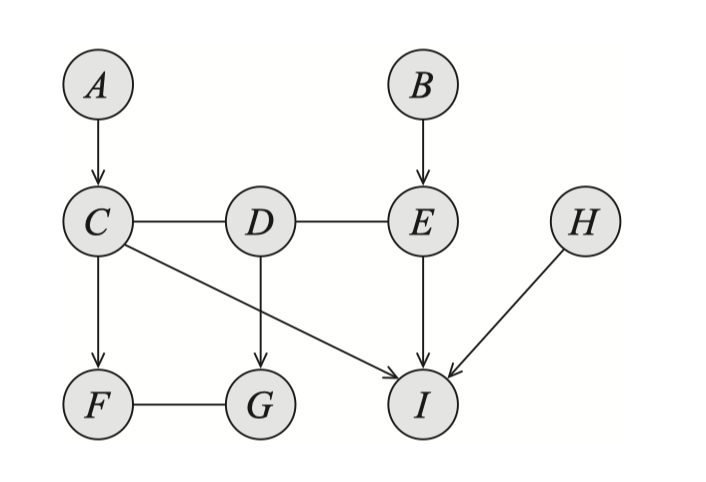
\includegraphics[width=0.4\textwidth]{Figs/a1.png}
    \caption{An example of a partially directed graph $\calK$}
    \label{fig:pa_di_gra}
\end{figure}
 We have that $A$ is the only parent of $C$, and $F, I$ are the children of $C$. The only neighbor of $C$ is $D$, but its adjacent nodes are $A, D, F, I$. 
\end{exma}
\subsection{Subgraph}
\begin{defa}\bfs{Induced Subgraph}
Let $\mathcal{K}=(\mathcal{X}, \mathcal{E})$, and let $\boldsymbol{X} \subset \mathcal{X} .$ We define the \tb{induced subgraph} $\mathcal{K}[\boldsymbol{X}]$ to be the graph $\left(\boldsymbol{X}, \mathcal{E}^{\prime}\right)$ where $\mathcal{E}^{\prime}$ are all the edges $X \rightleftharpoons Y \in \mathcal{E}$ such that $X, Y \in X$.
\end{defa}
\begin{defa}\bfs{Complete, Clique}
A subgraph over $\boldsymbol{X}$ is \tb{complete} if every two nodes in $\boldsymbol{X}$ are connected by some edge. The set $\boldsymbol{X}$ is often called a \tb{clique}; we say that a clique $\boldsymbol{X}$ is \tb{maximal} if for any superset of nodes $\boldsymbol{Y} \supset \boldsymbol{X}$, $\boldsymbol{Y}$ is not a clique.
\end{defa}
\begin{defa}\bfs{Upward Closed}\label{def:dnmfa}
\begin{itemize}
    \item We say that a subset of nodes $\boldsymbol{X} \in \mathcal{X}$ is \tb{upwardly closed} in $\mathcal{K}$ if, for any $X \in \boldsymbol{X}$, we have that  $\mathrm{Boundary}_{X} \subset \boldsymbol{X}$.
    \item We define the \tb{upward closure} of $\boldsymbol{X}$ to be the minimal upwardly closed subset $\boldsymbol{Y}$ that contains $\boldsymbol{X}$: in DAG, we have $\boldsymbol{Y}=\boldsymbol{X}\cup \mathrm{Ancestors}_{\boldsymbol{X}}$.
    \item  We define the \tb{upwardly closed subgraph}  of $\boldsymbol{X}$, denoted $\mathcal{K}^{+}[\boldsymbol{X}]$, to be the induced subgraph over $\boldsymbol{Y}, \mathcal{K}[\boldsymbol{Y}]$.
\end{itemize}
\end{defa}


\subsection{Paths and Trails (no direction)}
Using the basic notion of edges, we can define different types of longer-range connections in the graph.
\begin{defa}\bfs{Path}
We say that $X_{1}, \ldots, X_{k}$ form a path in the \tb{graph} $\mathcal{K}=(\mathcal{X}, \mathcal{E})$ if, for every $i=1, \ldots, k-1$, we have that either $X_{i} \rightarrow X_{i+1}$ or $X_{i}-X_{i+1}$. A path is \tb{directed if, for at least one $i$,} we have $X_{i} \rightarrow X_{i+1}$.
\end{defa}

\begin{defa}\bfs{Trail}
We say that $X_{1}, \ldots, X_{k}$ form a trail in the graph $\mathcal{K}=(\mathcal{X}, \mathcal{E})$ if, for every $i=1, \ldots, k-1$, we have that $X_{i} \rightleftharpoons X_{i+1}$.
\end{defa}
\begin{rema}Remember that:

\centerline{\tb{Trail has no direction requirement; Path has direction requirements}}

In undirected graph, trail $=$ path. Path can have no direction.
\end{rema}
\begin{exma}
In \cref{fig:pa_di_gra}, $A, C, F, G, D$ is a trail, which is not a path. 
\end{exma}
\begin{defa}\bfs{Connected}
A graph is connected if for every $X_{i}, X_{j}$ there is a \tb{trail} between $X_{i}$ and $X_{j}$.
\end{defa}


We can now define longer-range relationships in the graph.
\begin{defa}\bfs{Ancestor, Descendant}
 We say that $X$ is an \tb{ancestor} of $Y$ in $\mathcal{K}=(\mathcal{X}, \mathcal{E})$, and that $Y$ is a \tb{descendant} of $X$, if there exists a \tb{directed path} $X_{1}, \ldots, X_{k}$ with $X_{1}=X$ and $X_{k}=Y$. 
   \begin{itemize}
   \item $\mathrm{Descendants}_{X}$: $X$'s descendants,
    \item  $\mathrm{Ancestors}_{X}$: $X$'s ancestors
    \item $\mathrm{NonDescendants}_{X}$:  $\mathcal{X} - \mathrm{Descendants}_{X}$.
\end{itemize}

\end{defa}
\begin{rema}
 For a set of node $\boldsymbol{X}$, we also use the above notation e.g. $\mathrm{Ancestors}_{\boldsymbol{X}}$.
\end{rema}
\begin{defa}\bfs{Topological Ordering}\label{def:top_order}
 Let $\mathcal{G}=(\mathcal{X}, \mathcal{E})$ be a graph. An ordering of the nodes $X_{1}, \ldots, X_{n}$ is a topological ordering relative to $\mathcal{K}$ if, whenever we have $X_{i} \rightarrow X_{j} \in \mathcal{E}$, then $i<j$.
\end{defa}

\subsection{Cycles and Loops}
\subsubsection{Cycle: directed}
\begin{defa}\bfs{Cycle, Acyclic Graph}
 A \tb{cycle} in $\mathcal{K}$ is a \tb{directed path} $X_{1}, \ldots, X_{k}$ where $X_{1}=X_{k} .$ A graph is \tb{acyclic} if it contains no cycles.
\end{defa}


For most of this book, we will restrict attention to graphs that do not allow such cycles, since it is quite difficult to define a coherent probabilistic model over graphs with directed cycles.
\begin{defa}\bfs{DAG}
 A \tb{directed acyclic graph (DAG)} is one of the central concepts in this book, to represent \tb{Bayesian networks}. 
\end{defa}

\begin{defa}\bfs{PDAG}\label{def:cadfe}
 An acyclic graph containing both \tb{directed and undirected edges} is called a partially directed acyclic graph (PDAG).
\end{defa}
\begin{defa}\bfs{Chain Component}
Let $\mathcal{K}$ be a PDAG over $\mathcal{X}$.  { Let } $\boldsymbol{K}_{1}, \ldots, \boldsymbol{K}_{\ell}$ be a disjoint partition of $\mathcal{X}$ such that:
\begin{itemize}
    \item the induced subgraph over $\boldsymbol{K}_{i}$ contains \tb{no directed edges};
    \item for any pair of nodes $X \in \boldsymbol{K}_{i}$ and $Y \in \boldsymbol{K}_{j}$ for $i<j$, an edge between $X$ and $Y$ can only be a \tb{directed edge} $X \rightarrow Y$.
\end{itemize}
We then have each component $\boldsymbol{K}_{i}$ is called a \tb{chain component}.
\end{defa}
\begin{exma}
In \cref{fig:pa_di_gra}, we have six chain components: $\{A\},\{B\},\{C, D, E\},\{F, G\},\{H\}$, and $\{I\}$. This ordering of the chain components is one of several possible legal orderings.
\end{exma}
\begin{rema}
Note that
\begin{itemize}
    \item When the PDAG is an undirected graph, the entire graph forms a single chain component. 
    \item Conversely, when the PDAG is a directed graph (and therefore acyclic), each node in the graph is its own chain component.
\end{itemize}
\end{rema}

\subsubsection{Loop: undirected}

\centerline{\tb{Different from a cycle is the notion of a loop}}

\begin{defa}\bfs{Loop}
\begin{itemize}
    \item \tb{Loop:} a \tb{trail} $X_{1}, \ldots, X_{k}$ where $X_{1}=X_{k}$.
    \item \tb{Singly Connected:}  a graph that contains \tb{no loops}.
    \item  \tb{Leaf}: a node in a singly connected graph that has exactly one adjacent node.
    \item \tb{Polytree}: a singly connected \tb{directed} graph.
    \item \tb{(Undirected) Forest}: a singly connected undirected graph.
    \item \tb{(Undirected) Tree}: a connected undirected forest.
    \item \tb{(Directed) Forest:} a directed graph that each node has \tb{at most one parent}.
    \item  \tb{(Directed) Tree:} a directed forest is a tree if it is also connected.
\end{itemize}

\end{defa}
\begin{rema}\bfs{polytree vs tree}
Note that polytrees are very different from trees. For example, \cref{fig:polytree} shows a graph that is a polytree but is not a tree, because several nodes have \tb{more than one parent.} 
\end{rema}
\begin{figure}
    \centering
    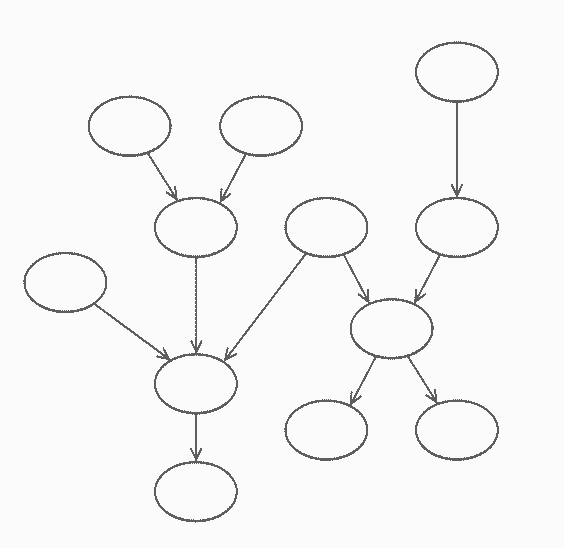
\includegraphics[width=0.4\textwidth]{Figs/a2.png}
    \caption{An example of a polytree}
    \label{fig:polytree}
\end{figure}

\begin{defa}\bfs{Chord}
Let $X_{1}-X_{2}-\cdots-X_{k}-X_{1}$ be a loop in the graph. a \tb{chord} in the loop is an edge connecting $X_{i}$ and $X_{j}$ for two \tb{nonconsecutive nodes} $X_{i}, X_{j}$. 

An \tb{undirected} graph $\mathcal{H}$ is said to be \tb{chordal} if any loop $X_{1}-X_{2}-\cdots-X_{k}-X_{1}$ for $k \geq 4$ has a chord.
\end{defa}

\begin{exma}%bfs{Triangulated}
A single loop $A-B-C-D-A$ in \cref{fig:nonchordal} is nonchordal, but adding an edge $A-C$ would render it chordal. In other words, in a chordal graph, the longest "minimal loop" (one that has no shortcut) is a triangle. Thus, chordal graphs are often also called \tb{triangulated}.
\end{exma}
\begin{figure}
    \centering
    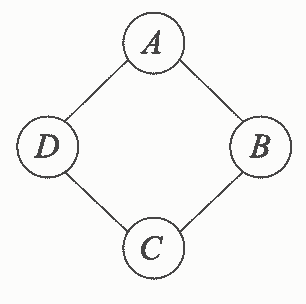
\includegraphics[width=0.4\textwidth]{Figs/a3.png}
    \caption{An example of nonchordal.}
    \label{fig:nonchordal}
\end{figure}
\begin{defa}\bfs{Extended Chord}
A graph $\mathcal{K}$ is said to be \tb{chordal} if its underlying \tb{undirected} graph is chordal.
\end{defa}
\subsection{Notations}
\begin{itemize}
    \item $\mathrm{Val}(X)$: the set of possible values of r.v. $X$.
    \item $P^{*}$ : Distribution that generated the data
\item $P \models \ldots$: $P$ satisfies ...
\item $\mathrm{~Pa}_{X}$: Parents of $X$ (in graph)
\item $\mathrm{pa}_{X}$: Value of $\mathrm{Pa}_{X}, 157$
\item $\mathrm{~Pa}_{X_{i}}^{\mathcal{G}}$: Parents of $X_{i}$ in $\mathcal{G}$
\item $\hat{P}_{\mathcal{D}}(A)$: Empirical distribution
\item $\hat{P}_{\mathcal{D}}(\boldsymbol{x})$: Empirical distribution
\item $\boldsymbol{\theta}$: Parameters
\item $\hat{\boldsymbol{\theta}}$: MLE parameters
\item $\phi$: A factor (Markov network)
\item $\boldsymbol{x}\langle\boldsymbol{Y}\rangle$: assignment in $\boldsymbol{x}$ to variables in $\boldsymbol{Y}$,
\end{itemize}




\section{The Bayesian Network Representation}

Why Baysesian network (BN)? The explicit representation of the joint distribution for large number of variables without conditional independence is unmanageable from every perspective, including computation, storage, extremely small parameters estimation, and human intuition. We need (conditional) independence to simplify the model. (Conditional) independence could be well represented using Baysesian network (DAG). That's the answer. We consider discrete randon variables in this section, however most conclusions generalize to the continuous cases or even general measures.

\subsection{Introduction}
\begin{exma}\bfs{independence parameterization}
Independent parameters are parameters whose values are not determined by others. For multinomial distribution over a $k$ dimensional space, we have $k-1$ independent parameters.

For $n$ binary valued variables, in the case where we have an arbitrary joint distribution over $n$ binary random variables, the number of independent parameters is $2^{n}-1$: $$\left\{\left(p_{1}, \ldots, p_{2^{n}}\right) \in \mathbb{R}^{2^{n}}: p_{1}+\ldots+p_{2^{n}}=1\right\}.$$ If we assume probability independence among the $n$ variables, $n$ parameters $\{\theta_1,...,\theta_n\}$ are enough:
\begin{align*}
P\left(x_{1}, \ldots, x_{n}\right)=\prod_{i} \theta_{x_{i}}.
\end{align*}
where $\theta_{x_{i}}=\theta_{i}$ when $x_{i}=x_{i}^{1}$ and $\theta_{x_{i}}=1-\theta_{i}$ when $x_{i}=x_{i}^{0}$,
\end{exma}

\begin{figure}
    \centering
    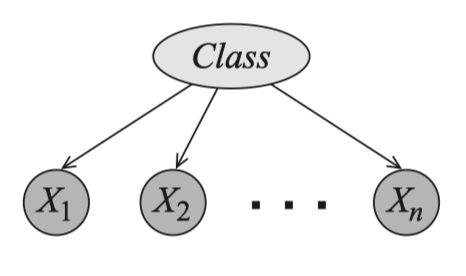
\includegraphics[width=0.4\textwidth]{Figs/a4.png}
    \caption{The Bayesian network graph for a naive Bayes model}
    \label{fig:naive_bayes}
\end{figure}

\begin{defa}\bfs{Naive Bayes Model}
 In naive Bayes model (also known as the Idiot Bayes model) we have
 \begin{enumerate}
     \item a class variable $C$ that takes on values in some set $\left\{c^{1}, \ldots, c^{k}\right\} .$
     \item some number of features $X_{1}, \ldots, X_{n}$ whose values are typically observed. The naive Bayes assumption is that the features are \tb{conditionally independent} given the instance's class.
 \end{enumerate} 
Formally, we have that
\begin{align*}
\left(X_{i} \perp \boldsymbol{X}_{-i} \mid C\right) \quad \text { for all } i,
\end{align*}
where $\boldsymbol{X}_{-i}=\left\{X_{1}, \ldots, X_{n}\right\}-\left\{X_{i}\right\} .$ 

Based on these independence assumptions, we can show that the model \tb{factorizes} as:
\begin{align*}
P\left(C, X_{1}, \ldots, X_{n}\right)=P(C) \prod_{i=1}^{n} P\left(X_{i} \mid C\right) .
\end{align*}
\end{defa}
\begin{rema}
This model can be represented using the \tb{Bayesian network} of \cref{fig:naive_bayes}. However, the exact definition of Bayesian network is deferred to \cref{sec:bay}.
\end{rema}
% \begin{rema}\bfs{explanation}
% Please note in the real word, intuitively, conditional independence statement in naive Bayes mode holds \tb{only if} the class is \tb{the only reason} why $X_i$s are correlated.

% This model can be represented using the \tb{Bayesian network} of \cref{fig:naive_bayes}.  In this model: $X_i$ depends stochastic on class $C$.

% In this example, and later on in the book, we use a \tb{darker oval} to represent variables that are always observed when the network is used. 
% \end{rema}
% \begin{rema}\bfs{generalization and principle}
% Generally speaking the models we construct often follow \tb{causal intuitions}. The edges represent  direct influence (e.g. \tb{causal dependence}) of one variable on another.
% \end{rema}
$\bullet$ \tb{Benefits of (Conditional) Independence:} 

We have two benefits:
\begin{enumerate}
    \item \tb{Reduction of parameters}: In case of binary, the number of independent parameters required to specify the distribution is $n+1$.
    \item \tb{Modularity}: we can represent the joint distribution using a small set of factors: a prior distribution $P(C)$, and a set of CPDs $P\left(X_{j} \mid C\right)$, one for each of the $n$ finding variables. When we added the new variable $G$, the joint distribution changed entirely. In the factored representation, we could reuse our local probability models for the variables.
\end{enumerate}
Please note in the real word, intuitively conditional independence statement holds \tb{only if} the class is \tb{the only reason} why $X_i$s are correlated.


\subsection{Bayesian Networks}
The core of the Bayesian network representation is a \tb{directed acyclic graph (DAG)} $\mathcal{G}$, whose nodes are the random variables in our domain and whose edges correspond, intuitively, to direct influence of one node on another. Generally speaking the models we construct often follow \tb{causal intuitions}. The edges represent  direct influence (e.g. \tb{causal dependence}) of one variable on another.

This graph $\mathcal{G}$ can be viewed in two very different ways:
\begin{itemize}
    \item  as a data structure that provides the skeleton for representing a joint distribution compactly in a factorized way;
\item  as a compact representation for a set of conditional independence assumptions about a distribution.
\end{itemize}
As we will see, these two views are, in a strong sense, equivalent:

\centerline{\tb{``factorization'' $\approx$ ``set of conditional independence''}}




\subsubsection{BN Graph Definition: Set of Local Independencies}\label{sec:bay}



\boxx{
\begin{defa}\label{def:bay_loc}\bfs{Bayesian Network Graph and Local Independencies Set $\mathcal{I}_{\ell}(\mathcal{G})$}

A Bayesian network structure $\mathcal{G}$ is a \tb{directed acyclic graph (DAG)}, where we have
\begin{itemize}
    \item Nodes: random variables $X_{1}, \ldots, X_{n} .$ 
    \item Edges: local independencies of random variables: 
    \begin{itemize}[$\diamond$]
        \item Let $\mathrm{Pa}_{X_{i}}^{\mathcal{G}}$ denote the parents of $X_{i}$ in DAG $\mathcal{G}$, and
        \item  $\mathrm{NonDescendants}_{X_{i}}$ denote the variables in the graph that are not descendants of $X_{i}$
    \end{itemize}
    
     Then $\mathcal{G}$ encodes the following set of conditional independence assumptions, called the \tb{local independencies,} and denoted by $\mathcal{I}_{\ell}(\mathcal{G})$ :
 
\centerline{\tb{``For each variable $X_{i}:\left(X_{i} \perp \mathrm{NonDescendants}_{X_{i}} \mid \mathrm{Pa}_{X_{i}}^{\mathcal{G}}\right)$.''}}

In other words, the local independencies state that \tb{each node $X_{i}$ is conditionally independent of its nondescendants given its parents.}

\end{itemize}
\end{defa}}
\begin{rema}\bfs{explanation}
Note here is a \tb{definition} for Bayesian network. That means if we put $X_i$ to each node, we \tb{have implicitly assumed the above local independencies among random variables}.
\end{rema}

\begin{exma}\bfs{Student Example} See \cref{fig:Student}.
\begin{figure}
    \centering
    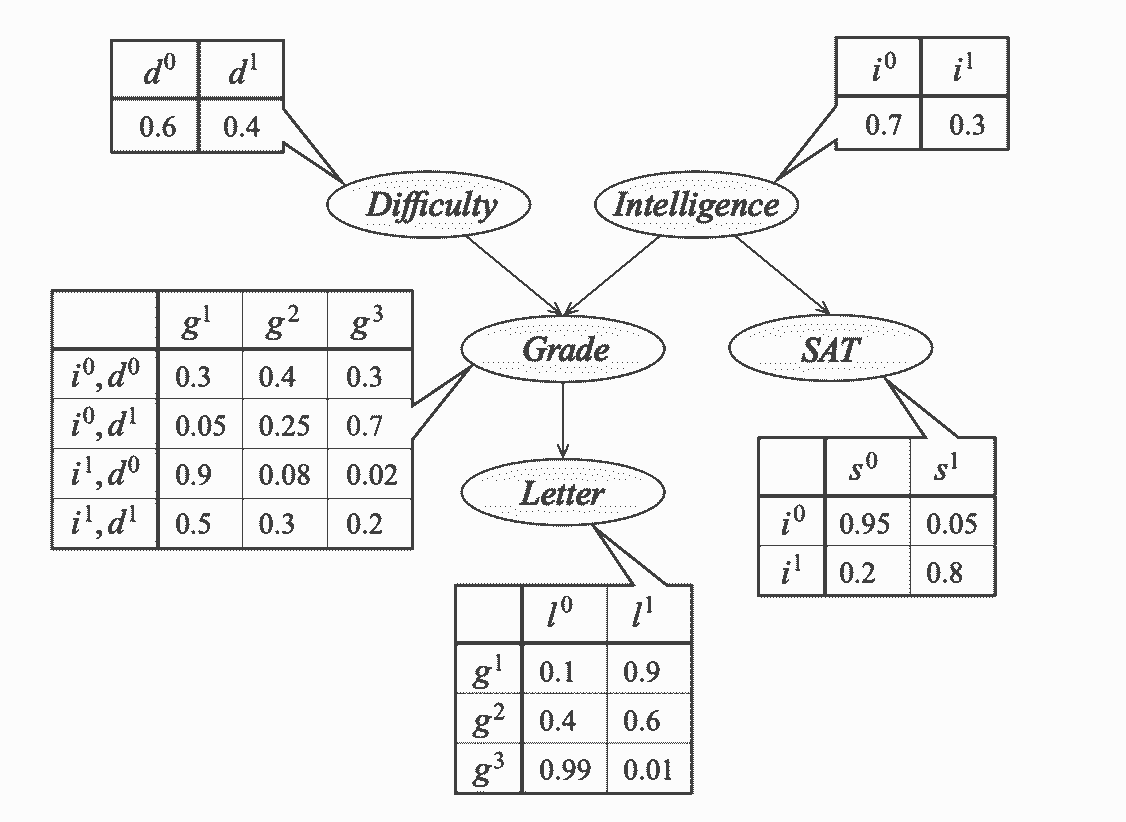
\includegraphics[width=0.8\textwidth]{Figs/a5.png}
    \caption{Student Bayesian network $\mathcal{B}^{\text {student }}$ with CPDs}
    \label{fig:Student}
\end{figure}
We have several nodes represents some  random variables with realistic meanings.
 To construct the network with those presented edges, in the following we give the intuitive explanation for the local independencies assumptions we have made.
\begin{itemize}
    \item "The professor's recommendation letter depends only on the student's grade in the class" can be stated formally as the assumption that $L$ is conditionally independent of all other nodes in the network given its parent $G$ :
\begin{align*}
(L \perp I, D, S \mid G) .
\end{align*}
\item  "Student's SAT score depends only on his intelligence", means that $S$ is conditionally independent of all other nodes in the network given its parent $I$ :
\begin{align*}
(S \perp D, G, L \mid I) .
\end{align*}
\item However $G$ is not conditionally independent of all other variables in the network given its parents.
\begin{align*}
P\left(g^{1} \mid i^{1}, d^{1}, l^{1}\right)>P\left(g^{1} \mid i^{1}, d^{1}\right) .
\end{align*}
\item "Once we know the student's grade, our beliefs about the quality of his recommendation letter are not influenced by information about any other variable", means
\begin{align*}
(G \perp S \mid I, D)
\end{align*}
\item We assumed that Intelligence and Difficulty are independent:
$(I \perp D) .$
However, we  have dependence of $I$ and $D$ given $G$: learning something about the course difficulty drastically changed our beliefs about the student’s intelligence. 
\item 
For the variable $D$, both $I$ and $S$ are nondescendants. The variable $S$ increases our beliefs in the student's intelligence, but knowing that the student is smart (or not) does not influence our beliefs in the difficulty of the course. Thus, we have that
$$(D \perp I, S)$$
\end{itemize}

\tb{In sum}, each variable is a stochastic function of its parents. Once I know the value of the parents, no information relating directly or indirectly to its parents or other ancestors can influence the beliefs about it. However, information about its descendants can change my beliefs about it, via an \tb{evidential reasoning process.}
\end{exma}



\subsubsection{Local Independencies $=$ Factorization}
 In this section, we show that a distribution $P$ satisfies the local independencies associated with a graph $\mathcal{G}$ if and only if $P$ is representable  (factorizable) as a set of CPDs associated with the graph $\mathcal{G}$. We begin by formalizing the basic concepts.
\paragraph{I-Maps}
We first define the set of independencies associated with a distribution $P$.
\begin{defa}\bfs{Set of Independence of Distribution}\label{def:fasdfer}
Let $P$ be a distribution over $\mathcal{X}$. We define $\mathcal{I}(P)$ to be the set of all independence assertions of the form $(\boldsymbol{X} \perp \boldsymbol{Y} \mid \boldsymbol{Z})$ that hold in $P$. 
\end{defa}
\begin{defa}\bfs{I-map: local independencies}
Let $\mathcal{G}$ be any DAG  associated with a set of independencies $\mathcal{I}_{\ell}(\mathcal{G}) .$ We say that $\mathcal{G}$ is an \tb{I-map} for a set of independencies $\mathcal{I}$ if $\mathcal{I}_{\ell}(\mathcal{G}) \subseteq \mathcal{I}$.%$\mathcal{I}(\mathcal{K}) \subseteq \mathcal{I}$.
\end{defa}
\begin{defa}\bfs{I-map: global independencies}\label{def:Imapglobal}
Let $\mathcal{I}(\mathcal{K})$ be the set of all independencies associated with (any type) graph $\mathcal{K}$. We say that $\mathcal{K}$ is an \tb{I-map} for a set of independencies $\mathcal{I}$ if $\mathcal{I}(\mathcal{K}) \subseteq \mathcal{I}$.%$\mathcal{I}(\mathcal{K}) \subseteq \mathcal{I}$.
\end{defa}
\begin{rema}\bfs{important reminder}
 Note so far we only can definite I-map w.r.t. the local independencies of the graph $\calG$. However, \tb{normally I-map is defined in term of global independencies} contained in the graph $\calK$. Under Bayesian network, same local independencies implies  same global independencies as shown in \cref{sec:madnffe}. However, under Markov network, they are only equivalent under positive distribution assumption. In general we use the global independencies definition.
\end{rema}
\begin{defa}\bfs{I-map for Distribution}
$\mathcal{G}$ is an \tb{I-map for $P$} if $\mathcal{G}$ is an I-map for $\mathcal{I}(P)$, i.e. if $P$ satisfies the local independencies associated with $\mathcal{G}$: $\mathcal{I}_{\ell}(\mathcal{G}) \subseteq \mathcal{I}(P)$
\end{defa}
\begin{rema}\bfs{converse is not true}\label{re:fgrer}
Any independence that $\mathcal{G}$ asserts must also hold in $P$. Conversely, $P$ may have additional independencies that are not reflected in $\mathcal{G}$. For example, all DAG are I-map for the distribution with the marginal independent  random variables. However, some independence can not be deduced from all graphs except the one with each isolated nodes.
\end{rema}

\paragraph{I-Map to Factorization}
\begin{defa}\bfs{Factorization}
Let $\mathcal{G}$ be a BN graph over the variables $X_{1}, \ldots, X_{n}$. We say that a distribution $P$ over the same space \tb{factorizes according to $\mathcal{G}$} if $P$ can be expressed as a product
\begin{align*}
P\left(X_{1}, \ldots, X_{n}\right)=\prod_{i=1}^{n} P\left(X_{i} \mid \mathrm{Pa}_{X_{i}}^{\mathcal{G}}\right) .
\end{align*}
This equation is also called the \tb{chain rule for Bayesian networks}. The individual factors $P\left(X_{i} \mid \mathrm{Pa}_{X_{i}}^{\mathcal{G}}\right)$ are called conditional probability distributions (CPDs) or local probabilistic models.
\end{defa}

\begin{thma}\bfs{I-Map to Factorization}\label{thm:imap2frac}
Let $\mathcal{G}$ { be a } BN structure over a set of random variables $\mathcal{X}$, and let $P$ { be a joint distribution over } the same space. If $\mathcal{G}$ is an I-map for $P$, then $P$ factorizes according to $\mathcal{G}$.
\end{thma}

\begin{proof}
Assume, without loss of generality, that $X_{1}, \ldots, X_{n}$ is a topological ordering of the variables in $\mathcal{X}$ relative to $\mathcal{G}$ (see \cref{def:top_order}). We first use the chain rule for probabilities:
\begin{align}
P\left(X_{1}, \ldots, X_{n}\right)=\prod_{i=1}^{n} P\left(X_{i} \mid X_{1}, \ldots, X_{i-1}\right) \label{eq:opoirdsa}.
\end{align}
Now, consider one of the factors $P\left(X_{i} \mid X_{1}, \ldots, X_{i-1}\right)$. As $\mathcal{G}$ is an I-map for $P$, we have that $\left(X_{i} \perp \mathrm{NonDescendants}_{X_{i}} \mid \mathrm{Pa}_{X_{i}}^{\mathcal{G}}\right) \in \mathcal{I}(P)$. By assumption, all of $X_{i}$'s parents are in the set $\{X_{1}, \ldots, X_{i-1}\}$. Furthermore, none of $X_{i}$'s descendants can possibly be in this set. Hence,
\begin{align*}
\left\{X_{1}, \ldots, X_{i-1}\right\}=\operatorname{Pa}_{X_{i}} \cup \boldsymbol{Z}
\end{align*}
where $\boldsymbol{Z} \subseteq$ NonDescendants $_{X_{i}} .$ From the local independencies for $X_{i}$ and from the decomposition property (see "Basic Graphical Models Notes") it follows that $\left(X_{i} \perp \boldsymbol{Z} \mid \mathrm{Pa}_{X_{i}}\right)$. Hence, we have that
\begin{align*}
P\left(X_{i} \mid X_{1}, \ldots, X_{i-1}\right)=P\left(X_{i} \mid \mathrm{Pa}_{X_{i}}\right) .
\end{align*}
Applying this transformation to all of the factors in the chain rule decomposition, the result follows.
\end{proof}
\begin{rema}
The proof is constructive, providing a precise algorithm for constructing the factorization given the distribution $P$ and the graph $\calG$.
\end{rema}


\paragraph{Factorization to I-Map}
\cref{thm:imap2frac} shows one direction of the fundamental connection between the conditional independencies encoded by the BN structure and the factorization of the distribution into local probability models: that the conditional independencies imply factorization. The converse also holds: factorization according to $\mathcal{G}$ implies the associated conditional independencies.
\begin{thma}\bfs{Factorization to I-Map}\label{thm:frac2imap}
Let $\mathcal{G}$ be a BN structure over a set of random variables $\mathcal{X}$ and let $P$ be a joint distribution over the same space. If $P$ factorizes according to $\mathcal{G}$, then $\mathcal{G}$ is an I-map for $P$.
\end{thma}
\begin{proof}
% We keep a set initialized with $S_0 = \{X_{1}, \ldots, X_{n}\}$.%
We still set  $\{X_{1}, \ldots, X_{n}\}$ as a topological ordering of the variables in $\mathcal{X}$ relative to $\mathcal{G}$ (see \cref{def:top_order}). %However, we assume the ordering is not a fixed one. Instead, for $X_i$, we can assume we have a topological ordering  with all $\mathrm{NonDescendants}_{X_{i}}$ residing on the left of $X_i$.

For $X_k$, we perform the marginalization for $X_w$ \tb{sequentially} from $w=n$ to $w=k+1$ only if $X_w$ is a \tb{descendants} of  $X_k$. We denote the sequence for $X_k$ as $S_k$. Note, $\mathrm{NonDescendants}_{X_{k}}$ is not in the marginalization because we have DAG without loop.
We then have 
    \begin{align*}
        P\left(X_{k} \mid \mathrm{Pa}_{X_{k}}^{\mathcal{G}}, \mathrm{NonDescendants}_{X_{k}}\right) & = \frac{P\bigg(\{X_k\}\cup\mathrm{Pa}_{X_{k}}^{\mathcal{G}}\cup \mathrm{NonDescendants}_{X_{k}}\bigg)}{P\bigg(\mathrm{Pa}_{X_{k}}^{\mathcal{G}}\cup \mathrm{NonDescendants}_{X_{k}}\bigg)}\\
        & = \frac{\sum_{i\in S_k} \prod_{i=1}^{n} P\left(X_{i} \mid \mathrm{Pa}_{X_{i}}^{\mathcal{G}}\right)}{\sum_{i\in S_k\cup\{k\}}\prod_{i=1}^{n} P\left(X_{i} \mid \mathrm{Pa}_{X_{i}}^{\mathcal{G}}\right)}\\
        & =  P\left(X_{k} \mid \mathrm{Pa}_{X_{k}}^{\mathcal{G}}\right)
    \end{align*}



% We have 
% \begin{align*}
% P\left(X_{1}, \ldots, X_{n}\right)&=\prod_{i=1}^{n} P\left(X_{i} \mid \mathrm{Pa}_{X_{i}}^{\mathcal{G}}\right)\\
% &=  P\left(X_{1}, \ldots, X_{k}\right) \prod_{i=k+1}^{n} P\left(X_{i} \mid \mathrm{Pa}_{X_{i}}^{\mathcal{G}}\right)\\
% \end{align*}
% We need to prove {\tb{``for each variable $X_{i}:\left(X_{i} \perp \mathrm{NonDescendants}_{X_{i}} \mid \mathrm{Pa}_{X_{i}}^{\mathcal{G}}\right)$.''}}
\end{proof}

\paragraph{Summary: Bayesian Network Definition}
We starts from the perspective that the BN graph (a DAG) encodes a set of conditional independence assumptions (I-map).
From the previous two theorems,\cref{thm:imap2frac} and \cref{thm:frac2imap}, we then have get the equivalence between I-map and factorization: 
\begin{enumerate}
    \item \tb{If a distribution $P$ satisfies the local conditional independencies of a DAG $\calG$, it imply $P$ could be factorized according to $\calG$}
    \item \tb{If we have a $P$ with factorization according to  DAG $\calG$, we can say that $P$ satisfies all the local conditional independencies of a DAG.}
\end{enumerate}
We now formally define the Bayesian network as a DAG and a corresponding distribution. 
\begin{defa}\bfs{Bayesian Network}
A Bayesian network is a pair $\mathcal{B}=(\mathcal{G}, P)$ where $P$ factorizes over $\mathcal{G}$, and where $P$ is specified as a set of CPDs associated with $\mathcal{G}$'s nodes. The distribution $P$ is often annotated $P_{\mathcal{B}}$.
\end{defa}



\subsubsection{Reasoning Patterns}
This section works as an supplemantary and is not that related to the topic of Bayesian here.
\begin{enumerate}
    \item \tb{causal reasoning:} Queries where we predict the “downstream” effects of various factors are \tb{causal reasoning or prediction.}
    \item \tb{evidential reasoning:} Queries where we reason from effects to causes, are \tb{evidential reasoning or explanation.}
    \item \tb{intercausal reasoning:}  In the reasoning pattern called intercausal reasoning, different causes of the same effect can interact.  
\end{enumerate}
\begin{exma}\bfs{Student Example} See \cref{fig:Student}. \label{ex:ndfwe}\begin{enumerate}
    \item \tb{causal reasoning:}  If we know George is not so intelligent $\left(i^{0}\right)$; and  ClassA is an easy class $\left(d^{0}\right)$. The probability that George gets a strong letter from the professor is now $P_{\mathcal{B}^{\text {student }}}\left(l^{1} \mid i^{0}, d^{0}\right) \approx 0.513$.
    \item \tb{evidential reasoning:} The probability that George has high intelligence given grade $g^3$ and SAT $s^0$:  $P_{\mathcal{B}^{\text {student }}}\left(i^{1} \mid g^{3}, s^{1}\right) \approx 0.578$.
    \item \tb{intercausal reasoning:} If George gets a $g^2$ in ClassA , we have that $P_{\mathcal{B}^{\text {student }}}\left(i^{1} \mid\right.$ $\left.g^{2}\right) \approx 0.175 .$ On the other hand, if ClassA is a hard class, we get $P_{\mathcal{B}^{\text {student }}}\left(i^{1} \mid g^{2}, d^{1}\right) \approx 0.34 .$ In effect we have \tb{explained away} the poor grade via the difficulty of the class.  Explaining away is an instance of \tb{intercausal reasoning.} 
\end{enumerate}
\end{exma}
\begin{rema}
Explaining away, however, is not the only form of intercausal reasoning. The influence can go in any direction.
\end{rema}


\subsection{Independencies in Graphs}\label{sec:ind_gra_bayes}
Dependencies and independencies are key properties of a distribution and are crucial for understanding its behavior. As we will see, independence properties can be exploited to reduce substantially the computation cost of inference.

% \cref{def:fasdfer} $\mathcal{I}(P)$ to be the set of all independence assertions of the form $(\boldsymbol{X} \perp \boldsymbol{Y} \mid \boldsymbol{Z})$ that hold in $P$, while we use $\mathcal{I}_{\ell}(\mathcal{G}).$

We need to answer \tb{``are there other independencies that hold for \tb{every} distribution $P$ that factorizes over $\mathcal{G}$?''} Note, the answer is generally yes, since $\mathcal{I}_{\ell}(\mathcal{G})\subseteq \mathcal{I}(\mathcal{G})$.
\subsubsection{D-separation}
When it is possible that $\boldsymbol{X}$ can influence $\boldsymbol{Y}$ given $\boldsymbol{Z}$, we can construct examples where this influence occurs and $(\boldsymbol{X} \perp \boldsymbol{Y} \mid \boldsymbol{Z})$ cannot hold for all of the distributions that factorize over $\mathcal{G}$. We therefore study the basic elements shown in the BN graph.

\begin{enumerate}
    \item \tb{Direct connection:} When $X$ and $Y$ are directly connected via an edge, say $X \rightarrow Y$, it is possible to construct a distribution where $X$ and $Y$ are \tb{correlated} regardless of any evidence about any of the other variables in the network. Assume $\mathrm{Val}(X)=\mathrm{Val}(Y)$; we can simply set $X=Y$ with uniformly distributed $X$ independently  of all others.
    \item \tb{Indirect connection:} It is enough to consider the four cases of a three-node network,  $X \rightleftharpoons Z \rightleftharpoons Y$,  as shown in \cref{fig:3node}.
    \begin{enumerate}
        \item \tb{Causal trail $X \rightarrow Z \rightarrow Y$ :} $X$ can influence $Y$ via $Z$ (active\footnote{When influence can flow from $X$ to $Y$ via $Z$, we say that the trail $X \rightleftharpoons Z \rightleftharpoons Y$ is \tb{active}.}) if and only if $Z$ is not observed.
        \item \tb{Evidential trail $X \leftarrow Z \leftarrow Y$ :} $X$ can influence $Y$ via $Z$ (active)  if and only if $Z$ is not observed.
        \item \tb{Common cause $X \leftarrow Z \rightarrow Y$ :} $X$ can influence $Y$ via $Z$ (active)  if and only if $Z$ is not observed.
        \item \tb{Common effect $X \rightarrow Z \leftarrow Y$ :} $X$ can influence $Y$ via $Z$ (active)  if and only if \tb{either $Z$ or one of $Z$'s descendants is observed}.

% It is useful to view probabilistic influence as a flow in the graph. Our analysis here tells us when influence from $X$ can "flow" through $Z$ to affect our beliefs about $Y$.
    \end{enumerate}
\end{enumerate}
\begin{rema}
It is useful to \tb{view probabilistic influence as a flow in the graph.} Our analysis here tells us when influence from $X$ can "flow" through $Z$ to affect our beliefs about $Y$.
\end{rema}



\begin{figure}
    \centering
    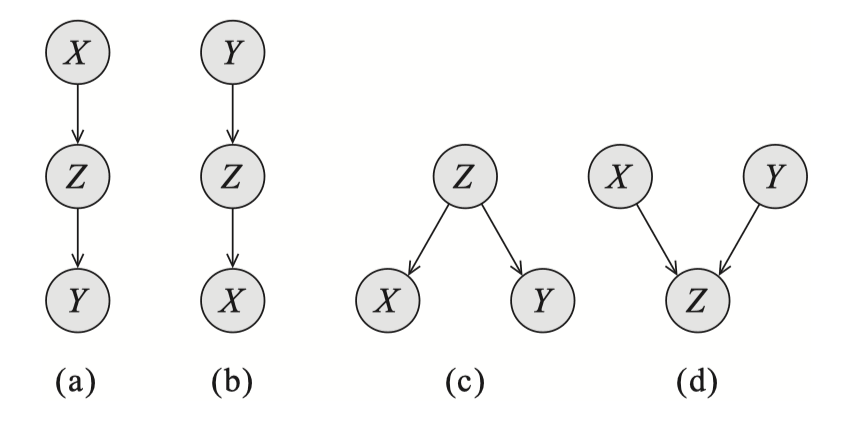
\includegraphics[width=0.6\textwidth]{Figs/a6.png}
    \caption{The four possible two-edge trails from $X$ to $Y$ via $Z$ : (a) An indirect causal effect; (b) An indirect evidential effect; (c) A common cause; (d) A common effect.}
    \label{fig:3node}
\end{figure}
\begin{defa}\bfs{$v$-structure}
A structure where $X \rightarrow Z \leftarrow Y$ (as in \cref{fig:3node} (d) ) is also called a \tb{$v$-structure}.
\end{defa}
\begin{exma}
    In \cref{ex:ndfwe}, we have \tb{explained away} the poor grade via the difficulty of the class as an instance of \tb{intercausal reasoning.} Therefore given Grade $G$, Intelligence $I$ and course Difficulty $D$  are correlated.
Without  $G$,  then $I$ and  $D$ is independent. This is an example of \tb{$v$-structure}. Also note that assume $G$ is not observed while the Letter $L$ is observer, $G$, as an descendant of $G$, can work similar as $G$ to affect $I$ and $D$.
\end{exma}


$\bullet$ \tb{General Case:}



 Now consider the case of a longer trail $X_{1} \rightleftharpoons \cdots \rightleftharpoons X_{n}$. Intuitively, for influence to "flow" from $X_{1}$ to $X_{n}$, it needs to flow through every single node on the trail. In other words, $X_{1}$ can influence $X_{n}$ if every two-edge trail $X_{i-1} \rightleftharpoons X_{i} \rightleftharpoons X_{i+1}$ along the trail allows influence to flow.
 
\begin{defa}\bfs{Trail Activeness}
Let $\mathcal{G}$ be a BN structure, and $X_{1} \rightleftharpoons \ldots \rightleftharpoons X_{n}$ a trail in $\mathcal{G}$. Let $\boldsymbol{Z}$ be a subset of observed variables. The trail $X_{1} \rightleftharpoons \ldots \rightleftharpoons X_{n}$ is \tb{active} given $\boldsymbol{Z}$ if
\begin{itemize}
    \item Whenever we have a $v$-structure $X_{i-1} \rightarrow X_{i} \leftarrow X_{i+1}$, then \tb{$X_{i}$ or one of its descendants} are in $\boldsymbol{Z}$;
    \item no other node along the trail is in $\boldsymbol{Z}$.
\end{itemize}
We also assume if $X_{1}$ or $X_{n}$ are in $\boldsymbol{Z}$ the trail is not active, since if either of them if observed, the influence is corrupted.
\end{defa}
\begin{rema}\label{re:faracvc}
Note,  a trail is not active \tb{does not imply} $X_1$ and $X_2$ are conditionally independent given $\boldsymbol{Z}$ since there may exist other trails that gives activeness (dependence). The d-separation concept below that enumerated over all possible trial is the right answer to give  conditionally independence.
\end{rema}

If there is more than one trail between two nodes, our flow intuition continues to carry through: one node can influence another if there is \tb{any} trail along which influence can flow.

\begin{defa}\bfs{Global Markov Independencies and  d-separation} 
\begin{itemize}
\item Any variables $X_{i}$ and $X_{j}$ for which $\nexists$ active trail for observations $\boldsymbol{Z}$ are called \tb{d-separated} by $\boldsymbol{Z}$. We write $\mathrm{d}$-$\mathrm{sep}\left(X_{i} ; X_{j} \mid \bZ \right)$
    \item Let $\boldsymbol{X}, \boldsymbol{Y}, \boldsymbol{Z}$ be three sets of nodes in $\mathcal{G}$. We say that $\boldsymbol{X}$ and $\boldsymbol{Y}$ are \tb{d-separated} given $\boldsymbol{Z}$, denoted $\mathrm{d}$-$\mathrm{sep}_{\mathcal{G}}(\boldsymbol{X} ; \boldsymbol{Y} \mid \boldsymbol{Z})$, if \tb{there is no active trail} between any node $X \in \boldsymbol{X}$ and $Y \in \boldsymbol{Y}$ given $\boldsymbol{Z}$, i.e. $\mathrm{d}$-$\mathrm{sep}\left(X ; Y \mid \bZ \right)$ for all $X\in \boldsymbol{X}$ and $Y\in \boldsymbol{Y}$.
    \item 
We use \tb{global Markov independencies set} $\mathcal{I}(\mathcal{G})$ to denote the set of independencies that correspond to d-separation:
\begin{align*}
\mathcal{I}(\mathcal{G})=\left\{(\boldsymbol{X} \perp \boldsymbol{Y} \mid \boldsymbol{Z}): \text{$\mathrm{d}$-$\mathrm{sep}$}_{\mathcal{G}}(\boldsymbol{X} ; \boldsymbol{Y} \mid \boldsymbol{Z})\right\} . \end{align*}
\end{itemize}
\end{defa}
\begin{rema}\bfs{reminder}
Our definition of \tb{d-separation} has been based on our intuitions regarding flow of influence (activeness). In \cref{thm:dsep1} we give proofs that \tb{d-separation} indeed corresponds to independencies, so here $\mathcal{I}(\mathcal{G})$ is indeed set of independencies.
\end{rema}
\begin{rema}\bfs{global Markov independency vs. local Markov independency}
\begin{enumerate}
    \item In \cref{def:bay_loc} of Bayesian network graph, we assume the graph with nodes representing random variables has \tb{local independencies set} $\mathcal{I}_{\ell}(\mathcal{G})$. Here we know $\mathcal{I}_{\ell}(\mathcal{G})\subseteq \mathcal{I}(\mathcal{G})$. 
    \item From \cref{def:fasdfer}, we define $\mathcal{I}(P)$ to be the \tb{set of all independence} assertions of the form $(\boldsymbol{X} \perp \boldsymbol{Y} \mid \boldsymbol{Z})$ that hold in $P$. This is a \tb{global} property for distribution $P$.  The similarity between the notation $\mathcal{I}(\mathcal{G})$ and our notation $\mathcal{I}(P)$ is not coincidental:  the independencies in $\mathcal{I}(\mathcal{G})$ are precisely those that are guaranteed to hold for \tb{every distribution} over $\mathcal{G}$.
    \item Note however as we will see same local independence $\calI_\ell(\calG)$ indicates same global $\calI(\calG)$:
    $$\text{\tb{same $\calI_\ell(\calG)$}}\Longleftrightarrow \text{\tb{same $\calI(\calG)$}}.$$
\end{enumerate}
\end{rema}


\subsubsection{Soundness and Completeness}


% Perhaps there is a distribution over the BN where $X$ can influence $Y$ despite the fact that all trails between them are blocked.
\paragraph{Soundness of D-separation: factorization to I-map}
Soundness of d-separation is the generalization of \cref{thm:frac2imap} where we only consider the local independence. Here we consider the global independence set $\calI(\calG)$. 

\tb{Soundness:} If we find that two nodes $X$ and $Y$ are d-separated given some $\boldsymbol{Z}$, then we are guaranteed that they are conditionally independent given $\boldsymbol{Z}$ in \tb{any}  $P$ factorizes according to $\mathcal{G}$. In other words:

\begin{thma}\bfs{D-separation and Independence I}\label{thm:dsep1}
\\\centerline{If a distribution $P$ factorizes according to $\mathcal{G}$, then $\mathcal{I}(\mathcal{G}) \subseteq \mathcal{I}(P)$.}
\end{thma}
\begin{rema}\bfs{explanation}
It means any independence reported by d-separation is satisfied by the underlying distribution.  
\begin{enumerate}
    \item \tb{{I-Map to Factorization} theorem, \cref{thm:imap2frac}, is the converse.}
    \item \tb{Completeness is the augment (not the converse) of Soundness with additional strong conditions (all distribution) to get $\supseteq$.}
\end{enumerate}
\end{rema}
\begin{proof}
The proof of this theorem requires some additional machinery, named Hammersley-Clifford Theorem, that we introduce in \cref{thm:Hammersley}, so we defer the proof to \cref{sec:meqkdka}.
\end{proof}
\paragraph{Completeness of D-separation:}
\tb{Question:} d-separation detects all possible independencies (strong completeness)? i.e. if $P$ factorizes according to $\mathcal{G}$, do we have $\mathcal{I}(P) \subseteq \mathcal{I}(\calG)$?

\tb{Answer:} No. See \cref{re:fgrer} for the distribution with the totally marginal mutual independent random variables. We cannot have $\mathcal{I}(P) \subseteq \mathcal{I}(\calG)$ except that $\calG$ has all isolated nodes.


\tb{Weak Completeness:} If $(X \perp Y \mid \boldsymbol{Z})$ in \tb{all distributions $P$ that factorize over $\mathcal{G}$}, then {$\mathrm{d}$-$\mathrm{sep}$}$_{\mathcal{G}}(X ; Y \mid \boldsymbol{Z}) .$  In other words:
\begin{thma}\bfs{D-separation and Independence II}\label{thm:dsep2}\\
\centerline{We have $\cap_{P\in S}\mathcal{I}(P) \subseteq \mathcal{I}(\calG)$, where  $S\coloneqq \{P: P \text{ factorizes w.r.t. $\mathcal{G}$}\}$.}
\end{thma}

\begin{proof} We prove the equivalent contrapositive statement :

\emph{``If $X$ and $Y$ are not d-separated given $\boldsymbol{Z}$ in $\mathcal{G}$, then $X$ and $Y$ are dependent given $\boldsymbol{Z}$ in some distribution $P$ that factorizes over $\mathcal{G}$.''}

The proof constructs a distribution $P$ that makes $X$ and $Y$ correlated. The construction is roughly as follows. 
\begin{enumerate}
    \item As $X$ and $Y$ are not d-separated, there exists an active trail $X=U_{1}, \ldots, U_{k}=Y$ between them. We define CPDs for the variables on the trail so as to make each pair $U_{i}, U_{i+1}$ correlated: we could define a partial deterministic for all the links. We assume $U_{i+1}=0$ if and only if $U_{i}=0$. Note here we assume the same alphabet $\calX$ for all nodes, if different $\calX_s$ for different $x\in V$, here we just change $0_{\mathrm{rest}}$ to one  vector than has one specific fixed value at one specific node. For other all possible values, we assume independently uniform for all $U_{i}$.
    \item All other CPDs containing in other active path in the graph are chosen to be independently uniform, and thus the construction guarantees that influence only flows along this single path, preventing and indes where the influence of two (or more) paths cancel out.
\end{enumerate} 
\end{proof}
% $\bullet$: A conclusion: 

% We can view the completeness result as telling us that our definition of $\mathcal{I}(\mathcal{G})$ is the maximal one. For any independence assertion that is not a consequence of d-separation in $\mathcal{G}$, we can always find a counterexample distribution $P$ that factorizes over $\mathcal{G}$. In fact, this result can be strengthened significantly:
In fact, this result can be strengthened significantly:
\begin{thma}\bfs{D-separation and Independence III}\label{thm:dsep3} \\
For \tb{almost all} distributions $P$ that factorize over $\mathcal{G}$, that is, for all distributions except for a set of measure zero in the space of CPD parameterizations, we have that $\mathcal{I}(P)=\mathcal{I}(\mathcal{G})$.
\end{thma}
\begin{proof}
$\diamond$ We first prove conditional independence statement is equivalent to  a set of polynomial equalities over the set of CPD parameters:

The Bayesian network is parameterized by a set of CPD parameters of the form $\theta_{x \mid \boldsymbol{u}}$ for $X \in \mathcal{X}, \boldsymbol{U}=\mathrm{Pa}_{X}^{\mathcal{G}}, x \in \mathrm{Val}(X), \boldsymbol{u} \in \mathrm{Val}(\boldsymbol{U}) .$ %conditional independence statement of the form $(\boldsymbol{X} \perp \boldsymbol{Y} \mid \boldsymbol{Z})$ is equivalent to a set of polynomial equalities over the set of CPD parameters $\theta_{x \mid u}$.

We consider discrete distributions in this problem. Further conditional independence constraints on the joint distribution amount to constraints on the $\theta$ parameters, which we need to prove are in polynomial equality forms. Because $P( \boldsymbol{X},  \boldsymbol{Y},  \boldsymbol{Z})=\sum_{V \notin  \boldsymbol{X} \cup  \boldsymbol{Y} \cup  \boldsymbol{Z}} \prod_{V \in \mathcal{X}} \theta_{V \mid \mathrm{Pa}_{V}^{c}}$, we can obtain distributions not necessarily for child and parents, for example, $P( \boldsymbol{Z})=\sum_{V \notin  \boldsymbol{Z}} \prod_{V \in \mathcal{X}} \theta_{V \mid \mathrm{Pa}_{V}^{c}}$ and $P( \boldsymbol{X},  \boldsymbol{Z})=\sum_{V \notin  \boldsymbol{X} \cup  \boldsymbol{Z}} \prod_{V \in \mathcal{X}} \theta_{V \mid \mathrm{Pa}_{V}^{c}}$; similar for other joint distributions over a subset of nodes in $\mathcal{B}$. We have $P( \boldsymbol{X},  \boldsymbol{Y} \mid  \boldsymbol{Z}= \boldsymbol{z})=P( \boldsymbol{X} \mid  \boldsymbol{Z}= \boldsymbol{z}) P( \boldsymbol{Y} \mid  \boldsymbol{Z}= \boldsymbol{z})$ being equivalent to
\begin{align*}
\sum_{V \notin  \boldsymbol{X} \cup  \boldsymbol{Y} \cup  \boldsymbol{Z}} \prod_{V \in \mathcal{X}} \theta_{V \mid \mathrm{Pa}_{V}^{c}} \cdot \sum_{V \notin  \boldsymbol{Z}} \prod_{V \in \mathcal{X}} \theta_{V \mid \mathrm{Pa}_{V}^{c}}=\sum_{V \notin  \boldsymbol{X} \cup  \boldsymbol{Z}} \prod_{V \in \mathcal{X}} \theta_{V \mid \mathrm{Pa}_{V}^{c}} \cdot \sum_{V \notin  \boldsymbol{Y} \cup  \boldsymbol{Z}} \prod_{V \in \mathcal{X}} \theta_{V \mid \mathrm{Pa}_{V}^{c}}
\end{align*}
a polynomial equality for $ \boldsymbol{z} \in\left\{ \boldsymbol{z}: \sum_{V \notin  \boldsymbol{Z}} \prod_{V \in \mathcal{X}} \theta_{V \mid \mathrm{Pa}_{V}^{c}} \neq 0\right\} ;$ If $P( \boldsymbol{Z}= \boldsymbol{z})=0$, we have $\left.\sum_{V \notin  \boldsymbol{Z}} \prod_{V \in \mathcal{X}} \theta_{V \mid \mathrm{Pa}_{V}^{c}}\right|_{ \boldsymbol{z}= \boldsymbol{z}}=0 .$

$\diamond$. A basic property of polynomials is that a polynomial is either identically zero or it is nonzero almost everywhere (its set of roots has measure zero). \cref{thm:dsep2}  implies that polynomials corresponding to assertions outside $\mathcal{I}(\mathcal{G})$ cannot be identically zero, because they have at least one counterexample. Thus, the set of distributions $P$, which exhibit any one of these "additional" independence assertions, has measure zero. The set of distributions that do not satisfy $\mathcal{I}(P)=\mathcal{I}(\mathcal{G})$ is the union of these separate sets, one for each additional independence assertion. The union of a countable (here is finite since there are finite many nodes and therefore finite many possible conditional independence) number of sets of measure zero is a set of measure zero, proving the result.
\end{proof}
\begin{defa}\bfs{Faithful}
A distribution $P$ is \tb{faithful} to $\mathcal{G}$ if, whenever $(X \perp Y \mid \boldsymbol{Z}) \in \mathcal{I}(P)$, then $\mathrm{d}-\operatorname{sep}_{\mathcal{G}}(X ; Y \mid \boldsymbol{Z}) .$ In other words, any independence in $P$ is reflected in the d-separation properties of the graph.
\end{defa}
From \cref{thm:dsep3}, we know \tb{almost all $P$ factorizing w.r.t. $\mathcal{G}$ is faithful.}

\paragraph{An Algorithm for D-Separation}
The notion of d-separation allows us to infer independence properties of a distribution $P$ that factorizes over $\mathcal{G}$ simply by examining the connectivity of $\mathcal{G}$. We therefore need to  determine d-separation effectively.

Instead of enumerating over all possible trails, there is a much more efficient algorithm that requires only linear time in the size of the graph. The algorithm has two phases and is presented fully in \cite[algorithm 3.1.]{koller2009probabilistic}:
\begin{enumerate}
    \item We begin by traversing the graph bottom up, from the leaves to the roots, marking all nodes that are in $\boldsymbol{Z}$ or that have descendants in $\boldsymbol{Z}$. Intuitively, these nodes will serve to enable $v$-structures.
    \item In the second phase, we traverse breadth-first from $X$ to $Y$, stopping the traversal along a trail when we get to a \tb{blocked node}. A node is \tb{blocked} if: 
    \begin{enumerate}
        \item it is the "middle" node in a $v$-structure and unmarked in phase I,
        \item is not such a node and is in $\boldsymbol{Z}$.
    \end{enumerate}
     If our breadth-first search gets us from $X$ to $Y$, then there is an active trail between them. For efficiency, and to avoid infinite loops, the algorithm must keep track of all nodes that have been visited, so as to avoid visiting them again. However, an intermediate node $Y$ might be involved in several trails, which  requires different treatment within the algorithm. See \cref{ex:drferfecd} for an example.  
\end{enumerate} 

\begin{exma}\label{ex:drferfecd}
\begin{figure}[H]
    \centering
    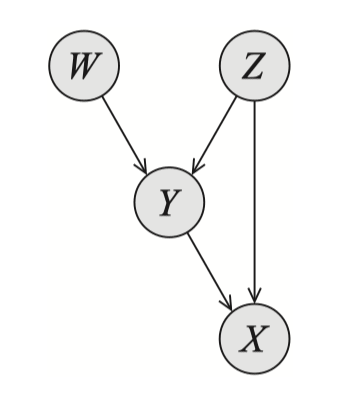
\includegraphics[width=0.2\textwidth]{Figs/a7.png}
    \caption{A simple example for the d-separation algorithm.}
    \label{fig:dsepalg}
\end{figure}
    See \cref{fig:dsepalg}. Note $Y$ may be accessed from two direction. We need to distinguish this in the algorithm.
\end{exma}

\paragraph{I-Equivalence}\label{sec:madnffe}

Very different BN structures can actually be equivalent, in that they encode precisely the same $\mathcal{I}(\mathcal{G})$, the set of conditional independence assertions.

\begin{defa}\bfs{I-Equivalence (Class)}
\begin{itemize}
    \item \tb{I-equivalence:} Two graph structures $\mathcal{K}_{1}$ and $\mathcal{K}_{2}$ over $\mathcal{X}$ are \tb{I-equivalent} if $\mathcal{I}\left(\mathcal{K}_{1}\right)=\mathcal{I}\left(\mathcal{K}_{2}\right)$. 
    \item \tb{I-equivalence class:} The set of all graphs over $\mathcal{X}$ is partitioned into a set of mutually exclusive and exhaustive I-equivalence classes, which are the \tb{set of equivalence classes induced by the I-equivalence relation}.
\end{itemize}
\end{defa}
\begin{exma}
Consider the three networks in \cref{fig:3node} (a),(b),(c). All three of them encode precisely the same independence assumptions: $(X \perp Y \mid Z)$. So they are in the same I-equivalence class. While I-equivalence class of (d) contains only (d).
\end{exma}


\begin{rema}\bfs{discussion}
\begin{enumerate}
    \item I-equivalence of two graphs immediately implies that any distribution $P$ that can be factorized over one of these graphs can be factorized over the other. Furthermore, there is no intrinsic property of $P$ that would allow us to associate it with one graph rather than an equivalent one. 
    \item \tb{How to specify the direction?} For a distribution $P(X, Y)$, whether $X$ and $Y$ are correlated, there is nothing in the distribution that can help us determine whether the correct structure is $X \rightarrow Y$ or $Y \rightarrow X$. We will return to this point when we discuss the \tb{causal interpretation} of Bayesian networks.
\end{enumerate}
\end{rema}

% The d-separation criterion allows us to using a very simple graph-based algorithm. We start by considering the trails in the networks.
\begin{defa}\bfs{Skeleton}
The \tb{skeleton} of a Bayesian network graph $\mathcal{G}$ over $\mathcal{X}$ is an undirected graph over $\mathcal{X}$ that contains an edge $\{X, Y\}$ for every edge $(X, Y)$ in $\mathcal{G}$.
\end{defa}
\begin{figure}[H]
    \centering
    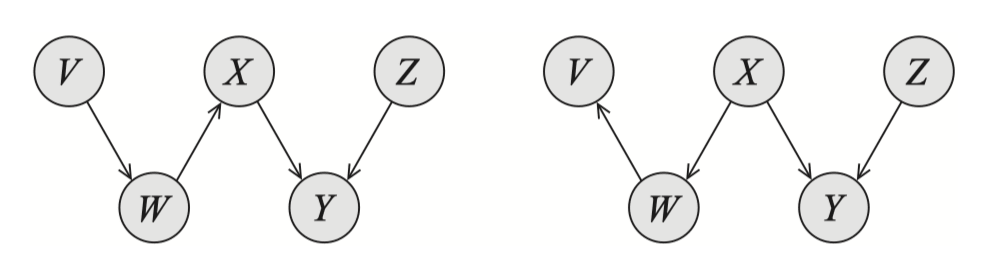
\includegraphics[width=0.5\textwidth]{Figs/a8.png}
    \caption{Skeletons and $v$-structures in a network. The two networks shown have the same skeleton and $v$-structures $(X \rightarrow Y \leftarrow Z)$.}
    \label{fig:gdazhr}
\end{figure}

\begin{exma}
In \cref{fig:gdazhr} the networks (a) and (b) have the same skeleton. 
\end{exma}
Two networks have a common skeleton is clearly not enough to conclude I-equivalence. We need the following:
\begin{thma}\bfs{skeleton + $v$-structures $\Rightarrow$ I-equivalence}
Let $\mathcal{G}_{1}$ and $\mathcal{G}_{2}$ be two graphs over $\mathcal{X}$. If $\mathcal{G}_{1}$ and $\mathcal{G}_{2}$ have the \tb{same skeleton} and the \tb{same set of $v$-structures} then they are I-equivalent.
\end{thma}

\begin{proof}
It is trivial. Since they have the same trails for all possbile $\boldsymbol{X},\boldsymbol{Y},\boldsymbol{Z}$, the same  $v$-structures further ensure one path is active in $\mathcal{G}_{1}$ if and only if it is active in  $\mathcal{G}_{2}$.
\end{proof}
\begin{rema}
\tb{Converse is not true:} There are graphs that are I-equivalent but do not have the same set of $V$-structures. As a counterexample, \tb{any two complete graphs are I-equivalent}. Although they have the same skeleton, they can have different $v$-structures.
\end{rema}
\begin{thma}\bfs{skeleton $\Leftarrow$ I-equivalence: same skeleton is necessary}
If  $\mathcal{G}_{1}$ and $\mathcal{G}_{2}$ are I-equivalence, they must have the same skeleton.
\end{thma}
\begin{proof}The principle is removing edge will adding independence.
 Suppose $X$ and $Y$ are connected in $\mathcal{G}_{1}$  but not connected in $\mathcal{G}_{2}$. The direct connection enforces $X$ and $Y$ are not independent given any other nodes. However in $\mathcal{G}_{2}$, by choosing $\boldsymbol{Z}$, we can ensure there is no active path and hence conditional independence between $X$ and $Y$.
\end{proof}
\begin{rema}We could easily show from definition that
``$\text{skeleton + same active trails}  \Longleftrightarrow \text{I-equivalence}$''.
\end{rema}

We next can provide a stronger condition that does correspond exactly to I-equivalence.

\begin{defa}\bfs{Immorality and Covering Edge}\label{def:immor}
A $v$-structure $X \rightarrow Z \leftarrow Y$ is an \tb{immorality} if there is \tb{no direct edge} between $X$ and $Y$. If there is such an edge, it is called a \tb{covering edge} for the $v$-structure.
\end{defa}
\begin{rema} Note that not every $v$-structure is an immorality, so \\
\centerline{\tb{same immorality $\centernot\implies$ same $v$-structures}}
\end{rema}

\begin{thma}\bfs{skeleton + immoralities $\Longleftrightarrow$ I-equivalence}
Let $\mathcal{G}_{1}$ and $\mathcal{G}_{2}$ be two graphs over $\mathcal{X} .$ Then $\mathcal{G}_{1}$ and $\mathcal{G}_{2}$ have the same skeleton and the same set of immoralities if and only if they are I-equivalent.
\end{thma}
\begin{proof}
See \cite[P100 ex. 3.17]{koller2009probabilistic}. Minimal active trail is the key and we first define it:

\begin{defa}\bfs{Minimal Active Trail}
Consider an active trail $T=X_{1}, X_{2}, \ldots, X_{m} .$ This active trail is called minimal if no subset of the nodes in $T$ of cardinality less than $m$ forms an active trail between $X_{1}$ and $X_{m} .$ Stated differently, $T$ is minimal if no other active trail between $X_{1}$ and $X_{m}$ "shortcuts" any of the nodes in $T$.
\end{defa}
\begin{defa}\bfs{Triangle}
Any three consecutive nodes in a trail $T=X_{1}, X_{2}, \ldots, X_{m}$ are called a triangle if their skeleton is fully connected (i.e., forms a 3-clique).
\end{defa}
$\diamond$ We first prove that ``a minimal active trail may only contain a triangle of the following form'':
\begin{itemize}[*]
    \item $X_{i-1} \leftarrow X_{i} \rightarrow X_{i+1}$
    \item $\text { Either } X_{i-1} \rightarrow X_{i+1}, \text { or } X_{i-1} \leftarrow X_{i+1}$
\end{itemize}
We need to consider 4 cases:
\begin{enumerate}
    \item $X_{i-1} \rightarrow X_{i} \rightarrow X_{i+1}$, where $X_{i}$ is unobserved. In this case, $X_{i+1} \rightarrow X_{i-1}$ will give a cycle and hence forbidden, while $X_{i-1} \rightarrow X_{i+1}$ will clearly shortcut the path since the arrow to $X_{i+1}$ are the same.
    \item $X_{i-1} \leftarrow X_{i} \leftarrow X_{i+1}$. This case is completely analogous to the previous one.
    \item $X_{i-1} \rightarrow X_{i} \leftarrow X_{i+1}$, where $X_{i}$ (or one of its children) is observed, while $X_{i-1}$ and $X_{i+1}$ can only be not observed. We only need to check whether adding an edges between $X_{i-1}$ and $X_{i+1}$ in either direction will activate a shortcut. There are 4 cases to consider, but they are all symmetric and we focus on $X_{i-1}\rightarrow X_{i+1}$: $X_{i-1} \rightarrow X_{i+1} \rightarrow X_{i+2}$ and $X_{i-1} \rightarrow X_{i+1} \leftarrow X_{i+2} .$ In the former, the shortcut is obvious; in the latter, we have a $v$-structure with $X_{i+1}$ in the middle, which is active since $X_{i}$ is observed and is a child of $X_{i+1}$.
    \item $X_{i-1} \leftarrow X_{i} \rightarrow X_{i+1}$, where $X_{i}$ is \tb{unobserved.} Similar to the above case using symmetric, we only need to focus on $X_{i-1}\rightarrow X_{i+1}$. Note the arrows to $X_{i+1}$ are the same, so we need to check $X_{i-1}$: $X_{i-2}\rightarrow X_{i-1}$ and $X_{i-2}\leftarrow X_{i-1}$. The former case render a \tb{$v$-structure} and $X_{i-1}$ should be \tb{observed}, but then $X_{i-1}\rightarrow X_{i+1}$ is not a shortcut. In the latter case $X_{i-1}$ should be unobserved, but then  $X_{i-1}\rightarrow X_{i+1}$ is a shortcut. We therefore only can choose $X_{i-2}\rightarrow X_{i-1}$.
\end{enumerate}
From the above enumeration, we can see the only possible triangles are in the case 4 and they shows the required form:  $X_{i-1} \leftarrow X_{i} \rightarrow X_{i+1}$ and $\text { either } X_{i-1} \rightarrow X_{i+1}, \text { or } X_{i-1} \leftarrow X_{i+1}$.

$\diamond$ We next prove the two equivalence:
\begin{enumerate}
    \item $\text{\tb{skeleton + immorality}} \Longleftarrow \text{\tb{I-equivalence}}$: Let $\calG_1$ and $\calG_2$ be I-equivalent. We have proved that they must have the same skeletons. We prove the fact that they have the same set of immoralities by contradiction. Assume that $\calG_1$ has an immorality, $X \rightarrow Z \leftarrow Y$, while $\calG_2$ doesn't (i.e., $X, Y, Z$ are also connected as in \cref{fig:3node} (a), (b) or (c)). Let $Z$ be unobserved, which makes $X$ and $Y$ dependent in $\calG_2$ regardless of which other nodes we condition on. In $\calG_1$, those could be either dependent or independent (as we have mentioned in \cref{re:faracvc}). Let us condition on a set of nodes, $W$, which d-separate $X$ and $Y$ ($Z \notin W$). Now, $X \perp Y \mid W$ in $\calG_1$ and $X \not \perp Y \mid W$ in $\calG_2$ which leads to a contradiction.
\item $\text{\tb{skeleton + immorality}} \Longrightarrow \text{\tb{I-equivalence}}$: Let $\calG_1$ and $\calG_2$ have the same skeletons and immoralities. Again, let's assume the contrary of the statement: $\calG_1$ and $\calG_2$ are not I-equivalent, i.e., there exit $X, Y$ and $\boldsymbol{Z}$ such that $X \perp Y \mid \boldsymbol{Z}$ in $\calG_1$ and not in $\calG_2$.
Since, by assumtion, $X \not \perp Y \mid \boldsymbol{Z}$ in $\calG_2$, completeness of d-separation implies that there should exist at least one active trail between $X$ and $Y$. Let's consider the minimal trail $t_2$ in $\calG_2$ and the corresponding trail $t_1$ in $\calG_1$.
Since $\calG_1$ and $\calG_2$ have the same skeletons, the only difference between the same trails in $\calG_1$ and $\calG_2$ is that the trail may have different directions. For the \cref{fig:3node} (a), (b) or (c) connection in both trails, given $\boldsymbol{Z}$, the activeness should not be changed. The only possible case is that the two trails have different $v$-structure. Since  $\calG_1$ and $\calG_2$ have the same immoralities. There are two possibilities: 
\begin{enumerate}
\item There exist one \tb{$v$-structure with covering edge} in the $t_2$ but not in $t_2$: This is not allowed as we have shown above since this will add a shortcut rendering $t_1$ is not  minimal. Also this means all $v$-structure in $t_2$ should be immoralities and therefore should also in $t_1$.
    \item There exist one \tb{$v$-structure with covering edge} in the $t_1$ but not in $t_2$: But then one corresponding edge should also be presented in the \tb{minimal trail} $t_2$. From the above triangle cases, we know it is only possible that  $X_{i-1} \leftarrow X_{i} \rightarrow X_{i+1}$ in $t_2$. WLOG we consider that $X_{i-1} \rightarrow X_{i+1}$ and as we have shown a \tb{$v$-structure $X_{i-2} \rightarrow X_{i-1}\leftarrow X_{i}$}  needs to be presented in $t_2$. However then $X_{i-2} \rightarrow X_{i-1}\leftarrow X_{i}$ needs to be presented in $t_1$. Now the arrow contradiction of $X_{i-1}$ in $t_1$ appears.
\end{enumerate}
\end{enumerate}
Both cases are impossible. We conclude that $v$-structures (and need to be immoralities) in $t_1$  and $t_2$ are also the same. $t_1$ must be active too if $t_1$ is the minimal trail. 
\end{proof}


We conclude with a final characterization of I-equivalence in terms of local operations on the graph structure.
\begin{defa}\bfs{Covered Edge}
An edge $X \rightarrow Y$ in a graph $\mathcal{G}$ is said to be \tb{covered} if $\mathrm{Pa}_{Y}^{\mathcal{G}}=\mathrm{Pa}_{X}^{\mathcal{G}} \cup\{X\}$.
\end{defa}
\begin{thma}
Two graphs $\mathcal{G}$ and $\mathcal{G}^{\prime}$ are I-equivalent if and only if there exists a sequence of networks $\mathcal{G}=$ $\mathcal{G}_{1}, \ldots, \mathcal{G}_{k}=\mathcal{G}^{\prime}$ that are all I-equivalent to $\mathcal{G}$ such that the only difference between $\mathcal{G}_{i}$ and $\mathcal{G}_{i+1}$ is a \tb{single reversal} of a covered edge.
\end{thma}
\begin{proof}
 Interesting but I don't have time to think how to prove.
\end{proof}

$\bullet$ \tb{Summary:}
\begin{align*}
    \text{\tb{skeleton + $v$-structures}} &\Longrightarrow \text{\tb{I-equivalence}}\\
    \text{\tb{skeleton + $v$-structures}} &\centernot\Longleftarrow \text{\tb{I-equivalence}}\\
    \text{\tb{skeleton + immorality}} &\Longleftrightarrow \text{\tb{I-equivalence}}\\
    \text{\tb{skeleton}} & \Longleftarrow \text{\tb{I-equivalence}}\\
    \text{\tb{skeleton + same active trails}} & \Longleftrightarrow \text{\tb{I-equivalence}}\\
    \text{\tb{same local independence\footnote{This is because same same local independence implies the same factorization for all possible distribution and therefore I-equivalence. I-equivalence is the global Markov set and implies the local one}}} & \Longleftrightarrow \text{\tb{I-equivalence}}\\
\end{align*}


\subsection{From Distributions to Graphs}
In the previous sections, we showed that, if $P$ factorizes over $\mathcal{G}$, we can derive a rich set of independence assertions that hold for $P$ by simply examining $\mathcal{G}$. This result immediately leads to the idea that we can use a graph as a way of revealing the structure in a distribution. 

 \tb{Question:} Given a distribution $P$, to what extent can we construct a graph $\mathcal{G}$ whose independencies are a reasonable surrogate for the independencies in $P$?

\subsubsection{Minimal I-Maps}
\begin{defa}\bfs{Minimal I-map}\label{def:nmfae}
A graph $\mathcal{K}$ is a minimal I-map for a set of independencies $\mathcal{I}$ if it is an I-map for $\mathcal{I}$, and if the removal of even a single edge from $\mathcal{K}$ renders it not an I-map.
\end{defa}
\begin{rema}\bfs{explanation}
The complete graph is an I-map for any distribution (that is representable in DAG), yet it does not reveal any of the independence structure in the distribution. However, examples such as this one are not very interesting. We therefore try to define the \tb{most representative graph} for the distribution. 
\end{rema}
\paragraph{Minimal I-map Contruction}\label{sec:jhdsddq}
 The proof of the factorization theorem \cref{thm:imap2frac} gives us a procedure, which is shown in:
\begin{figure}[H]
    \centering
    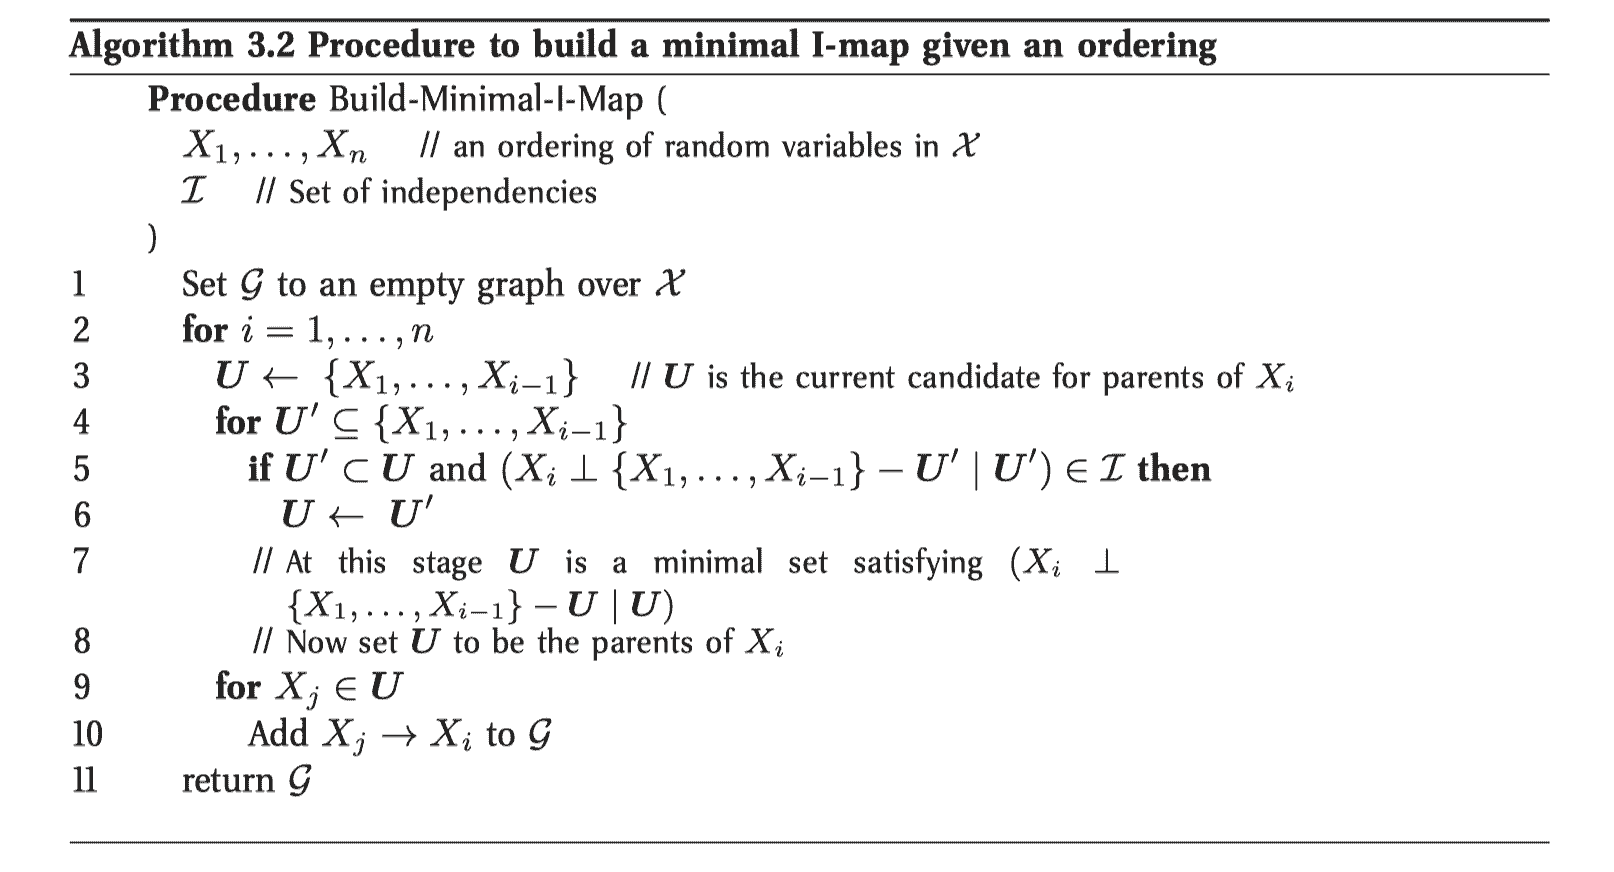
\includegraphics[width=0.8\textwidth]{Figs/a9.png}
    \caption{Procedure to build a minimal I-map given an ordering}
    \label{fig:imapminimal}
\end{figure}
\begin{enumerate}
    \item We assume we are given a predetermined variable ordering, say, $\left\{X_{1}, \ldots, X_{n}\right\}$.
    \item For each $X_{i}$, we pick some minimal subset $\boldsymbol{U}$ of $\left\{X_{1}, \ldots, X_{i-1}\right\}$ to be $X_{i}$'s parents in $\mathcal{G}$. More precisely, we require that $\boldsymbol{U}$ satisfy $\left(X_{i} \perp\left\{X_{1}, \ldots, X_{i-1}\right\}-\boldsymbol{U} \mid \boldsymbol{U}\right)$, and that no node can be removed from $\boldsymbol{U}$ without violating this property. We then set $\boldsymbol{U}$ to be the parents of $X_{i}$.
\end{enumerate}
We have then $P$ factorizes over $\mathcal{G}$ using the chain rule as shown in \cref{eq:opoirdsa}. We can then conclude from \cref{thm:frac2imap} that $\mathcal{G}$ is an I-map for $P$. By construction, $\mathcal{G}$ is minimal, so that $\mathcal{G}$ is a \tb{minimal I-map} for $P$.
\begin{rema}\bfs{uniqueness of $\boldsymbol{U}$}
Even for a given order, that our choice of $\boldsymbol{U}$ may not be unique. One can show that, if the distribution is positive, that is if for any instantiation $\xi$ to all the network variables $\mathcal{X}$ we have that $P(\xi)>0$, then the choice of parent set, \tb{given an ordering}, is unique. 
\end{rema}
\begin{exma}
But different ordering, we can get different  minimal graph, as shown in \cref{fig:ujughfa}.
\end{exma}

$\bullet$ \tb{Can we get all of the independencies in $P$ directly from minimal $\calG$? No} 

\begin{figure}[H]
    \centering
    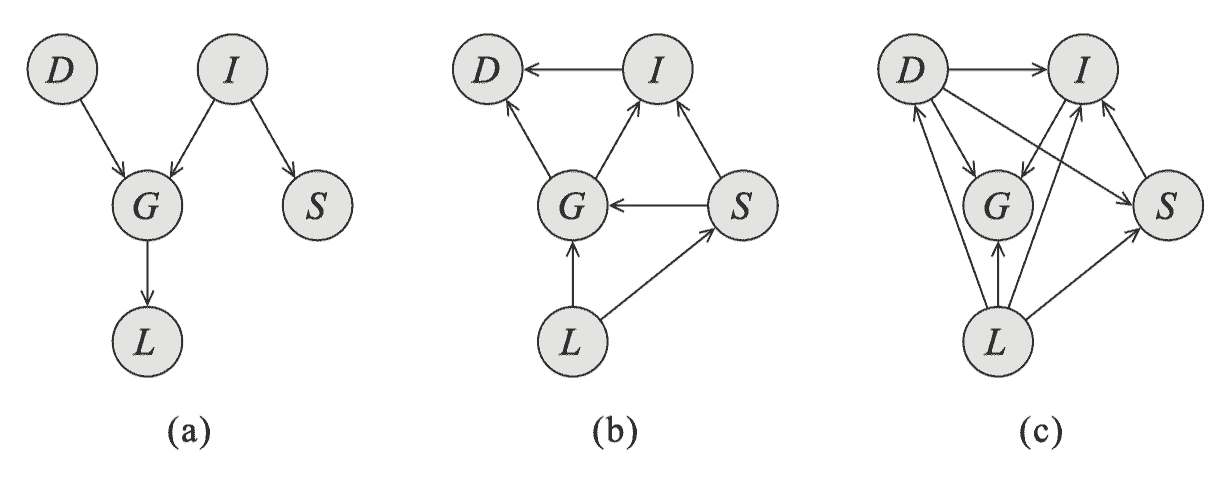
\includegraphics[width=0.8\textwidth]{Figs/a10.png}
    \caption{Three minimal I-maps for $P_{\mathcal{B}^{\text {student }}}$, induced by different orderings: (a) $D, I, S, G, L$; (b) $L, S, G, I, D$; (c) $L, D, S, I, G$.}
    \label{fig:ujughfa}
\end{figure}

\begin{exma}
Note that the graphs in \cref{fig:ujughfa} (b) and (c) really are minimal I-maps for this distribution. However, they fail to capture some or all of the independencies that hold in the distribution. Thus, they show that the fact that $\mathcal{G}$ is a minimal I-map for $P$ is far from a guarantee that $\mathcal{G}$ captures the independence structure in $P$.
\end{exma}

\subsubsection{Perfect Maps}
$\bullet$ \tb{Aim:} to find a graph $\mathcal{G}$ that precisely captures the independencies in a given distribution $P$
\begin{defa}\bfs{P-map}
We say that a graph $\mathcal{K}$ is a \tb{perfect map (P-map)} for a set of independencies $\mathcal{I}$ if we have that $\mathcal{I}(\mathcal{K})=\mathcal{I}$. We say that $\mathcal{K}$ is a perfect map for $P$ if $\mathcal{I}(\mathcal{K})=\mathcal{I}(P)$.
\end{defa}
\tb{Question:} Does every distribution has a perfect map? \tb{No.}

Not every distribution independencies can be captured by a directed graph:
\begin{itemize}
    \item Regularity in the parameterization of the distribution that cannot be captured in the graph structure, e.g., 
    \begin{exma}\bfs{XOR example}
    \begin{align*}
P(x, y, z)= \begin{cases}1 / 12 & \text { if } x \oplus y \oplus z=\text { false } \\ 1 / 6 & \text { if } x \oplus y \oplus z=\text { true }\end{cases}
\end{align*}
\begin{enumerate}
    \item $(X \perp Y) \in \mathcal{I}(P)$
    \item $Z$ is not independent of $X$ given $Y$ or $Y$ given $X$.
    \item An I-map is the network $X \rightarrow Z \leftarrow Y$.
    \item This is \tb{not a perfect map} as $(X \perp Z) \in \mathcal{I}(P)$
\end{enumerate}
    \end{exma}
\item Independence assumptions imposed by the structure of the DBN are not appropriate, e.g., \begin{exma}\bfs{Misconception example}
\label{ex:miscon}
We have that $A$ and $C$ are conditionally independent given $B$ and $D$. Similarly, $B$ and $D$ are conditionally independent given $A$ and $C$. Can we represent this distribution (with these independence properties) using a BN? One attempt is shown in \cref{fig:mfsfyuh} (b). Indeed, it encodes the independence assumption that $(A \perp C \mid\{B, D\})$. However, it also implies that $B$ and $D$ are independent given only $A$, but dependent given both $A$ and $C$. \cref{fig:mfsfyuh} (c) and all other possible BN can all be shown that they cannot correct capture the independence.
\begin{figure}[H]
    \centering
    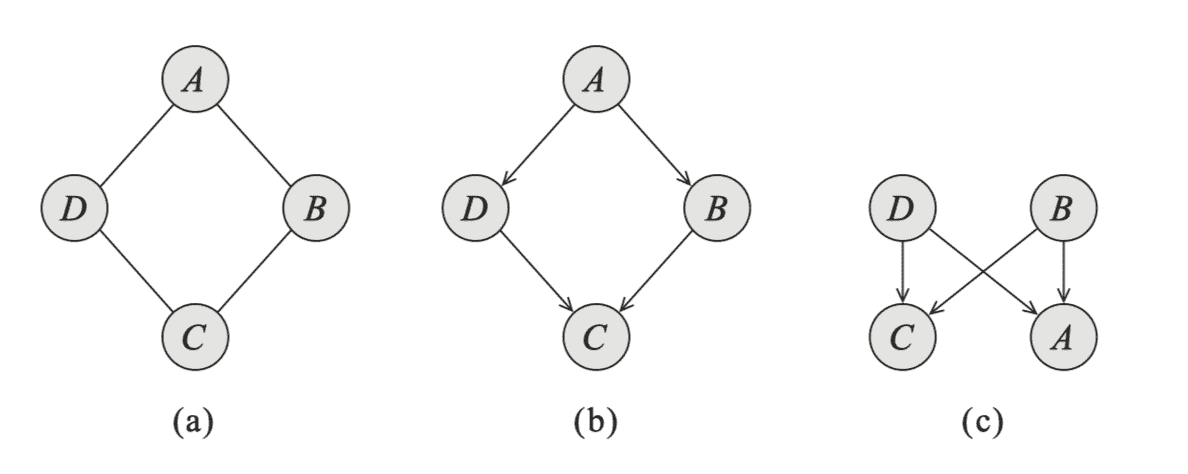
\includegraphics[width=0.8\textwidth]{Figs/a11.png}
    \caption{Attempted Bayesian network models for the Misconception example: (a) Study pairs over four students. (b) First attempt at a Bayesian network model. (c) Second attempt at a Bayesian network model.}
    \label{fig:mfsfyuh}
\end{figure}
\end{exma}

\end{itemize}

\subsubsection{Finding Perfect Maps}
Earlier we discussed an algorithm for finding minimal I-maps. We now consider an algorithm for finding a perfect map (P-map) of a distribution. Because the requirements from a P-map are stronger than the ones we require from an I-map, the algorithm will be more involved.
Perfect maps is unique up to I-equivalence between networks.
We would like to get all the perfect maps in the whole I-equivalence class by determining \tb{its skeleton and its immoralities} from the independence properties of the given distribution $P$.
\paragraph{Identifying the Undirected Skeleton}
\begin{lema}
Let $\mathcal{G}^{*}$ be a P-map of a distribution $\mathcal{P}$, and let $X$ and $Y$ be two variables such that $X \rightarrow Y$ is in $\mathcal{G}^{*}$. Then, $P \not \models(X \perp Y \mid \boldsymbol{U})$ for any set $\boldsymbol{U}$ that does not include $X$ and $Y$.
\end{lema}
\begin{proof}
 Easy.
\end{proof}
\begin{lema}
Let $\mathcal{G}^{*}$ be an I-map of a distribution $P$, and let $X$ and $Y$ be two variables that are not adjacent in $\mathcal{G}^{*}$. Then either $P \models\left(X \perp Y \mid \mathrm{Pa}_{X}^{\mathcal{G}^{*}}\right)$ or $P \models\left(X \perp Y \mid \mathrm{Pa}_{Y}^{\mathcal{G}^{*}}\right)$.
\end{lema}
\begin{proof}
 Just consider there are only two cases: $X$ is $Y$’s descendants or $Y$ is $X$’s descendant.
\end{proof}
\begin{defa}\bfs{\tb{Witness}}
Thus, if $X$ and $Y$ are not adjacent in $\mathcal{G}^{*}$, then we can find a set $\boldsymbol{U}$ so that $\mathcal{P} \models(X \perp Y \mid \boldsymbol{U})$. We call this set $\boldsymbol{U}$ a \tb{witness} of their independence.
\end{defa}
  The algorithm has two phases and is presented fully in \cite[algorithm 3.3. Build-PMap-Skeleton]{koller2009probabilistic}:
\begin{enumerate}
    \item Let $\mathcal{H}$ be the complete undirected graph over $\mathcal{X}$
\item If we can find a \tb{witness}  for $X_{i}-X_{j}$. Remove $X_{i}-X_{j}$ from $\mathcal{H}$
\end{enumerate}
\paragraph{Identifying Immoralities}
\begin{defa}\bfs{Potential Immoralities}
 A triplet of variables $X, Z, Y$ is a \tb{potential immorality} if the skeleton contains $X-Z-Y$ but does not contain an edge between $X$ and $Y$. 
\end{defa}
\tb{Goal:} consider potential immoralities in the skeleton and for each one determine whether it is indeed an immorality.

\begin{lema}
Let  $\mathcal{G}^{*}$ be a P-map of a distribution $P$,   and let $X$, $Y$ and $Z$   be variables that form an immorality  $X \rightarrow Z \leftarrow Y$. Then, $P \not \models(X \perp Y \mid \boldsymbol{U})$ for any set $\boldsymbol{U}$ that contains $Z$.
\end{lema}
\begin{lema}
Let $\mathcal{G}^{*}$ be a P-map of a distribution $P$, and let the triplet $X-Y-Z$ be a potential immorality in the skeleton of $\mathcal{G}^{*}$, such that $X \rightarrow Z \leftarrow Y$ is \tb{not} in $\mathcal{G}^{*}$ (i.e. not a immorality). If $\boldsymbol{U}$ is such that $P \models(X \perp Y \mid \boldsymbol{U})$, then $Z \in \boldsymbol{U}$.
\end{lema}
\begin{proof}
 Both easy from the four cases in \cref{fig:3node}.
\end{proof}
\begin{rema}
Combining these two results, we see that a potential immorality $X-Z-Y$ is an immorality if and only if $Z$ is \tb{not} in the witness set(s) for $X$ and $Y$.
\end{rema}
 The algorithm has two phases and is presented fully in \cite[algorithm 3.4.]{koller2009probabilistic} by checking  if $Z$ is in the witness.
 \paragraph{Representing Equivalence Classes: PDAG}
 \begin{defa}\bfs{Class PDAG}
  Let $\mathcal{G}$ be a DAG. A chain graph $\mathcal{K}$ is a class PDAG of the equivalence class of $\mathcal{G}$ if shares the same skeleton as $\mathcal{G}$, and contains a directed edge $X \rightarrow Y$ if and only if all $\mathcal{G}^{\prime}$ that are I-equivalent to $\mathcal{G}$ contain the edge $X \rightarrow Y$.
 \end{defa}
\begin{rema}\bfs{explanation}
If the edge is directed, then all the members of the equivalence class agree on the orientation of the edge. If the edge is undirected, there are two DAGs in the equivalence class that disagree on the orientation of the edge.
\end{rema}

\tb{Question:} Can $\mathcal{K}$  contain directed edges that are not involved in immoralities? \tb{Yes.}

\begin{figure}[H]
    \centering
    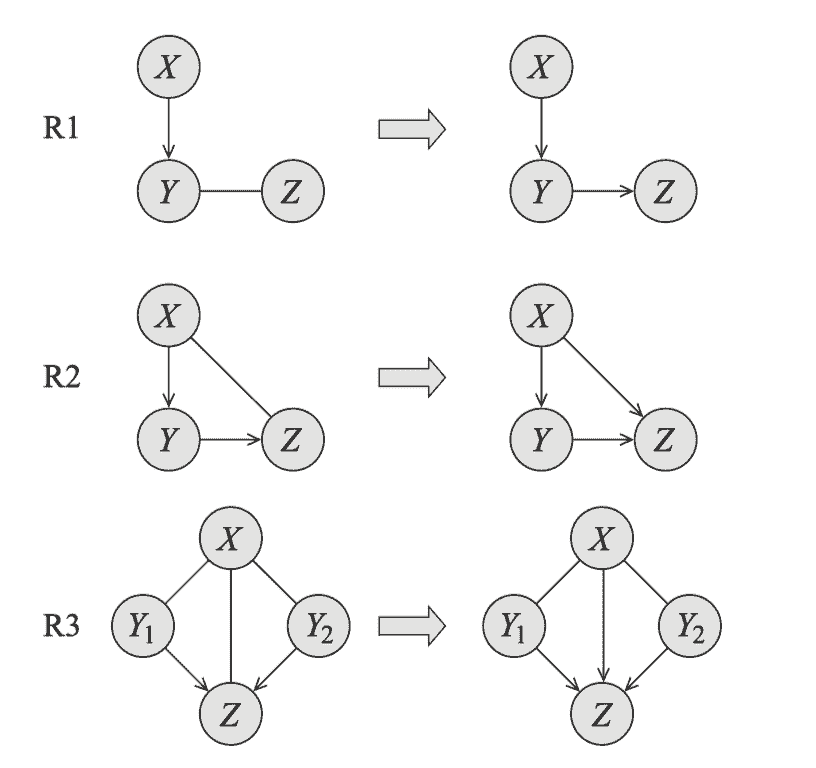
\includegraphics[width=0.4\textwidth]{Figs/a12.png}
    \caption{Rules for orienting edges in PDAG. Each rule lists a configuration of edges before and after an application of the rule.}
    \label{fig:jtrsfsd}
\end{figure}

The algorithm is presented fully in \cite[algorithm 3.5.]{koller2009probabilistic}: It builds an initial graph skeleton and immoralities, and then iteratively applies the \tb{three rules} shown in \cref{fig:jtrsfsd} until convergence.

% \begin{figure}[H]
%      \centering
%      \begin{subfigure}[b]{0.3\textwidth}
%          \centering
%          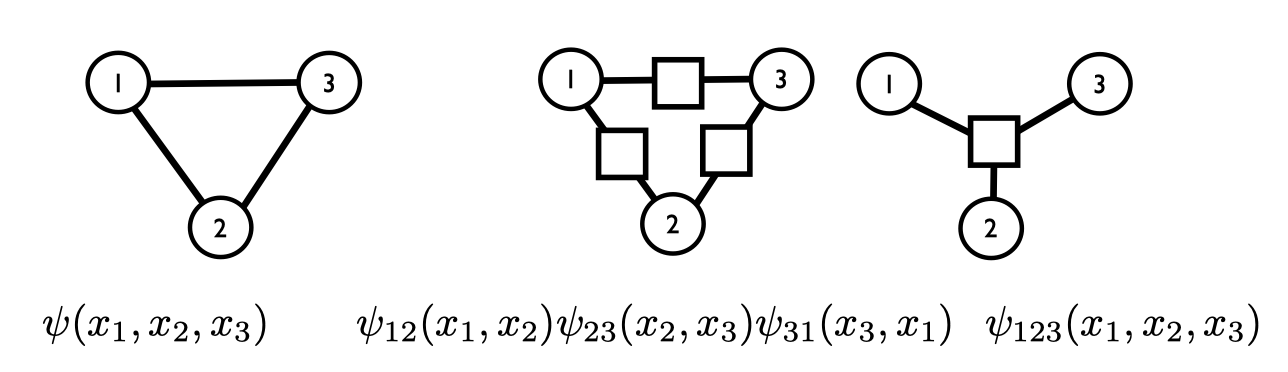
\includegraphics[width=\textwidth]{Figs/3.png}
%          \caption{function $\alpha$}
%      \end{subfigure}
%      \hfill
%      \begin{subfigure}[b]{0.47\textwidth}
%          \centering
%          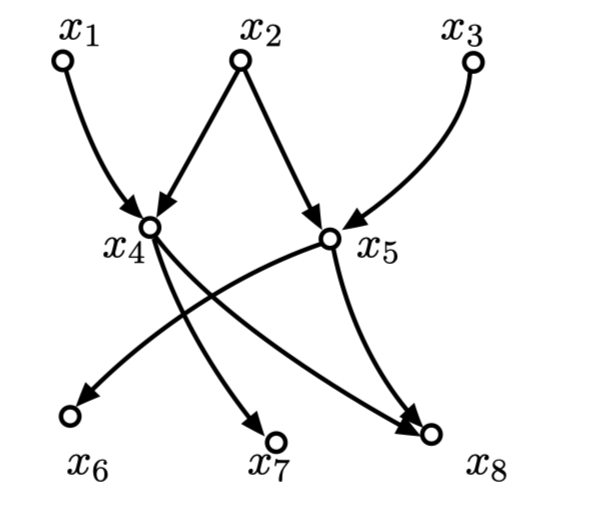
\includegraphics[width=\textwidth]{Figs/4.png}
%      \end{subfigure}
% \end{figure}
\section{Undirected Graphical Models}
Undirected graphical models are useful in random variables where we cannot naturally ascribe a directionality to the interaction between variables. Instead of CPD, sometimes we need a more symmetric parameterization. Edges correspond to a notion of direct probabilistic interaction between the neighboring variables an interaction that is not mediated by any other variable in the network. 
\begin{itemize}
    \item Undirected graphical model: better for modeling \tb{correlations} between variables.
    \item Directed graphical model: better for modeling \tb{causality} between variables.
\end{itemize}
Please read ``{Markov Property for Undirected Graphs}'' in ``Basic Graphical Models Notes''. Hammersley-Clifford Theorem and its proof are given in that section. Global, local and pairwise Markov Property are also proved in details there.
\subsection{Definitions and Parameterization}
To represent a distribution, we need to associate the graph structure with a set of parameters, in the same way that CPDs were used to parameterize the directed graph structure.
\subsubsection{Factor}
\begin{defa}\bfs{Factor, Scope}
 Let $\boldsymbol{D}$ be a set of random variables. We define a \tb{factor} $\phi$ to be a function from $\mathrm{Val}(\boldsymbol{D})$ to $\mathbb{R}^{+}$. A factor is nonnegative if all its entries are nonnegative. The set of variables $\boldsymbol{D}$ is called the \tb{scope} of the factor and denoted  $\mathrm{Scope}[\phi]$.
\end{defa}
\begin{rema}
Unless stated otherwise, we restrict attention to \tb{nonnegative} factors.
The factor value associated with a particular scope variables values assignment denotes the \tb{affinity} between them : the \tb{higher} the factor value $\phi_{1}(a, b)$, the \tb{more compatible} these two variables values are. A factor subsumes both the notion of a joint distribution and the notion of a CPD (with additional normalization constraints):
\begin{enumerate}
    \item A joint distribution over $\boldsymbol{D}$ is a factor over $\boldsymbol{D}$ : it specifies a real number for every assignment of values of $\boldsymbol{D}$.
    \item  A conditional distribution $P(X \mid \boldsymbol{U})$ is a factor over $\{X\} \cup \boldsymbol{U}$.
\end{enumerate} 
\end{rema}
\begin{defa}\bfs{Factor Product}
 Let $\boldsymbol{X}, \boldsymbol{Y}$, and $\boldsymbol{Z}$ be three disjoint sets of variables, and let $\phi_{1}(\boldsymbol{X}, \boldsymbol{Y})$ and $\phi_{2}(\boldsymbol{Y}, \boldsymbol{Z})$ be two factors. We define the factor product $\phi_{1} \times \phi_{2}$ to be a factor $\psi: \mathrm{Val}(\boldsymbol{X}, \boldsymbol{Y}, \boldsymbol{Z}) \mapsto \mathbb{R}$ as follows:
\begin{align*}
\psi(\boldsymbol{X}, \boldsymbol{Y}, \boldsymbol{Z})=\phi_{1}(\boldsymbol{X}, \boldsymbol{Y}) \cdot \phi_{2}(\boldsymbol{Y}, \boldsymbol{Z}) .
\end{align*}
\end{defa}
\begin{rema}\bfs{factor bayesian network}
letting $\phi_{X_{i}}\left(X_{i}, \mathrm{Pa}_{X_{i}}\right)$ represent $P\left(X_{i} \mid \mathrm{Pa}_{X_{i}}\right)$, we have that
\begin{align*}
P\left(X_{1}, \ldots, X_{n}\right)=\prod_{i} \phi_{X_{i}}
\end{align*}
\end{rema}
\subsubsection{Gibbs Distributions and Markov Networks}
We can now use the more general notion of factor product to define an undirected parameterization of a distribution.
\begin{defa}\bfs{Gibbs distribution, Partition Function}\label{def:xzda}
 A distribution $P_{\Phi}$ is a \tb{Gibbs distribution parameterized by a set of factors} $\Phi=\left\{\phi_{1}\left(\boldsymbol{D}_{1}\right), \ldots, \phi_{K}\left(\boldsymbol{D}_{K}\right)\right\}$ if it is defined as follows:
\begin{align}
P_{\Phi}\left(X_{1}, \ldots, X_{n}\right)=\frac{1}{Z} \tilde{P}_{\Phi}\left(X_{1}, \ldots, X_{n}\right)\label{eq:jeaxc}
\end{align}
where
\begin{align*}
\tilde{P}_{\Phi}\left(X_{1}, \ldots, X_{n}\right)=\phi_{1}\left(\boldsymbol{D}_{1}\right) \times \phi_{2}\left(\boldsymbol{D}_{2}\right) \times \cdots \times \phi_{m}\left(\boldsymbol{D}_{m}\right)
\end{align*}
is an unnormalized measure and
\begin{align*}
Z=\sum_{X_{1}, \ldots, X_{n}} \tilde{P}_{\Phi}\left(X_{1}, \ldots, X_{n}\right)
\end{align*}
is a normalizing constant called the \tb{partition function}.
\end{defa}
\tb{Question:}  How to relate the parameterization of a Gibbs distribution to a graph structure?

If the parameterization contains a factor whose scope contains $X$ and $Y$, we introduce a direct interaction between them and want one edge between $X$ and $Y$ in the graph to denote the interaction.
\begin{defa}\bfs{Markov Network Factorization}\label{def:Markov_fac}
 We say that a distribution $P_{\Phi}$ with $\Phi=\left\{\phi_{1}\left(\boldsymbol{D}_{1}\right), \ldots, \phi_{K}\left(\boldsymbol{D}_{K}\right)\right\}$ factorizes over a Markov network $\mathcal{H}$ if each $\boldsymbol{D}_{k}(k=1, \ldots, K)$ is a \tb{complete subgraph} of $\mathcal{H}$:
 \begin{align}
     P\left(X_{1}, \ldots, X_{n}\right)=\frac{1}{Z} \prod_{\boldsymbol{D}_k \in \mathcal{C}(\mathrm{H})} \phi_{k}\left(\boldsymbol{D}_{k}\right), \label{eq:cli_fac}
 \end{align}
 where $\mathcal{C}(\mathrm{H})$ is a the set of (all) cliques in the undirected graph $\calH$.
\end{defa}
\begin{rema}
 ``all'' is not that important since we can define factors to be $1$ for some cliques.
\end{rema}
\begin{defa}\bfs{Clique Potentials}
 The \tb{factors} that parameterize a Markov network are often called \tb{clique potentials}.
\end{defa}
\begin{rema}\bfs{why only complete?}
As we will see, if we associate factors \tb{only with complete subgraphs}, we are not violating the independence assumptions induced by the network structure defined later in \cref{sec:ixsadf} (Hammersley-Clifford Theorem).
\end{rema}
\begin{rema}\bfs{using maximal clique?}
Because every complete subgraph is a subset of some (maximal) clique, we can reduce the number of factors in our parameterization by allowing factors only for maximal cliques. However, \tb{the parameterization using maximal clique potentials generally obscures structure} that is present in the original set of factors.
\end{rema}
\begin{exma}\bfs{Pairwise Graphical Model}
\begin{figure}[H]
    \centering
    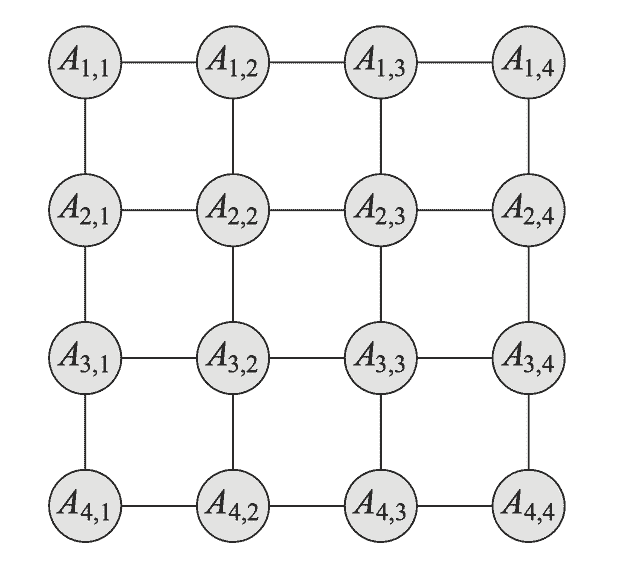
\includegraphics[width=0.3\textwidth]{Figs/a16.png}
    \caption{A pairwise Markov network (MRF) structured as a grid.}
    \label{fig:xfaserd}
\end{figure}
A subclass of Markov networks that arises in many contexts is that of pairwise Markov networks, representing distributions where all of the factors are over \tb{single variables or pairs of variables}. More precisely, a pairwise Markov network over a graph $\mathcal{H}$ is associated with:
\begin{enumerate}
    \item a set of \tb{node potentials} $\left\{\phi\left(X_{i}\right): i=1, \ldots, n\right\}$ and 
    \item a set of \tb{edge potentials} $\left\{\phi\left(X_{i}, X_{j}\right):\left(X_{i}, X_{j}\right) \in \mathcal{H}\right\}$
\end{enumerate}The overall distribution is (as always) the normalized product of all of the potentials (both node and edge).
\end{exma}
\begin{exma}\bfs{two different parameterization}\label{ex:idkkac}
Consider a fully connected graph.
If using maximal clique, the Markov network associated with this distribution is a \tb{single large clique} containing all variables. If we associate a factor with this single clique, it would be \tb{exponentially} large in the number of variables, whereas the original parameterization in terms of edges requires only a \tb{quadratic} number of parameters. 
\end{exma}
\subsubsection{Reduced Markov Networks}
If we have  $\boldsymbol{U}=\boldsymbol{u}$, it will only contribute to factors that are also consistent with this event.
More generally, we can define:

\begin{defa}\bfs{Factor Reduce}
 Let $\phi(\boldsymbol{Y})$ be a factor, and $\boldsymbol{U}=\boldsymbol{u}$ an assignment for $\boldsymbol{U} \subseteq \boldsymbol{Y}$. We define the reduction of the factor $\phi$ to the context $\boldsymbol{U}=\boldsymbol{u}$, denoted $\phi[\boldsymbol{U}=\boldsymbol{u}]$ (and abbreviated $\phi[\boldsymbol{u}]$ ), to be a factor over scope $\boldsymbol{Y}^{\prime}=\boldsymbol{Y}-\boldsymbol{U}$, such that
\begin{align*}
\phi[\boldsymbol{u}]\left(\boldsymbol{y}^{\prime}\right)=\phi\left(\boldsymbol{y}^{\prime}, \boldsymbol{u}\right)
\end{align*}
For $\boldsymbol{U} \not \subset \boldsymbol{Y}$, we define $\phi[\boldsymbol{u}]$ to be $\phi\left[\boldsymbol{U}^{\prime}=\boldsymbol{u}^{\prime}\right]$, where $\boldsymbol{U}^{\prime}=\boldsymbol{U} \cap \boldsymbol{Y}$, and $\boldsymbol{u}^{\prime}=\boldsymbol{u}\left\langle\boldsymbol{U}^{\prime}\right\rangle$, where $\boldsymbol{u}\left\langle\boldsymbol{U}^{\prime}\right\rangle$ denotes the assignment in $\boldsymbol{u}$ to the variables in $\boldsymbol{U}^{\prime}$.
\end{defa}
Now, consider a product of factors. An entry in the product is consistent with $\boldsymbol{u}$ if and only if it is a product of entries that are all consistent with $\boldsymbol{u}$. We can therefore define:
\begin{defa}\bfs{Reduced Gibbs Distribution}
 Let $P_{\Phi}$ be a Gibbs distribution parameterized by $\Phi=\left\{\phi_{1}, \ldots, \phi_{K}\right\}$ and let $\boldsymbol{u}$ be a context. The reduced Gibbs distribution $P_{\Phi}[\boldsymbol{u}]$ is the Gibbs distribution defined by the set of factors $\Phi[\boldsymbol{u}]=$ $\left\{\phi_{1}[\boldsymbol{u}], \ldots, \phi_{K}[\boldsymbol{u}]\right\}$

\end{defa}

Reducing the set of factors defining $P_{\Phi}$ to some context $\boldsymbol{u}$ corresponds directly to the operation of conditioning $P_{\Phi}$ on the observation $\boldsymbol{u}$. More formally:
\begin{lema}
Let $P_{\Phi}(\boldsymbol{X})$ be a Gibbs distribution. Then $P_{\Phi}[\boldsymbol{u}]=P_{\Phi}(\boldsymbol{W} \mid \boldsymbol{u})$ where $\boldsymbol{W}=\boldsymbol{X}-\boldsymbol{U}$.
\end{lema}
\begin{rema}\bfs{explanation}
This result immediately provides us with a construction for the Markov network that we obtain when we condition the associated distribution on some observation $\boldsymbol{u}$.
\end{rema}
\begin{defa}\bfs{Reduced Markov Network}
 Let $\mathcal{H}$ be a Markov network over $\boldsymbol{X}$ and $\boldsymbol{U}=\boldsymbol{u}$ a context. The reduced Markov network $\mathcal{H}[\boldsymbol{u}]$ is a Markov network over the nodes $\boldsymbol{W}=\boldsymbol{X}-\boldsymbol{U}$, where we have an edge $X-Y$ if there is an edge $X-Y$ in $\mathcal{H}$.
\end{defa}
\begin{lema}

Let $P_{\Phi}(\boldsymbol{X})$ be a Gibbs distribution that factorizes over $\mathcal{H}$, and $\boldsymbol{U}=\boldsymbol{u}$ a context. Then $P_{\Phi}[\boldsymbol{u}]$ factorizes over $\mathcal{H}[\boldsymbol{u}]$.
\end{lema}
\begin{rema}\bfs{explanation}
Note the contrast to the effect of conditioning in a Bayesian network: 
\begin{enumerate}
    \item Here, conditioning on a context $\boldsymbol{u}$ only eliminates edges from the graph; 
    \item In a Bayesian network, conditioning on evidence can activate a v-structure, creating new dependencies. 
\end{enumerate}
\end{rema}
\begin{exma}\bfs{Student Example} 
\begin{figure}[H]
    \centering
    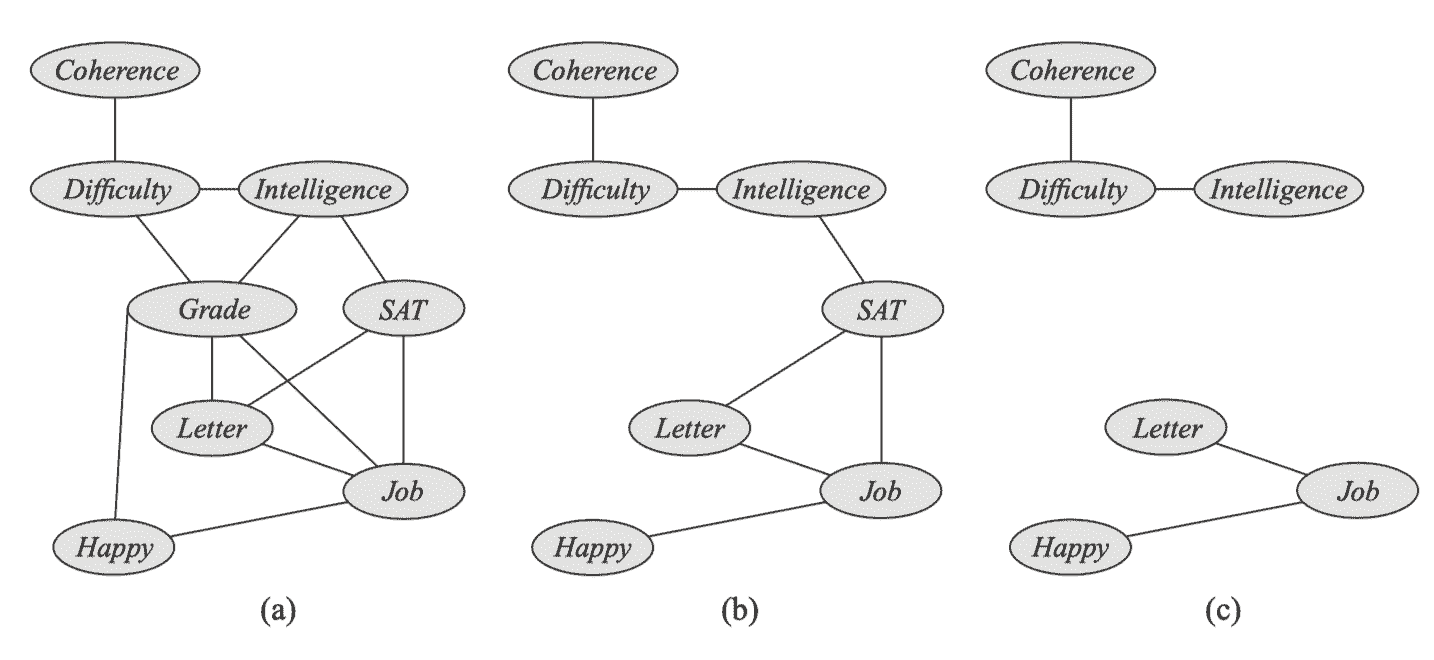
\includegraphics[width=0.9\textwidth]{Figs/a17.png}
    \caption{Markov networks for the factors in an extended Student example: (a) The initial set of factors; (b) Reduced to the context $G = g$; (c) Reduced to the context $G = g$, $S = s$.}
    \label{fig:qwevcc}
\end{figure}
We consider an extended Student Example as shown in the Markov network in \cref{fig:qwevcc}. (b) shows the same Markov network reduced over a context of the form $G=g$, and (c) shows the network reduced over a context of the form $G=g, S=s$. As we can see, the network structures are considerably simplified.
\end{exma}
\begin{exma}\bfs{Markov Networks for Computer Vision}\label{ex:mdfe}
Markov networks, typically called \tb{MRFs} in the vision community, have been used for a wide variety of visual processing tasks, such as image segmentation, removal of blur or noise, stereo reconstruction, object recognition, and many more.

In most of these applications, the network takes the structure of a \tb{pairwise MRF}, where the variables correspond to pixels and the edges (factors) to interactions between adjacent pixels in the grid that represents the image. The value space of the variables and the exact form of factors depend on the task. These models are usually formulated in terms of \tb{energies (negative log-potentials)}, so that values represent "penalties," and \tb{a lower value corresponds to a higher-probability configuration}.
\begin{enumerate}
    \item \tb{image denoising:}  Here, we have a \tb{node potential} for each pixel $X_{i}$ that penalizes large discrepancies from the observed pixel value $y_{i}$. The \tb{edge potential} encodes a preference for continuity between adjacent pixel values, penalizing cases where the inferred value for $X_{i}$ is too 
    far from the inferred pixel value for one of its neighbors $X_{j}$. However, it is important not to overpenalize true disparities (such as edges between objects or regions), leading to oversmoothing of the image. Thus, we bound the penalty, using, for example, \tb{some truncated norm}: $\epsilon\left(x_{i}, x_{j}\right)=\min (c\left\|x_{i}-x_{j}\right\|_{p}\mathrm{dist}_{\max }$ (for $p \in\{1,2\}$ ).
\item \tb{stereo reconstruction:}
The goal is to reconstruct the depth disparity of each pixel in the image. Here, the values of the variables represent some discretized version of the depth dimension (usually more finely discretized for distances close to the camera and more coarsely discretized as the distance from the camera increases). \tb{The individual node potential} for each pixel $X_{i}$ uses standard techniques from computer vision to estimate, from a pair of stereo images, the individual depth disparity of this pixel. \tb{The edge potentials}, precisely as before, often use a {truncated metric to enforce continuity of the depth estimates}, with the truncation avoiding an overpenalization of true depth disparities. Here, it is also quite common to make the penalty inversely proportional to the image gradient between the two pixels, allowing a smaller penalty to be applied in cases where a large image gradient suggests an edge between the pixels, possibly corresponding to an occlusion boundary.
\item \tb{image segmentation:}
The task is to partition the image pixels into regions corresponding to distinct parts of the scene. Each variable $X_{i}$ has a domain $\{1, \ldots, K\}$, where the value of $X_{i}$ represents a region assignment for pixel $i$ (for example, grass, water, sky, car). Since classifying every pixel can be computationally expensive, some state-of-the-art methods for image segmentation and other tasks first oversegment the image into superpixels (or small coherent regions) and classify each region - all pixels within a region are assigned the same label. The oversegmented image induces a graph in which there is one node for each superpixel and an edge between two nodes if the superpixels are adjacent (share a boundary) in the underlying image. We can now define our distribution in terms of this graph.
Features are extracted from the image for each pixel or superpixel. The appearance features depend on the specific task. In image segmentation, for example, features typically include statistics over color, texture, and location. Often the features are clustered or provided as input to local classifiers to reduce dimensionality. The features used in the model are then the soft cluster assignments or local classifier outputs for each superpixel. \tb{The node potential for a pixel or superpixel is then a function of these features}. We note that the factors used in defining this model depend on the specific values of the pixels in the image, so that each image defines a different probability distribution over the segment labels for the pixels or superpixels. In effect, the model used here is a \tb{conditional random field}, a concept that we define more formally in \cref{sec:crf}.

The model also contains an \tb{edge potential} between every pair of neighboring superpixels $X_{i}, X_{j}$. Most simply, this potential encodes a contiguity preference, with a penalty of $\lambda$ whenever $X_{i} \neq X_{j}$. Again, we can improve the model by making the penalty depend on the presence of an image gradient between the two pixels. An even better model does more than penalize discontinuities. We can have nondefault values for other class pairs, allowing us to encode the fact that we more often find tigers adjacent to vegetation than adjacent to water; we can even make the model depend on the relative pixel location, allowing us to encode the fact that we usually find water below vegetation, cars over roads, and sky above everything.
\end{enumerate}
\end{exma}

\subsection{Markov Network Independencies}\label{sec:ixsadf}
We give a formal presentation of the undirected graph as a representation of independence assertions, similar to what we have done in \cref{sec:ind_gra_bayes} for Bayesian network. 
\subsubsection{Basic Independencies: Separation}
As in the case of Bayesian networks, the graph structure in a Markov network can be viewed as encoding a set of independence assumptions. Intuitively, in Markov networks, probabilistic influence "flows" along the undirected paths in the graph, but it is blocked if we condition on the intervening nodes.
\begin{itemize}
    \item In \cref{sec:ind_gra_bayes}, for Bayesian network DAG, we define \tb{activeness} and \tb{d-seperation}, and then define the \tb{global Markov independencies set} $\calI(\calG)$. We show the \tb{soundness} (factorization $\Rightarrow$ $\mathcal{I}(\mathcal{G}) \subseteq \mathcal{I}(P)$) and \tb{completeness} of d-seperation.  
    \item In this section, for Markov network undirected graph, we define \tb{activeness} and \tb{seperation}, and then define the \tb{global Markov independencies set} $\calI(\calG)$. We show the \tb{soundness} (factorization $\Rightarrow$ $\mathcal{I}(\mathcal{G}) \subseteq \mathcal{I}(P)$) and \tb{completeness} of seperation. 
\end{itemize}
\begin{defa}\bfs{Path Activeness}
Let $\mathcal{H}$ be a Markov network structure, and let $X_{1}-\ldots-X_{k}$ be a path (trail) in $\mathcal{H} .$ Let $\boldsymbol{Z} \subseteq \mathcal{X}$ be a set of observed variables. The path $X_{1}-\ldots-X_{k}$ is \tb{active} given $\boldsymbol{Z}$ if none of the $X_{i}$'s, $i=1, \ldots, k$, is in $\boldsymbol{Z}$.
\end{defa}
\begin{defa}\bfs{Separation}
We say that a set of nodes $\boldsymbol{Z}$ separates $\boldsymbol{X}$ and $\boldsymbol{Y}$ in $\mathcal{H}$, denoted $\operatorname{sep}_{\mathcal{H}}(\boldsymbol{X} ; \boldsymbol{Y} \mid \boldsymbol{Z})$, if there is \tb{no active path between any node} $X \in X$ and $Y \in Y$ given $Z$. We define the \tb{global independencies} associated with $\mathcal{H}$ to be:
\begin{align*}
\mathcal{I}(\mathcal{H})=\left\{(\boldsymbol{X} \perp \boldsymbol{Y} \mid \boldsymbol{Z}): \mathrm{sep}_{\mathcal{H}}(\boldsymbol{X} ; \boldsymbol{Y} \mid \boldsymbol{Z})\right\}
\end{align*}
\end{defa}
\begin{rema}\bfs{reminder}
Our definition of \tb{separation} has been based on our intuitions regarding flow of influence (activeness). In \cref{thm:sep1} we give proofs that \tb{d-separation} indeed corresponds to independencies for Gibbs distribution defined over the graph, so here $\mathcal{I}(\mathcal{G})$ is indeed set of independencies. In other words, the separation criterion is \tb{sound} for detecting independence properties in distributions over $\mathcal{H}$.
\end{rema}

\begin{rema}\bfs{monotonic and limitation}
If $\operatorname{sep}_{\mathcal{H}}(\boldsymbol{X} ; \boldsymbol{Y} \mid \boldsymbol{Z})$, then $\operatorname{sep}_{\mathcal{H}}\left(\boldsymbol{X} ; \boldsymbol{Y} \mid \boldsymbol{Z}^{\prime}\right)$ for any $\boldsymbol{Z}^{\prime} \supset \boldsymbol{Z}$.  It implies the limitation of Markov network graph: the {$v$-structure} cannot be expressed using a Markov network since  given the middle node, the other two are dependent, while given the empty set, the two nodes are independent.
\end{rema}
\paragraph{Soundness of Separation and Hammersley-Clifford Theorem}\label{sec:mdrfefa}
We now assert the equivalence between the \tb{Markov factorization} of a distribution $P$ over a graph $\mathcal{H}$ and the assertion that $\mathcal{H}$ is an \tb{I-map} (see \cref{def:Imapglobal}) for $P$: $\mathcal{I}(\mathcal{H}) \subseteq \mathcal{I}(P)$.
\begin{rema}
Recall that Markov factorization \cref{def:Markov_fac} is Gibbs distribution with constraints that factors only are over cliques.
\end{rema}

$\bullet$ \tb{Factorization to I-map:}
\begin{thma}\bfs{D-separation and Independence I}\label{thm:sep1}
Let $P$ be a distribution over $\mathcal{X}$, and $\mathcal{H}$ a Markov network structure over $\mathcal{X}$. If $P$ is a Gibbs distribution that factorizes over $\mathcal{H}$, then $\mathcal{H}$ is an I-map for $P$: $\mathcal{I}(\mathcal{H}) \subseteq \mathcal{I}(P)$
\end{thma}
\begin{rema}
This is the analogue to \cref{thm:dsep1}. Here it asserts that a Gibbs distribution  satisfies the independencies associated with the graph. In other words, this result states the \tb{soundness} of the separation.
\end{rema}
\begin{lema}\label{lem:okkse}
Let $\boldsymbol{X}, \boldsymbol{Y}, \boldsymbol{Z}$ be three disjoint subsets of variables such that $\mathcal{X}=\boldsymbol{X} \cup \boldsymbol{Y} \cup \boldsymbol{Z}$. Prove that $P \models(\boldsymbol{X} \perp$ $\boldsymbol{Y} \mid \boldsymbol{Z}$ ) if and only if we can write $P$ in the form:
\begin{align*}
P(\mathcal{X})=\phi_{1}(\boldsymbol{X}, \boldsymbol{Z}) \phi_{2}(\boldsymbol{Y}, \boldsymbol{Z}) .
\end{align*}
\end{lema}
\begin{proof} (of \cref{lem:okkse})
 Easy from definition. Just omit.
\end{proof}
\begin{proof} (of \cref{thm:sep1})
 Let $\boldsymbol{X}, \boldsymbol{Y}, \boldsymbol{Z}$ be any three disjoint subsets in $\mathcal{X}$ such that $\boldsymbol{Z}$ separates $\boldsymbol{X}$ and $\boldsymbol{Y}$ in $\mathcal{H}$. We want to show that $P \models(\boldsymbol{X} \perp \boldsymbol{Y} \mid \boldsymbol{Z})$.

We start by considering the case where $\boldsymbol{X} \cup \boldsymbol{Y} \cup \boldsymbol{Z}=\mathcal{X}$. As $\boldsymbol{Z}$ separates $\boldsymbol{X}$ from $\boldsymbol{Y}$, there are no direct edges between $\boldsymbol{X}$ and $\boldsymbol{Y}$. Hence, \tb{any clique in $\mathcal{H}$ is fully contained either in $\boldsymbol{X} \cup \boldsymbol{Z}$ or in $\boldsymbol{Y} \cup \boldsymbol{Z}$}. Let $\mathcal{I}_{\boldsymbol{X}}$ be the indexes of the set of cliques that are contained in $\boldsymbol{X} \cup \boldsymbol{Z}$, and let $\mathcal{I}_{Y}$ be the indexes of the remaining cliques. We know that
\begin{align*}
P\left(X_{1}, \ldots, X_{n}\right)=\frac{1}{Z} \prod_{i \in \mathcal{I}_{\boldsymbol{X}}} \phi_{i}\left(\boldsymbol{D}_{i}\right) \cdot \prod_{i \in \mathcal{I}_{\boldsymbol{Y}}} \phi_{i}\left(\boldsymbol{D}_{i}\right)
\end{align*}
As we discussed, none of the factors in the first product involve any variable in $\boldsymbol{Y}$, and none in the second product involve any variable in $\boldsymbol{X}$. Hence, we can rewrite this product in the form:
\begin{align*}
P\left(X_{1}, \ldots, X_{n}\right)=\frac{1}{Z} f(\boldsymbol{X}, \boldsymbol{Z}) g(\boldsymbol{Y}, \boldsymbol{Z})
\end{align*}
From this decomposition, the desired independence follows \cref{lem:okkse}.
Now consider the case where $\boldsymbol{X} \cup \boldsymbol{Y} \cup \boldsymbol{Z} \subset \mathcal{X}$. Let $\boldsymbol{U}=\mathcal{X}-(\boldsymbol{X} \cup \boldsymbol{Y} \cup \boldsymbol{Z})$. We can partition $\boldsymbol{U}$ into two disjoint sets $\boldsymbol{U}_{1}$ and $\boldsymbol{U}_{2}$ such that $\boldsymbol{Z}$ separates $\boldsymbol{X} \cup \boldsymbol{U}_{1}$ from $\boldsymbol{Y} \cup \boldsymbol{U}_{2}$ in $\mathcal{H}$. Using the preceding argument, we conclude that $P \models\left(\boldsymbol{X}, \boldsymbol{U}_{1} \perp \boldsymbol{Y}, \boldsymbol{U}_{2} \mid \boldsymbol{Z}\right)$. Using the decomposition property (see Corollary 2.17 in "Basic Graphical Models Notes"), we conclude that $P \models(\boldsymbol{X} \perp \boldsymbol{Y} \mid \boldsymbol{Z})$.
\end{proof}

$\bullet$ \tb{I-Map to Factorization:}

We next state Hammersley-Clifford Theorem which is the analogue to \cref{thm:imap2frac}.
\begin{thma}\bfs{Hammersley-Clifford Theorem}\label{thm:Hammersley}
Let $P$ be a positive distribution over $\mathcal{X}$, and $\mathcal{H}$ a Markov network graph over $\mathcal{X}$. If $\mathcal{H}$ is an I-map for $P$, then $P$ is a Gibbs distribution that factorizes over $\mathcal{H}$.
\end{thma}
\begin{rema}
As we will show, it holds only under the additional assumption that $P$ is a positive distribution.
\end{rema}
\begin{proof}
 See the proof in "Basic Graphical Models Notes".
\end{proof}

\begin{rema}
 So we have that:
 
 \centerline{\tb{``positive distribution $P$ factorizes over a Markov network $\mathcal{H}$'' $\Longleftrightarrow \mathcal{H}$ is an I-map of $P$.}}
\end{rema} 

\paragraph{Completeness of Separation}
\tb{Question:} separation detects all possible independencies (strong completeness)? i.e. if $P$ factorizes according to $\mathcal{H}$, do we have $\mathcal{I}(P) \subseteq \mathcal{I}(\calG)$?

\tb{Answer:} No.

\tb{Weak Completeness:} If $(X \perp Y \mid \boldsymbol{Z})$ in \tb{all distributions $P$ that factorize over $\mathcal{H}$}, then {$\mathrm{sep}$}$_{\mathcal{H}}(X ; Y \mid \boldsymbol{Z}) .$  In other words:
\begin{thma}\bfs{D-separation and Independence II}\label{thm:sep2}\\
\centerline{We have $\cap_{P\in S}\mathcal{I}(P) \subseteq \mathcal{I}(\calH)$, where  $S\coloneqq \{P: P \text{ factorizes w.r.t. $\mathcal{H}$}\}$.}
\end{thma}
\begin{proof} We prove the equivalent contrapositive statement :

``Let $\mathcal{H}$ be a Markov network structure. If $X$ and $Y$ are not separated given $\boldsymbol{Z}$ in $\mathcal{H}$, then $X$ and $Y$ are dependent given $Z$ in some distribution $P$ that factorizes over $\mathcal{H}$.''

The proof is a constructive one: we construct a distribution $P$ that factorizes over $\mathcal{H}$ where $X$ and $Y$ are dependent. We assume, without loss of generality, that all variables are binary-valued. If this is not the case, we can treat them as binary-valued by restricting attention to two distinguished values for each variable.

By assumption, $X$ and $Y$ are not separated given $\boldsymbol{Z}$ in $\mathcal{H}$; hence, they must be connected by some unblocked trail. Let $X=U_{1}-U_{2}-\ldots-U_{k}=Y$ be some minimal trail in the graph such that, for all $i, U_{i} \notin Z$, where we define a minimal trail in $\mathcal{H}$ to be a path with no shortcuts: thus, for any $i$ and $j \neq i \pm 1$, there is no edge $U_{i}-U_{j} .$ We can always find such a path: If we have a nonminimal path where we have $U_{i}-U_{j}$ for $j>i+1$, we can always "shortcut" the original trail, converting it to one that goes directly from $U_{i}$ to $U_{j}$.

For any $i=1, \ldots, k-1$, since there is an edge $U_{i}-U_{i+1}$, it follows that $U_{i}, U_{i+1}$ must both appear in some clique $\boldsymbol{C}_{i} .$ Choose constant $W$. For each $i$ we define the clique potential $\phi_{i}\left(\boldsymbol{C}_{i}\right)=W$ if $U_{i}=U_{i+1}$ and weight $1$ otherwise, regardless of the values of the other variables in the clique. Note that the cliques $\boldsymbol{C}_{i}$ for $U_{i}, U_{i+1}$ and $\boldsymbol{C}_{j}$ for $U_{j}, U_{j+1}$ must be different cliques: If $\boldsymbol{C}_{i}=\boldsymbol{C}_{j}$, then $U_{j}$ is in the same clique as $U_{i}$, and we have an edge $U_{i}-U_{j}$, contradicting the minimality of the trail. Hence, we can define the clique potential for each clique $\boldsymbol{C}_{i}$ separately. We define the clique potential for any other clique to be uniformly $1$.

We now consider the distribution $P$ resulting from multiplying all of these clique potentials. Intuitively, the distribution $P\left(U_{1}, \ldots, U_{k}\right)$ is simply the distribution defined by multiplying the pairwise factors for the pairs $U_{i}, U_{i+1}$, regardless of the other variables (including the ones in $\boldsymbol{Z}$ ). One can verify that, in $P\left(U_{1}, \ldots, U_{k}\right)$, we have that $X=U_{1}$ and $Y=U_{k}$ are dependent.  As ${W} \rightarrow \infty$, we have $P(X=Y)=1$ while $P(X)$ could be set as $1/|\mathrm{Val}(X)|$.
\end{proof}


We can use the same argument as \cref{thm:dsep3} to conclude that: 
\begin{thma}\bfs{D-separation and Independence III}\label{thm:sep3} \\
For \tb{almost all} distributions $P$ that factorize over $\mathcal{H}$, that is, for all distributions except for a set of measure zero in the space of factor parameterizations, we have that $\mathcal{I}(P)=\mathcal{I}(\mathcal{H})$.
\end{thma}


Once again, we can view this result as telling us that our definition of $\mathcal{I}(\mathcal{H})$ is the maximal one. For any independence assertion that is not a consequence of separation in $\mathcal{H}$, we can always find a counterexample distribution $P$ that factorizes over $\mathcal{H}$.

\subsubsection{Independencies: Local, Global and Pairwise}\label{sec:loc_pair_glo}
In a Bayesian network, we provided two definitions: the local independencies $\calI_\ell(\calG)$ (each node is independent of its nondescendants given its parents), and the global independencies  $\calI(\calG)$ induced by d-separation. As we have showed, ``same $\calI_\ell(\calG)$'' $\Leftrightarrow$ ``same $\calI(\calG)$''.

We have define the global independencies for Markov networks. We next provide two local independencies for Markov networks, and show the equivalence between them under positive distribution assumption.

\begin{defa}\bfs{Pairwise Independence}
Let $\mathcal{H}$ be a Markov network. We define the \tb{pairwise independencies} associated with $\mathcal{H}$ to be:
\begin{align*}
\mathcal{I}_{p}(\mathcal{H})=\{(X \perp Y \mid \mathcal{X}-\{X, Y\}): X-Y \notin \mathcal{H}\} .
\end{align*}
\end{defa}
\begin{rema}\bfs{explanation}
\begin{enumerate}
    \item  Similar to the Bayesian network, whenever two variables are directly connected, they have the potential of being directly correlated in a way that is not mediated by other variables. 
    \item Conversely, when two variables are not directly linked, there must be some way of rendering them conditionally independent. Specifically, we can require that $X$ and $Y$ be independent given \tb{all other nodes} in the graph.
\end{enumerate}
\end{rema}


The second local definition is an undirected analogue to the local independencies associated with a Bayesian network. It is based on the intuition that we can block all influences on a node by conditioning on its immediate neighbors.
\begin{defa}\bfs{Local Independence}
For a given graph $\mathcal{H}$, we define  $\mathrm{Nb}_{\mathcal{H}}(X)$ to be the \tb{neighbors} of $X$ in $\mathcal{H}$. We define the \tb{local independencies} associated with $\mathcal{H}$ to be:
\begin{align*}
\mathcal{I}_{\ell}(\mathcal{H})=\left\{\left(X \perp \mathcal{X}-\{X\}-\mathrm{Nb}_{\calH}(X) \mid \mathrm{Nb}_{\calH}(X)\right): X \in \mathcal{X}\right\} .
\end{align*}
\end{defa}
\begin{rema}\bfs{explanation}
In other words, the local independencies state that $X$ is independent of the rest of the nodes in the graph given its immediate neighbors. In \cite{koller2009probabilistic} it uses $\mathrm{MB}_{\mathcal{H}}(X)$ which is defined twice. We abandon this.
\end{rema}
\begin{thma}
The following three statements are equivalent for a \tb{positive distribution $P$}:
\begin{enumerate}
    \item  $P \models \mathcal{I}_{\ell}(\mathcal{H})$.
    \item $P \models \mathcal{I}_{p}(\mathcal{H})$.
    \item $P \models \mathcal{I}(\mathcal{H})$.
\end{enumerate}
\end{thma}
This equivalence relies on the positivity assumption. In particular, for nonpositive distributions, we can provide examples of a distribution $P$ that satisfies one of these properties, but not the stronger one.
\begin{exma}
Let $P$ be any distribution over $\mathcal{X}=\left\{X_{1}, \ldots, X_{n}\right\} ;$ let $\mathcal{X}^{\prime}=\left\{X_{1}^{\prime}, \ldots, X_{n}^{\prime}\right\} .$ We now construct a distribution $P^{\prime}\left(\mathcal{X}, \mathcal{X}^{\prime}\right)$ whose marginal over $X_{1}, \ldots, X_{n}$ is the same as $P$, and where $X_{i}^{\prime}$ is deterministically equal to $X_{i}$. Let $\mathcal{H}$ be a Markov network over $\mathcal{X}, \mathcal{X}^{\prime}$ that contains no edges other than $X_{i}-X_{i}^{\prime}$. Then, in $P^{\prime}, X_{i}$ is independent of the rest of the variables in the network given its neighbor $X_{i}^{\prime}$, and similarly for $X_{i}^{\prime}$; thus, $\mathcal{H}$ satisfies the local independencies for every node in the network. Yet clearly $\mathcal{H}$ is not an I-map for $P^{\prime}$, since $\mathcal{H}$ makes many independence assertions regarding the $X_{i}$'s that do not hold in $P$ (or in $P^{\prime}$ ).
\end{exma}


\subsubsection{From Distributions to Graphs: Minimal I-Maps}\label{sec:dis2imapmark}
The \tb{{minimal I-map}} defined in \cref{def:nmfae} still holds here. And the complete undirected graph is still an I-map for any Gibbs distribution, yet it does not reveal any of the independence structure in the distribution. We recall the definition here: \emph{A graph $\mathcal{K}$ is a minimal I-map for a set of independencies $\mathcal{I}$ if it is an I-map for $\mathcal{I}$, and if the \tb{removal of even a single edge} from $\mathcal{K}$ renders it not an I-map.}

$\bullet$ \tb{Two Possible Approaches to Construct Minimal I-map:} 

We can use the local and pairwise Markov independencies introduced in \cref{sec:loc_pair_glo} to do the construction:
\begin{enumerate}
    \item \tb{pairwise independence based:}  If the edge $\{X, Y\}$ is not in $\mathcal{H}$, then $X$ and $Y$ must be independent given all other nodes in the graph, regardless of which other edges the graph contains:
    \begin{enumerate}
        \item Find all pairs of nodes $X$ and $Y$ such that
\begin{align}
P \not \models(X \perp Y \mid \mathcal{X}-\{X, Y\})\label{eq:oiefcz}
\end{align}
\item Define $\mathcal{H}$ to include an edge $X-Y$ for all the found pairs.
    \end{enumerate}
    \item \tb{local independence based:}  We first define:
    \begin{defa}\bfs{Markov Blanket over Distribution}\label{eq:nefa}
    A set $\boldsymbol{U}$ is a \tb{Markov blanket} of $X$ in a distribution $P$ if $X \notin \boldsymbol{U}$ and if $\boldsymbol{U}$ is a minimal set of nodes such that
\begin{align}
(X \perp \mathcal{X}-\{X\}-\boldsymbol{U} \mid \boldsymbol{U}) \in \mathcal{I}(P)\label{eq:iierfz}
\end{align}
    \end{defa}
    We then conduct:
    \begin{enumerate}
    \item Find $\mathrm{MB}_{P}(X)$ for each $X$.
        \item Define a graph $\mathcal{H}$ by introducing an edge $\{X, Y\}$ for all $X$ and all $Y \in \mathrm{MB}_{P}(X)$.
    \end{enumerate}
\end{enumerate}
We also give a definition of Markov blanket over graph which will be used later, e.g. \cref{sec:meqkdka}.
\begin{defa}\bfs{Markov Blanket over Graph}\label{eq:zcdad}
    A set $\boldsymbol{U}$ is a \tb{Markov blanket} of $X$ in a (any type) graph if $X \notin \boldsymbol{U}$ and if $\boldsymbol{U}$ is a minimal set of nodes such that
\begin{align}
(X \perp \mathcal{X}-\{X\}-\boldsymbol{U} \mid \boldsymbol{U}) \in \mathcal{I}(P)\label{eq:zvdaff}
\end{align}
for all distribution factorizable over graph.
    \end{defa}

\tb{Question:} can we get unique I-map now?

\tb{Answer:} Yes. Any positive distribution $P$ has a unique minimal I-map, both the two approaches get the same map.
\begin{thma}
Let $P$ be a positive distribution, we conclude that the minimal I-map for $P$ is \tb{unique}. Let $\mathcal{H}$ be defined by introducing an edge $\{X, Y\}$ for all $X, Y$ for which equation \cref{eq:oiefcz} holds. Then the Markov network $\mathcal{H}$ is the \tb{unique} minimal I-map for $P$.
\end{thma}
\begin{proof}
The fact that $\mathcal{H}$ is an I-map for $P$ follows immediately from fact that $P$, by construction, satisfies $\mathcal{I}_{p}(\mathcal{H})$, and, therefore, also satisfies $\mathcal{I}(\mathcal{H})$. The fact that it is minimal follows from the fact that if we eliminate some edge $\{X, Y\}$ from $\mathcal{H}$, the new graph would imply the pairwise independence $(X \perp Y \mid \mathcal{X}-\{X, Y\})$, which we know to be false for $P$ (otherwise, the edge would have been omitted in the construction of $\mathcal{H}$ ). The uniqueness of the minimal I-map also follows trivially: By the same argument, any other I-map $\mathcal{H}^{\prime}$ for $P$ must contain at least the edges in $\mathcal{H}$ and is therefore either equal to $\mathcal{H}$ or contains additional edges and is therefore not minimal.
\end{proof} 
It remains to show that the second definition results in the same minimal I-map.
\begin{thma}
Let $P$ be a positive distribution. For each node $X$, let $\mathrm{MB}_{P}(X)$ be a minimal set of nodes $\boldsymbol{U}$ satisfying equation \cref{eq:iierfz}. We define a graph $\mathcal{H}$ by introducing an edge $\{X, Y\}$ for all $X$ and all $Y \in \mathrm{MB}_{P}(X)$. Then the Markov network $\mathcal{H}$ is the unique minimal I-map for $P$.
\end{thma}

For nonpositive distributions, we however cannot use the above two approaches to construct I-map. For example, deterministic relations between variables can lead to failure in the construction based on local and pairwise independence.
\begin{exma}
Suppose that $A$ and $B$ are two variables that are identical to each other and that both $C$ and $D$ are variables that correlated to both $A$ and $B$ so that $(C \perp D \mid A, B)$ holds. Since $A$ is identical to $B$, we have that both $(A, D \perp C \mid B)$ and $(B, D \perp C \mid A)$ hold. In other words, it suffices to observe one of these two variables to capture the relevant information both have about $C$ and separate $C$ from $D$. In this case the Markov blanket of $C$ is not uniquely defined. This ambiguity leads to the failure of both local and pairwise constructions. Clearly, identical variables are only one way of getting such ambiguities in local independencies. Once we allow nonpositive distribution, other distributions can have similar problems.
\end{exma}

\tb{Question:} Can we get perfect map?

\tb{Answer:} No. Perfect map is not guaranteed for every distribution even for positive distributions.

\subsection{Parameterization Revisited: Generalization and Overparameterization}
\subsubsection{Finer-Grained Parameterization}
Factor graphs will make the factor parameterization more clear. Log-Linear models is one kind of re-parameter, a generalization of the original Markov factor parameterization. A little bit similar to the reparametrization of canonical exponential families in ``Mathematical Statistics Notes''.
\paragraph{Factor Graphs}

A Markov network structure does not generally reveal all of the structure in a Gibbs parameterization. In particular, one cannot tell from the graph structure whether the factors of any distribution that factorizable over the graph involve maximal cliques or subsets thereof. The example of fully connected graph shown in \cref{ex:idkkac} using pairs or the single clique is an illustration for this.

An alternative representation that makes this structure explicit is a \tb{factor graph}. 

\begin{defa}\bfs{Factor Graphs, Factorization}
A \tb{factor graph} $\mathcal{F}$ is an undirected graph containing two types of nodes: \tb{variable nodes} (denoted as ovals) and \tb{factor nodes} (denoted as squares). The graph only contains edges between variable nodes and factor nodes. A factor graph $\mathcal{F}$ is \tb{parameterized} by a set of factors, where each factor node $V_{\phi}$ is associated with precisely one factor $\phi$, whose \tb{scope} is the set of variables that are \tb{neighbors} of $V_{\phi}$ in the graph.

A distribution $P$ \tb{factorizes} over $\mathcal{F}$ if it can be represented as a set of factors of this form.
\end{defa}
\begin{exma}
See \cref{fig:kldda}. Although the Markov networks for these two distributions are identical, their factor graphs make explicit the difference in their factorization.
\end{exma}
\begin{figure}[H]
    \centering
    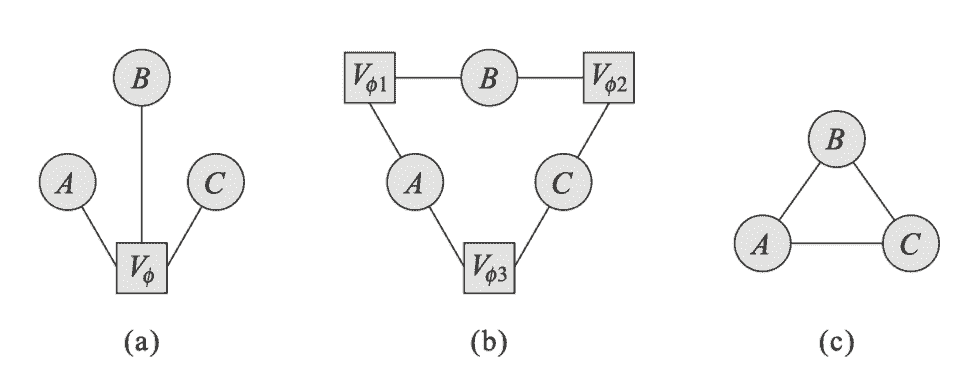
\includegraphics[width=0.7\textwidth]{Figs/a18.png}
    \caption{Different factor graphs for the same Markov network: (a) One factor graph over $A$, $B$, $C$, with a single factor over all three variables. (b) An alternative factor graph, with three pairwise factors. (c) The induced Markov network for both is a clique over $A$, $B$, $C$.}
    \label{fig:kldda}
\end{figure}
\paragraph{Log-Linear Models}\label{sec:loglinearmodel}
Log-linear models are the re-parameter using \tb{sum of factors} and is a generalization of the original Markov factor parameterization which uses \tb{product of clique factors}. We first introduce a \tb{special log-linear} model which is equivalent to Markov factorization\cref{eq:cli_fac}.

$\bullet$  \tb{energy function:}

\begin{defa}\bfs{Energy Function}
We can rewrite a factor $\phi(\boldsymbol{D})$ as
\begin{align*}
\phi(\boldsymbol{D})=\exp (-\epsilon(\boldsymbol{D}))
\end{align*}
where the \tb{energy function} $\epsilon(\boldsymbol{D})$ is: $$\epsilon(\boldsymbol{D})=-\ln \phi(\boldsymbol{D}).$$
\end{defa}
 \begin{rema}
 Remember that ``large energy, low probability''
 \end{rema}
  In this logarithmic representation, we have
\begin{align*}
P\left(X_{1}, \ldots, X_{n}\right) \propto \exp \left[-\sum_{i=1}^{m} \epsilon_{i}\left(\boldsymbol{D}_{i}\right)\right]
\end{align*}

$\bullet$  \tb{General Framework :}

% Note previously we does not talk about the feature of note.
We can provide a general framework for capturing such structure using the following notion:
\begin{defa}\bfs{Feature}
Let $\boldsymbol{D}$ be a subset of variables. We define a \tb{feature} $f(\boldsymbol{D})$ to be a function from $\mathrm{Val}(\boldsymbol{D})$ to $\mathbb{R}$.
\end{defa}
\begin{rema}
Just take it as a rename of factor function under the log-linear models. One type of feature of particular interest is the indicator feature that takes on value $1$ for some values $\boldsymbol{y} \in \mathrm{Val}(\boldsymbol{D})$ and $0$ otherwise.
\end{rema}

 \begin{defa}\bfs{Log-Linear Model}\label{def:loglinear}
 A distribution $P$ is a \tb{log-linear} model over a Markov network $\mathcal{H}$ if it is associated with:
 \begin{itemize}
     \item \tb{a set of features} $\mathcal{F}=\left\{f_{1}\left(\boldsymbol{D}_{1}\right), \ldots, f_{k}\left(\boldsymbol{D}_{k}\right)\right\}$, where each $\boldsymbol{D}_{i}$ is a complete subgraph in $\mathcal{H}$,
     \item \tb{a set of weights} $w_{1}, \ldots, w_{k}$,
such that
\begin{align*}
P\left(X_{1}, \ldots, X_{n}\right)=\frac{1}{Z} \exp \left[-\sum_{i=1}^{k} w_{i} f_{i}\left(\boldsymbol{D}_{i}\right)\right]
\end{align*}
 \end{itemize}
 \end{defa}
\begin{rema}
Set $w=1$, we get the  energy function as a special case.
\end{rema}
\begin{exma}\bfs{Ising Models and Boltzmann Machines}
One of the earliest types of Markov network models is the Ising model, which first arose in statistical physics as a model for the energy of a physical system involving a system of interacting atoms. In these systems, each atom is associated with a binary-valued random variable $X_{i} \in\{+1,-1\}$, whose value defines the direction of the atom's spin. \tb{The energy function associated with the edges is defined by a particularly simple parametric form:}
\begin{align}
\epsilon_{i, j}\left(x_{i}, x_{j}\right)=w_{i, j} x_{i} x_{j}\label{eq:ujxjdda}
\end{align}
This energy is symmetric in $X_{i}, X_{j}$; it makes a contribution of $w_{i, j}$ to the energy function when $X_{i}=X_{j}$ (so both atoms have the same spin) and a contribution of $-w_{i, j}$ otherwise. Our model also contains a set of parameters $u_{i}$ that encode individual node potentials; these bias individual variables to have one spin or another.
As usual, the energy function defines the following distribution:
\begin{align*}
P(\xi)=\frac{1}{Z} \exp \left(-\sum_{i<j} w_{i, j} x_{i} x_{j}-\sum_{i} u_{i} x_{i}\right)
\end{align*}
As we can see, when $w_{i, j}>0$ the model prefers to align the spins of the two atoms; in this case, the interaction is called ferromagnetic. When $w_{i, j}<0$ the interaction is called antiferromagnetic. When $w_{i, j}=0$ the atoms are non-interacting.


Related to the Ising model is the \tb{Boltzmann distribution}; here, the variables are usually taken to have values $\{0,1\}$, but still with the energy form of equation \cref{eq:ujxjdda}. Here, we get a nonzero contribution to the model from an edge $\left(X_{i}, X_{j}\right)$ only when $X_{i}=X_{j}=1$; however, the resulting energy can still be reformulated in terms of an Ising model 

The popularity of the Boltzmann machine was primarily driven by its similarity to an activation model for neurons. To understand the relationship, we note that the probability distribution over each variable $X_{i}$ given an assignment to is neighbors is $\operatorname{sigmoid}(z)$ where
\begin{align*}
z=-\left(\sum_j w_{i, j} x_{j}\right)-w_{i} .
\end{align*}
This function is a sigmoid of a weighted combination of $X_{i}$'s neighbors, weighted by the strength and direction of the connections between them. This is the simplest but also most popular mathematical approximation of the function employed by a neuron in the brain. Thus, if we imagine a process by which the network continuously adapts its assignment by resampling the value of each variable as a stochastic function of its neighbors, then the "activation" probability of each variable resembles a neuron's activity. This model is a very simple variant of a stochastic, recurrent neural network.
\end{exma}

\begin{exma}\bfs{Metric MRFs}
One important class of MRFs comprises those used for labeling. Here, we have a graph of nodes $X_{1}, \ldots, X_{n}$ related by a set of edges $\mathcal{E}$, and we wish to assign to each $X_{i}$ a label in the space $\mathcal{V}=\left\{v_{1}, \ldots, v_{K}\right\} .$ Each node, taken in isolation, has its preferences among the possible labels. However, we also want to impose a \tb{soft "smoothness" constraint} over the graph, in that neighboring nodes should take "similar" values.

We encode the \tb{individual node preferences as node potentials in a pairwise MRF and the smoothness preferences as edge potentials}. For reasons that will become clear, it is traditional to encode these models in negative log-space, using \tb{energy functions}. As our objective in these models is inevitably the \tb{MAP objective}, we can also ignore the partition function, and simply consider the energy function:
\begin{align*}
E\left(x_{1}, \ldots, x_{n}\right)=\sum_{i} \epsilon_{i}\left(x_{i}\right)+\sum_{(i, j) \in \mathcal{E}} \epsilon_{i, j}\left(x_{i}, x_{j}\right)
\end{align*}
Our goal is then to minimize the energy:
\begin{align*}
\arg \min _{x_{1}, \ldots, x_{n}} E\left(x_{1}, \ldots, x_{n}\right)
\end{align*}
We now need to provide a formal definition for the intuition of "smoothness" described earlier. There are many different types of conditions that we can impose; different conditions allow different methods to be applied.

One of the simplest in this class of models is a slight variant of the Ising model, where we have that, for any $i, j:$
\begin{align*}
\epsilon_{i, j}\left(x_{i}, x_{j}\right)= \begin{cases}0 & x_{i}=x_{j} \\ \lambda_{i, j} & x_{i} \neq x_{j}\end{cases}
\end{align*}
for $\lambda_{i, j} \geq 0$. An even broader class contains models where we have a \tb{distance function on the labels}, and where we prefer neighboring nodes to have labels that are a smaller distance apart.
\end{exma} 
\subsubsection{Overparameterization}
Intuitively, the standard Markov network representation gives us too many places to account for the influence of variables in shared cliques. Thus, the same distribution can be represented as a Markov network (of a given structure) in infinitely many ways. 
\begin{exma}\bfs{Markov network parameterization is generally overparameterized}
\begin{enumerate}
    \item Most obviously, if our graph is a single clique over $n$ binary variables $X_{1}, \ldots, X_{n}$, then the network is associated with a clique potential that has $2^{n}$ parameters, whereas the joint distribution only has $2^{n}-1$ independent parameters.
    \item Consider a pair of cliques $\{A, B\}$ and $\{B, C\}$. The energy function $\epsilon_{1}(A, B)$ (or its corresponding clique potential) contains information not only about the interaction between $A$ and $B$, but also about the distribution of the individual variables $A$ and $B$. Similarly, $\epsilon_{2}(B, C)$ gives us information about the individual variables $B$ and $C$. The information about $B$ can be placed in either of the two cliques, or its contribution can be split between them in arbitrary ways, resulting in many different ways of specifying the same distribution.
\end{enumerate}
\end{exma}

\paragraph{Canonical Parameterization}
The canonical parameterization provides one very natural approach to avoiding the ambiguity in the parameterization of a Gibbs distribution $P$. The canonical parameterization requires that the distribution $P$ \tb{be positive}. 

It is most convenient to describe this parameterization using \tb{energy functions} rather then clique potentials. For this reason, we consider a \tb{logtransform of $P$}. For any assignment $\xi$ to $\mathcal{X}$, we use $\ell(\xi)$ to denote $\ln P(\xi)$. 


$\bullet$ \tb{Some concepts:}

\begin{itemize}
    \item The canonical parameterization is defined relative to a \tb{particular fixed assignment} $\xi^{*}=$ $\left(x_{1}^{*}, \ldots, x_{n}^{*}\right)$ to the network variables $\mathcal{X}$. This assignment can be chosen arbitrarily. In "Basic Graphical Models Notes", we choose an arbitrary assignment, denoted as $0$ for each node and call it "black".
    \item For any subset of variables $\boldsymbol{Z}$, and any assignment $\boldsymbol{x}$ to some subset of $\mathcal{X}$ that contains $\boldsymbol{Z}$, we define the \tb{assignment} $\boldsymbol{x}_{\boldsymbol{Z}}$ to be $\boldsymbol{x}\langle\boldsymbol{Z}\rangle$, that is, the assignment in $\boldsymbol{x}$ to the variables in $\boldsymbol{Z}$. 
    \item We define \tb{assignment $\xi_{-Z}^{*}$} to be $\xi^{*}\langle\mathcal{X}-\boldsymbol{Z}\rangle$, that is, the assignment in $\xi^{*}$ to the variables outside $\boldsymbol{Z}$.
    \item We can now construct an assignment $\left(\boldsymbol{x}_{\boldsymbol{Z}}, \xi_{-\boldsymbol{Z}}^{*}\right)$ that keeps the assignments to the variables in $\boldsymbol{Z}$ as specified in $\boldsymbol{x}$, and augments it using the default values in $\xi^{*}$.
\end{itemize}

\begin{defa}\bfs{Canonical Energy Function}
The \tb{canonical energy function} for a \tb{clique} $\boldsymbol{D}$ is now defined as follows:
\begin{align*}
\epsilon_{\boldsymbol{D}}^{*}(\boldsymbol{x})=\sum_{\boldsymbol{Z} \subseteq \boldsymbol{D}}(-1)^{|\boldsymbol{D}-\boldsymbol{Z}|} \ell\left(\boldsymbol{x}_{\boldsymbol{Z}}, \xi_{-\boldsymbol{Z}}^{*}\right)
\end{align*}
where the sum is over all subsets of $\boldsymbol{D}$, including $\boldsymbol{D}$ itself and the empty set $\emptyset$.
\end{defa}

This is the function that has been used in the proof of the Hammersley-Clifford Theorem\cref{thm:Hammersley}.  See the proof in "Basic Graphical Models Notes".
\begin{rema}\bfs{why use canonical?}
In general many of the entries in the energy functions are $0$. As we have mention in "Basic Graphical Models Notes", the \tb{canonical energy function} is $0$ unless $\boldsymbol{D}$ is a clique. This phenomenon occurs because we have accounted for the influence of small subsets of variables separately, leaving the larger factors to deal only with higher-order influences. Consider any subset of variables $\boldsymbol{Z}\subseteq\boldsymbol{D}$. Intuitively, it makes a "contribution" once for every subset $\boldsymbol{U}$ s.t. $\boldsymbol{D} \supseteq\boldsymbol{U} \supseteq \boldsymbol{Z}$. Except for $\boldsymbol{U}=\boldsymbol{Z}$, the number of times that $\boldsymbol{Z}$ appears is even, i.e. there is an even number of subsets $\boldsymbol{U} \supseteq \boldsymbol{Z}$, and the number of times it appears with a positive sign is equal to the number of times it appears with a negative sign. Thus, we have effectively eliminated the net contribution of the subsets from the canonical energy function. Similar to the "definition consistence" mentioned in "Basic Graphical Models Notes".
\end{rema}
\paragraph{Eliminating Redundancy}
An alternative approach to the issue of overparameterization is to try to eliminate it entirely. The tools for detecting and eliminating redundancies come from linear algebra.
\begin{defa}\bfs{Linearly Dependent Features}
We say that a set of features $f_{1}, \ldots, f_{k}$ is linearly dependent if there are constants $\alpha_{0}, \alpha_{1}, \ldots, \alpha_{k}$, not all of which are 0 , so that for all $\xi$
\begin{align*}
\alpha_{0}+\sum_{i} \alpha_{i} f_{i}(\xi)=0
\end{align*}
\end{defa}

\begin{lema}
Let $f_{1}, \ldots, f_{k}$ be a set of features with weights $\boldsymbol{w}=\left\{w_{1}, \ldots, w_{k}\right\}$ that form a log-linear representation of a distribution $P$. If there are coefficients $\alpha_{0}, \alpha_{1}, \ldots, \alpha_{k}$ such that for all $\xi$
\begin{align*}
\alpha_{0}+\sum_{i} \alpha_{i} f_{i}(\xi)=0
\end{align*}
then the log-linear model with weights $\boldsymbol{w}^{\prime}=\left\{w_{1}+\alpha_{1}, \ldots, w_{k}+\alpha_{k}\right\}$ also represents $P$.
\end{lema}
\begin{proof}
Consider the distribution
\begin{align*}
P_{\boldsymbol{w}^{\prime}}(\xi) \propto \exp \left\{-\sum_{i}\left(w_{i}+\alpha_{i}\right) f_{i}(\xi)\right\} .
\end{align*}
We then see that
\begin{align*}
-\sum_{i}\left(w_{i}+\alpha_{i}\right) f_{i}(\xi)=\alpha_{0}-\sum_{i} w_{i} f_{i}(\xi) .
\end{align*}
Thus,
\begin{align*}
P_{\boldsymbol{w}^{\prime}}(\xi) \propto e^{\alpha_{0}} \exp \left\{-\sum_{i} w_{i} f_{i}(\xi)\right\} \propto P(\xi) .
\end{align*}
We conclude that $P_{\boldsymbol{w}^{\prime}}(\xi)=P(\xi)$.
\end{proof} 
\begin{defa}\bfs{Nonredundant}
Motivated by this result, we say that a set of linearly dependent features is \tb{redundant}. A \tb{nonredundant} set of features is one where the features are not linearly dependent on each other.
\end{defa}
\begin{lema}\bfs{nonredundant $\Rightarrow$ unique}
Let $f_{1}, \ldots, f_{k}$ be a set of \tb{nonredundant} features, and let $\boldsymbol{w}, \boldsymbol{w}^{\prime} \in \mathbb{R}^{k} .$ If $\boldsymbol{w} \neq \boldsymbol{w}^{\prime}$ then $P_{\boldsymbol{w}} \neq P_{\boldsymbol{w}^{\prime}}$
\end{lema}
\subsection{Bayesian Networks and Markov Networks}
We have now described two graphical representation languages: Bayesian networks and Markov networks. However each  can represent independence constraints that the other cannot.
\begin{itemize}
    \item \tb{Independence in Bayesian network which cannot be presented in Markov network:} The only minimal Markov network I-map for $v$-structure is the fully connected graph, which does not capture the marginal independence that holds. 
    \item \tb{Independence in Markov network which cannot be presented in Bayesian network:} See the Misconception \cref{ex:miscon}.
\end{itemize}
\tb{That means, we cannot guarantee that we find a perfect map and in many cases we can only find a minimal I-map.}
\subsubsection{From Bayesian Networks to Markov Networks}\label{sec:qmadfd}
% \paragraph{Soundness of d-Separation}
Two different perspectives: 
\begin{enumerate}
    \item Given a Bayesian network $\mathcal{B}$, we can ask how to represent the \tb{distribution $P_{\mathcal{B}}$} as a parameterized Markov network; 
    \item Given a graph $\mathcal{G}$, we can ask how to represent the \tb{independencies in $\mathcal{G}$} using an undirected graph $\mathcal{H}$.
\end{enumerate}
\begin{rema}
 In other words, we might be interested in finding a \tb{minimal I-map} for a distribution $P_{\mathcal{B}}$, or a \tb{minimal I-map} for the independencies $\mathcal{I}(\mathcal{G})$. We can see that these two questions are \tb{related, but each perspective offers its own insights.} 
\end{rema}
 
 
Let us begin by considering a distribution $P_{\mathcal{B}}$, where $\mathcal{B}$ (a set of CPD) is a parameterized Bayesian network over a graph $\mathcal{G}$. 
\begin{itemize}
    \item \tb{CPD as factors:} The parameterization of $\mathcal{B}$ can also be viewed as a parameterization for a Gibbs distribution: We simply take each CPD $P\left(X_{i} \mid \mathrm{Pa}_{X_{i}}\right)$ and view it as a factor of scope $X_{i}, \mathrm{~Pa}_{X_{i}}$. 
    \item \tb{Additional normalization constraints:} This factor satisfies additional normalization properties that are not generally true of all factors, but it is still a legal factor. This set of factors defines a Gibbs distribution, one whose \tb{partition function $=1$}.
    \item \tb{Conditioned on evidence is also a Gibbs distribution:} a Bayesian network conditioned on evidence $\boldsymbol{E}=e$ also induces a Gibbs distribution: the one defined by the original factors reduced to the context $E=e$. See below lemma.
\end{itemize}

\begin{lema}
 Let $\mathcal{B}$ be a Bayesian network over $\mathcal{X}$ and $\boldsymbol{E}=e$ an observation. Let $\boldsymbol{W}=\mathcal{X}-\boldsymbol{E}$. Then $P_{\mathcal{B}}(\boldsymbol{W} \mid \boldsymbol{e})$ is a Gibbs distribution defined by the factors $\Phi=\left\{\phi_{X_{i}}\right\}_{\mathcal{X}_{i} \in \mathcal{X}}$, where
\begin{align*}
\phi_{X_{i}}=P_{\mathcal{B}}\left(X_{i} \mid \operatorname{Pa}_{X_{i}}\right)[\boldsymbol{E}=\boldsymbol{e}] .
\end{align*}
The partition function for this Gibbs distribution is $P(\boldsymbol{e})$.
\end{lema}
\begin{proof}
The proof follows directly from the definitions.
\end{proof}
\begin{rema}
 This result allows us to view any Bayesian network conditioned as evidence as a Gibbs distribution, and to bring to bear techniques developed for analysis of Markov networks.
 \end{rema}

Since we take CPD as factor, in the undirected I-map, we need to have an edge between $X_{i}$ and each of its parents, as well as between all of the parents of $X_{i}$. This observation motivates the following definition:
\begin{defa}\bfs{Moralized Graph}
The moral graph $\mathcal{M}[\mathcal{G}]$ of a Bayesian network structure $\mathcal{G}$ over $\mathcal{X}$ is the undirected graph over $\mathcal{X}$ that \tb{contains an undirected edge between $X$ and $Y$ if:}
\begin{enumerate}[(a)]
    \item there is a directed edge between them (in either direction), 
    \item $X$ and $Y$ are both parents of the same node.
\end{enumerate}
\end{defa}
\begin{lema}\bfs{Moralized Graph is I-map}
 Let $\mathcal{G}$ be a Bayesian network structure. Then for any distribution $P_{\mathcal{B}}$ such that $\mathcal{B}$ is a parameterization of $\mathcal{G}$, we have that $\mathcal{M}[\mathcal{G}]$ is an I-map for $P_{\mathcal{B}}$.
\end{lema}
\begin{rema}\bfs{graph to graph}
 That means we can view the moralized graph construction purely from the perspective of the independencies encoded by a graph, avoiding completely the discussion of parameterizations of the network.
\end{rema}
\begin{proof}
The proof follows directly from the definitions.
\end{proof}
\begin{thma}\bfs{Moralized Graph is minimal I-map}
Let $\mathcal{G}$ be any Bayesian network graph. The moralized graph $\mathcal{M}[\mathcal{G}]$ is a \tb{minimal I-map} for $\mathcal{G}$.
\end{thma}
\begin{proof}
We want to build a Markov network $\mathcal{H}$ such that $\mathcal{I}(\mathcal{H}) \subseteq \mathcal{I}(\mathcal{G})$, that is, that $\mathcal{H}$ is an I-map for $\mathcal{G}$. We use the algorithm for constructing minimal I-maps based on the \tb{Markov local independencies} (see \cref{sec:dis2imapmark}). Consider a node $X$ in $\mathcal{X}$ : our task is to select as $X$'s neighbors the smallest set of nodes $\boldsymbol{U}$ that are needed to render $X$ independent of all other nodes in the network. We show the \tb{Markov blanket} (see \cref{eq:zcdad}) of $X$ in a Bayesian network $\mathcal{G}$, denoted $\mathrm{MB}_{\mathcal{G}}(X)$, is the set of nodes \tb{consisting of $X$'s parents, $X$'s children, and other parents of $X$'s children}. It is easy to show that $\mathrm{MB}_{\mathcal{G}}(X)$ d-separates $X$ from all other variables in $\mathcal{G}$; and that no subset of $\mathrm{MB}_{\mathcal{G}}(X)$ has that property.
\begin{figure}[H]
    \centering
    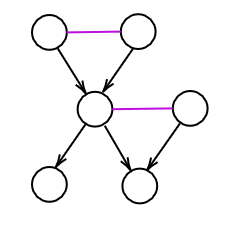
\includegraphics[width=0.2\textwidth]{Figs/a19.png}
    \caption{}
    % \label{fig:zcvdnjf}
\end{figure}
\end{proof}
\begin{rema}
In \cref{eq:nefa} we define  Markov blanket for one distribution. Here we define  Markov blanket for a graph, i.e. all the distributions that factors over graph.
\end{rema}

 Intuitively, moralization causes loss of information about independencies only when it introduces new edges (add edges between parents) into the graph. However, in special cases
 \begin{defa}\bfs{Moral}
 We say that a Bayesian network $\mathcal{G}$ is \tb{moral} if it contains no immoralities (as in \cref{def:immor}); that is, for any pair of variables $X, Y$ that share a child, there is a covering edge between $X$ and $Y$. 
 \end{defa}
 \begin{thma}\bfs{Moralized Graph is perfect I-map for Moral DAG}\label{thm:hddad}
 If the directed graph $\mathcal{G}$ is moral, then its moralized graph $\mathcal{M}[\mathcal{G}]$ is a \tb{perfect map} of $\mathcal{G}$.
 \end{thma}
\begin{proof}
Let $\mathcal{H}=\mathcal{M}[\mathcal{G}]$. We have already shown that $\mathcal{I}(\mathcal{H}) \subseteq \mathcal{I}(\mathcal{G})$, so it remains to show the opposite inclusion. Assume by contradiction that there is an independence $(\boldsymbol{X} \perp \boldsymbol{Y} \mid \boldsymbol{Z}) \in$ $\mathcal{I}(\mathcal{G})$ which is not in $\mathcal{I}(\mathcal{H})$. Thus, in $\calH$, there must exist some trail from $\boldsymbol{X}$ to $\boldsymbol{Y}$ in $\mathcal{H}$ which is active given $\boldsymbol{Z}$. Consider some such trail that is minimal, in the sense that it has no shortcuts. As $\mathcal{H}$ and $\mathcal{G}$ have precisely the same edges, the same trail must exist in $\mathcal{G}$. As, by assumption, it cannot be active in $\mathcal{G}$ given $\boldsymbol{Z}$, we conclude that it must contain a $v$-structure $X_{1} \rightarrow X_{2} \leftarrow X_{3}$. However, because $\mathcal{G}$ is moralized, we also have some edge between $X_{1}$ and $X_{3}$, contradicting the assumption that the trail is minimal.
\end{proof}
\begin{rema}
 Thus, a moral graph $\mathcal{G}$ can be converted to a Markov network without losing independence assumptions.  We note, however, that very few directed graphs are moral. For example, assume that we have a v-structure $X \rightarrow Y \leftarrow Z$, which is moral due to the existence of an arc $X \rightarrow Z$. If $Z$ has another parent $W$, it also has a v-structure $X \rightarrow Z \leftarrow W$, which, to be moral, requires some edge between $X$ and $W$. Such cases are rare.
\end{rema}
\paragraph{Soundness of d-Separation*}\label{sec:meqkdka}
The connection between Bayesian networks and Markov networks provides us with the tools for proving the soundness of the d-separation criterion in Bayesian networks. The idea behind the proof is to leverage the soundness of separation in undirected graphs.

Thus, we want to construct an undirected graph $\mathcal{H}$ such that active paths in $\mathcal{H}$ correspond to active paths in $\mathcal{G}$. However if we use the moralized graph directly, there are paths in the undirected graph that correspond to $v$-structures in $\mathcal{G}$ that may or may not be active. For example, if our graph $\mathcal{G}$ is $X \rightarrow Z \leftarrow Y$ and $Z$ is not observed, d-separation tells us that $X$ and $Y$ are independent; but the moralized graph for $\mathcal{G}$ is the complete undirected graph, which does not have the same independence.

\begin{defa}\bfs{Barren Nodes}
Let $\mathcal{B}=(\mathcal{G}, P)$ be a Bayesian network over some set of variables $\mathcal{X}$. Consider some subset of evidence nodes $\boldsymbol{Z}$, and let $\boldsymbol{X}$ be all of the ancestors of the nodes in $\boldsymbol{Z}$. Let $\mathcal{B}^{\prime}$ be a network over the induced subgraph over $\boldsymbol{X}$, where the CPD for every node $X \in \boldsymbol{X}$ is the same in $\mathcal{B}^{\prime}$ as in $\mathcal{B}$. The joint distribution over $\boldsymbol{X}$ is the same in $\mathcal{B}$ and in $\mathcal{B}^{\prime}$. The nodes in $\mathcal{X}-\boldsymbol{X}$ are called \tb{barren nodes relative to $\boldsymbol{X}$,} because (when not instantiated) they are irrelevant to computations concerning $\boldsymbol{X}$.
\end{defa}



\tb{Recall \cref{def:dnmfa} of upward closure }: We let $\mathcal{G}^{+}[\boldsymbol{U}]$ be the induced Bayesian network over $\boldsymbol{U}$ and its ancestors, i.e. the upward closure of $\boldsymbol{U}$.
\begin{rema}%\bfs{}
Other nodes are \tb{barren nodes}. The elimination of the barren nodes does not change the independence properties of the distribution over the remaining variables, but does eliminate paths in the graph involving $v$-structures that are not friendly. If we now consider only the subgraph, we can reduce d-separation to separation and utilize the soundness of separation to show the desired result.
\end{rema}

\begin{lema}\label{lem:kdkjf}
 Let $\boldsymbol{X}, \boldsymbol{Y}, \boldsymbol{Z}$ be three disjoint sets of nodes in a Bayesian network $\mathcal{G}$. Let $\boldsymbol{U}=\boldsymbol{X} \cup \boldsymbol{Y} \cup \boldsymbol{Z}$, and let $\mathcal{G}^{\prime}=\mathcal{G}^{+}[\boldsymbol{U}]$ be the induced Bayesian network graph over $\boldsymbol{U} \cup\mathrm{Ancestors}_{\boldsymbol{U}}$. Let $\mathcal{H}$ be the moralized graph $\mathcal{M}\left[\mathcal{G}^{\prime}\right] .$ Then $\text{$\mathrm{d}$-$\mathrm{sep}$}_{\mathcal{G}}(\boldsymbol{X} ; \boldsymbol{Y} \mid \boldsymbol{Z})$ if and only if $\operatorname{sep}_{\mathcal{H}}(\boldsymbol{X} ; \boldsymbol{Y} \mid \boldsymbol{Z}) .$ 
\end{lema}
\begin{proof}
If there exist an active path in $\calG$, for (a),(b),(c) cases in \cref{fig:3node}, we can find a same path in $\calH$. For (d) the $v$-structure in the path, shortcut exists in $\calH$, so there exist an active path is $\calH$.

If there exists an active path in $\calH$, still only $v$-structure in $\calG$ without covering edge matters. For the connection between the two parents, we have two cases in $\calG$:
\begin{enumerate}
    \item The $v$-structure has the observed middle node or its observed descendants in $\boldsymbol{Z}$, the $v$-structure is active, we just replace the connection between the two parents with the middle node in $\calG$.
    \item If a $v$-structure does not satisfies this but still be included in $\mathcal{G}^{\prime}$, this only is possible that the $v$-structure has middle node or its descendants  in $(\boldsymbol{X}\cup\boldsymbol{Y})$ but not in $(\boldsymbol{Z}$, we then have another guaranteed connection between the middle node (or its descendants) to the original path two ends (the two ends one is in $\boldsymbol{X}$ and one is in $\boldsymbol{Y}$). We therefore find an active path in $\calG$.
\end{enumerate}
(Anther way to prove: for each pair $X\in\boldsymbol{X}$ and $Y\in\boldsymbol{Y}$, we construct the upward closure of $X\cup Y\cup\boldsymbol{Z}$. It is more clear that now $v$-structure need to be active and avoid discuss case 2.)
\end{proof}
Recall {D-separation and Independence I}  \cref{thm:dsep1}:
\begin{thma}
If a distribution $P_{\calB}$ factorizes according to $\mathcal{G}$, then $\mathcal{G}$ is an I-map for $P_{\calB}$, i.e. $\mathcal{I}(\mathcal{G}) \subseteq \mathcal{I}(P_{\calB})$.
\end{thma}
\begin{proof}
Let $\boldsymbol{U}=\boldsymbol{X} \cup \boldsymbol{Y} \cup \boldsymbol{Z}$, let $\boldsymbol{U}^{*}=\boldsymbol{U} \cup$ Ancestors $_{\boldsymbol{U}}$, let $\mathcal{G}_{\boldsymbol{U}^{*}}=\mathcal{G}^{+}[\boldsymbol{U}]$ be the induced graph over $\boldsymbol{U}^{*}$, and let $\mathcal{H}$ be the moralized graph $\mathcal{M}\left[\mathcal{G}_{\boldsymbol{U}^{*}}\right]$. Let $P_{U^{*}}$ be the Bayesian network distribution defined over $\mathcal{G}_{U^{*}}$ in the obvious way: the CPD for any variable in $\boldsymbol{U}^{*}$ is the same as in $\mathcal{B}$. Because $\boldsymbol{U}^{*}$ is upwardly closed, all variables used in these CPDs are in $\boldsymbol{U}^{*}$.

Now, consider an independence assertion $(\boldsymbol{X} \perp \boldsymbol{Y} \mid \boldsymbol{Z}) \in \mathcal{I}(\mathcal{G})$; we want to prove that $P_{\calB} \models(\boldsymbol{X} \perp \boldsymbol{Y} \mid \boldsymbol{Z}) .$ Since $(\boldsymbol{X} \perp \boldsymbol{Y} \mid \boldsymbol{Z}) \in \mathcal{I}(\mathcal{G})$, we have that $\text{$\mathrm{d}$-$\mathrm{sep}$}_{\mathcal{G}}(\boldsymbol{X} ; \boldsymbol{Y} \mid$ $\boldsymbol{Z})$. It follows that $\operatorname{sep}_{\mathcal{H}}(\boldsymbol{X} ; \boldsymbol{Y} \mid \boldsymbol{Z})$, and hence that $(\boldsymbol{X} \perp \boldsymbol{Y} \mid \boldsymbol{Z}) \in \mathcal{I}(\mathcal{H})$.  $P_{\boldsymbol{U}^{*}}$ is a Gibbs distribution over $\mathcal{H}$, and hence, from \cref{thm:sep1}, $P_{\boldsymbol{U}^{*}} \models(\boldsymbol{X} \perp \boldsymbol{Y} \mid \boldsymbol{Z})$. The distribution $P_{\boldsymbol{U}^{*}}\left(\boldsymbol{U}^{*}\right)$ is the same as $P_{\calB}\left(\boldsymbol{U}^{*}\right) .$ Hence, it follows also that $P_{\calB} \models(\boldsymbol{X} \perp \boldsymbol{Y} \mid \boldsymbol{Z})$, proving the desired result.
\end{proof} 


\subsubsection{From Markov Networks to Bayesian Networks}
We now consider the converse transformation: finding a Bayesian network that is a minimal I-map for a Markov network. It turns out that the transformation in this direction is significantly more difficult, both conceptually and computationally. Indeed, the Bayesian network that is a minimal I-map for a Markov network need have more edges:  \tb{it has no immoralities and must be chordal.}
\begin{exma}
\begin{figure}[H]
    \centering
    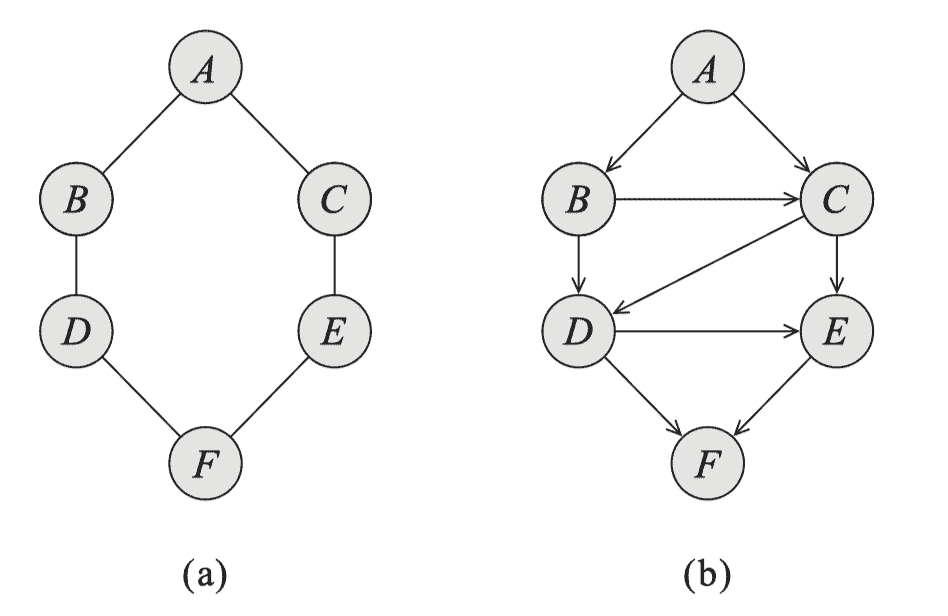
\includegraphics[width=0.6\textwidth]{Figs/a20.png}
    \caption{Minimal I-map Bayesian networks for a nonchordal Markov network.
(a) A Markov network $\mathcal{H}_{\ell}$ with a loop. (b) A minimal I-map $\mathcal{G}_{\ell}$ Bayesian network for $\mathcal{H}$.}
    \label{fig:zcvdnjf}
\end{figure}
Consider the Markov network structure $\mathcal{H}_{\ell}$ of \cref{fig:zcvdnjf} (a), and assume that we want to find a Bayesian network I-map for $\mathcal{H}_{\ell}$. As we discussed in \cref{sec:jhdsddq}, we can find such an I-map by enumerating the nodes in $\mathcal{X}$ in some ordering, and define the parent set for each one in turn according to the independencies in the distribution. Assume we enumerate the nodes in the order $A, B, C, D, E, F$. The process for $A$ and $B$ is obvious. Consider what happens when we add $C$. We must, of course, introduce $A$ as a parent for $C$. More interestingly, however, $C$ is not independent of $B$ given $A$; hence, we must also add $B$ as a parent for $C$. Now, consider the node $D$. One of its parents must be $B$. As $D$ is not independent of $C$ given $B$, we must add $C$ as a parent for $B$. We do not need to add $A$, as $D$ is independent of $A$ given $B$ and $C$. Similarly, E's parents must be $C$ and $D$. Overall, the minimal Bayesian network I-map according to this ordering has the structure $\mathcal{G}_{\ell}$ shown in \cref{fig:zcvdnjf} (b).
\end{exma}
\begin{rema}
It shows that we have added several edges to the graph, resulting in a set of triangles crisscrossing the loop. In fact, the graph $\mathcal{G}_{\ell}$ in \cref{fig:zcvdnjf} (b) is \tb{chordal}: all loops have been partitioned into triangles.  This phenomenon is a general one, see \cref{cor:ajdc}). 
\end{rema}
In fact, we can show the following property, which is even stronger:
\begin{thma}
Let $\mathcal{H}$ be a Markov network structure, and let $\mathcal{G}$ be any Bayesian network minimal I-map for $\mathcal{H}$. Then $\mathcal{G}$ can have \tb{no immoralities.}
\end{thma}
\begin{proof}
 Let $X_{1}, \ldots, X_{n}$ be a topological ordering for $\mathcal{G}$. Assume, by contradiction, that there is some immorality $X_{i} \rightarrow X_{j} \leftarrow X_{k}$ in $\mathcal{G}$ such that there is no edge between $X_{i}$ and $X_{k}$; assume (without loss of generality) that $i<k<j$.
\begin{figure}[H]
    \centering
    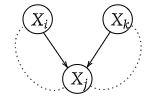
\includegraphics[width=0.3\textwidth]{Figs/a13.png}
    % \caption{}
    % \label{fig:zcvdnjf}
    \end{figure}
Owing to minimality of the constructed I-map $\mathcal{G}$, $\mathcal{H}$ necessarily contains one or more paths between $X_{i}$ and $X_{j}$ that are not cut by $X_{k}$ (or by $X_{j}$'s other parents). Otherwise, there is no connection of $X_i-X_{j}$ in the construction.
Similarly, $\mathcal{H}$ necessarily contains one or more paths between $X_{k}$ and $X_{j}$ that are not cut by $X_{i}$ (or by $X_{j}$'s other parents).

Consider the parent set $\boldsymbol{U}$ that was chosen for $X_{k}$. By our previous argument, there are one or more paths in $\mathcal{H}$ between $X_{i}$ and $X_{k}$ via $X_{j}$. As $i<k$, and $X_{i}$ is not a parent of $X_{k}$ (by our assumption), we have that \tb{$\boldsymbol{U}$ must cut all of those paths.} To do so, $\boldsymbol{U}$ must cut either all of the paths between $X_{i}$ and $X_{j}$, or all of the paths between $X_{j}$ and $X_{k}$ : As long as there is at least one active path from $X_{i}$ to $X_{j}$ and one from $X_{j}$ to $X_{k}$, there is an active path between $X_{i}$ and $X_{k}$ that is not cut by $\boldsymbol{U}$. Assume, without loss of generality, that \tb{$\boldsymbol{U}$ cuts all paths between $X_{j}$ and $X_{k}$} (the other case is symmetrical).

Now, consider the choice of parent set for $X_{j}$, and recall that it is the (unique) minimal subset among $X_{1}, \ldots, X_{j-1}$ that separates $X_{j}$ from the others. In a Markov network, this set consists of all nodes in $X_{1}, \ldots, X_{j-1}$ that are the first on some uncut path from $X_{j} .$ As \tb{$\boldsymbol{U}$ separates $X_{k}$ from $X_{j}$}, it follows that $X_{k}$ cannot be the first on any uncut path from $X_{j}$, and therefore $X_{k}$ cannot be a parent of $X_{j} .$ This result provides the desired contradiction.
\end{proof}

\begin{cora}\label{cor:ajdc}
Let $\mathcal{H}$ be a Markov network structure, and let $\mathcal{G}$ be any minimal $I$-map for $\mathcal{H} .$ \tb{Then $\mathcal{G}$ is necessarily chordal.}
\end{cora}
\begin{proof}
Because any nontriangulated loop of length at least 4 in a Bayesian network graph necessarily contains an immorality. 
\begin{figure}[H]
    \centering
    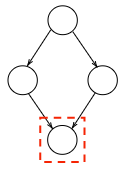
\includegraphics[width=0.2\textwidth]{Figs/a14.png}
    % \caption{}
    % \label{fig:zcvdnjf}
    \end{figure}
\end{proof}
\begin{defa}\bfs{Triangulation}
Thus, the process of turning a Markov network into a Bayesian network requires that we \tb{add enough edges to a graph to make it chordal.} This process is called \tb{triangulation}. 
\end{defa}
\begin{rema}
As in the transformation from Bayesian networks to Markov networks, the addition of edges leads to the loss of independence information. 
\end{rema}
\subsubsection{Chordal Graphs and Clique Tree}
\tb{Question: } When a set of independence assumptions can be represented perfectly by both a Bayesian network and a Markov network.

\tb{Answer: } This class is precisely the class of \tb{undirected chordal graphs.}

\tb{Summary: }
\begin{enumerate}
    \item \tb{$\mathcal{I}(\mathcal{H})=\mathcal{I}(\mathcal{G})\Rightarrow$  $\calH$ is chordal}: see \cref{thm:atere}
    \item \tb{ $\exists \calH$ s.t. $\mathcal{I}(\mathcal{H})=\mathcal{I}(\mathcal{G})\Leftarrow$ chordal $\calH$:} see \cref{thm:adfadf}
\end{enumerate}


\begin{thma}\label{thm:atere}
Let $\mathcal{H}$ be a \tb{nonchordal} Markov network. Then there is no Bayesian network $\mathcal{G}$ which is a perfect map for $\mathcal{H}$ (that is, such that $\mathcal{I}(\mathcal{H})=\mathcal{I}(\mathcal{G})$).
\end{thma}
\begin{proof}
It follows from the fact that the minimal I-map for $\mathcal{G}$ must be chordal.
\end{proof}


To prove the other direction of this equivalence, we first prove some important properties of chordal graphs. As we will see, \tb{chordal graphs and the properties we now show play a central role in the derivation of exact inference algorithms for graphical models.} 

For the remainder of this discussion, we restrict attention to \tb{connected graphs}; the extension to the general case is straightforward: use a set of connected graphs and a set of  tree, i.e. forest.


$\bullet$ \tb{Goal: }{\tb{decompose chordal graph $\mathcal{H}$ into clique tree}}


\tb{Some notation:} Let $\mathcal{H}$ be a connected undirected graph, and let $\boldsymbol{C}_{1}, \ldots, \boldsymbol{C}_{k}$ be the set of maximal cliques in $\mathcal{H}$. 
\begin{enumerate}
    \item Let $\mathcal{T}$ be any tree-structured graph whose nodes correspond to the maximal cliques $\boldsymbol{C}_{1}, \ldots, \boldsymbol{C}_{k}$:
    \begin{defa}\bfs{Sepset}
    Let $\boldsymbol{C}_{i}, \boldsymbol{C}_{j}$ be two cliques in the tree that are directly connected by an edge; we define $\boldsymbol{S}_{i, j}=\boldsymbol{C}_{i} \cap \boldsymbol{C}_{j}$ to be a \tb{sepset} between $\boldsymbol{C}_{i}$ and $\boldsymbol{C}_{j} .$
    \end{defa}
    \item Let $\boldsymbol{W}_{<(i, j)}\left(\boldsymbol{W}_{<(j, i)}\right)$ be all of the variables that appear in any clique on the $\boldsymbol{C}_{i}$ $\left(\boldsymbol{C}_{j}\right)$ side of the edge. Thus, each edge decomposes $\mathcal{X}$ into three disjoint sets:
\begin{enumerate}
    \item $\boldsymbol{W}_{<(i, j)}-\boldsymbol{S}_{i, j}$,
    \item  $\boldsymbol{W}_{<(j, i)}-\boldsymbol{S}_{i, j}$, and
    \item  $\boldsymbol{S}_{i, j}$
\end{enumerate} 
\end{enumerate}
\begin{figure}[H]
    \centering
    
\includegraphics[width=0.6\textwidth]{Figs/a22.png}
    % \caption{}
    % \label{fig:zcvdnjf}
\end{figure}

\begin{defa}\bfs{Clique Tree}
We say that \tb{a tree $\mathcal{T}$ is a clique tree for $\mathcal{H}$} if:
\begin{enumerate}
    \item  each node corresponds to a clique in $\mathcal{H}$, and each maximal clique in $\mathcal{H}$ is a node in $\mathcal{T}$;
    \item each sepset $\boldsymbol{S}_{i, j}$ \tb{separates} $\boldsymbol{W}_{<(i, j)}$ and $\boldsymbol{W}_{<(j, i)}$ in $\mathcal{H}$. (so only one path)
\end{enumerate}
\end{defa}
\begin{rema}
Note that this definition implies that \tb{each separator $\boldsymbol{S}_{i, j}$ renders its two sides conditionally independent in $\mathcal{H}$}.
\end{rema}

\begin{thma}\label{thm:fdaxv}
Every undirected chordal graph $\mathcal{H}$ has a clique tree $\mathcal{T}$.
\end{thma}
\begin{proof}
We prove the theorem by induction on the number of nodes in the graph. The base case of a single node is trivial. Now, consider a chordal graph $\mathcal{H}$ of size $>1$. If $\mathcal{H}$ consists of a single clique, then the theorem holds trivially. Therefore, consider the case where we have at least two nodes $X_{1}, X_{2}$ that are not connected directly by an edge, i.e. not a single clique. 

Let $\boldsymbol{S}$ be a minimal subset of nodes that separates $X_{1}$ and $X_{2}$. The removal of the set $\boldsymbol{S}$ breaks up the graph into \tb{two disconnected components} (if $>2$, the other connected components can be assigned to the below $\boldsymbol{W}_{1}$ or $\boldsymbol{W}_{2}$ arbitrarily)
\begin{enumerate}
    \item Let $\boldsymbol{W}_{1}$ be one partition of the variables in $\mathcal{X}-\boldsymbol{S}$ containing $X_{1}$.
    \item Let  $\boldsymbol{W}_{2}$ be the other partition of the variables in $\mathcal{X}-\boldsymbol{S}$ containing $X_{2}$.
    \item $\boldsymbol{W}_{1}\cup\boldsymbol{W}_{2}=\mathcal{X}-\boldsymbol{S}$ and  $\boldsymbol{W}_{1}\cap\boldsymbol{W}_{2}=\emptyset$.
\end{enumerate}

 $\diamond$ \tb{We first show that $\boldsymbol{S}$ must be a complete subgraph}. 
 
 Let $Z_{1}, Z_{2}$ be any two variables in $\boldsymbol{S}$. Due to the minimality of $\boldsymbol{S}$, each $Z_{i}$ must lie on a path between $X_{1}$ and $X_{2}$ that does not go through any other node in $\boldsymbol{S}$. (Otherwise, we could eliminate $Z_{i}$ from $\boldsymbol{S}$ while still maintaining separation.)
 \begin{figure}[H]
    \centering
    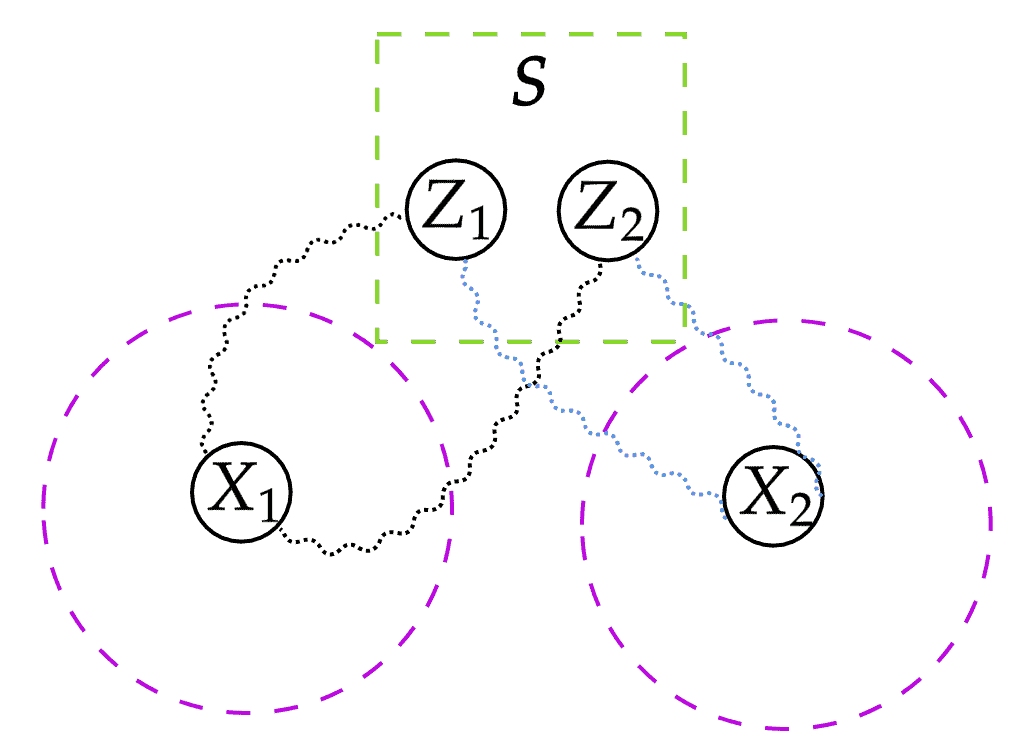
\includegraphics[width=0.6\textwidth]{Figs/a23.png}
    % \caption{}
    % \label{fig:zcvdnjf}
\end{figure}
 We can therefore construct a minimal path from $Z_{1}$ to $Z_{2}$ that goes only through nodes in $\boldsymbol{W}_{1}$ by constructing a path from $Z_{1}$ to $X_{1}$ to $Z_{2}$ that goes only through $\boldsymbol{W}_{1}$, and then \tb{eliminating any shortcuts}. We can similarly construct a minimal path from $Z_{1}$ to $Z_{2}$ that goes only through nodes in $\boldsymbol{W}_{2}$. The two paths together form a cycle of length $\geq 4 .$ Because of chordality, the cycle must have a chord, which, by construction, must be the edge $Z_{1}-Z_{2}$.

$\diamond$ \tb{Construct a tree  $\calT$ with nodes being cliques.}

Now consider the induced graph $\mathcal{H}_{1}=\mathcal{H}\left[\boldsymbol{W}_{1} \cup \boldsymbol{S}\right] .$ As $X_{2} \notin \mathcal{H}_{1}$, this induced graph is smaller than $\mathcal{H} .$ Moreover, $\mathcal{H}_{1}$ is chordal, so we can apply the inductive hypothesis. Let $\mathcal{T}_{1}$ be the clique tree for $\mathcal{H}_{1}$. Because $\boldsymbol{S}$ is a complete connected subgraph, it is either a maximal clique or a subset of some maximal clique in $\mathcal{H}_{1}$. Let $\boldsymbol{C}_{1}$ be some clique in $\mathcal{T}_{1}$ containing $\boldsymbol{S}$ (there may be more than one such clique). We can similarly define $\mathcal{H}_{2}$ and $\boldsymbol{C}_{2}$ for $X_{2} .$ 
\begin{enumerate}
    \item If neither $\boldsymbol{C}_{1}$ nor $\boldsymbol{C}_{2}$ is equal to $\boldsymbol{S}$, we construct a tree $\mathcal{T}$ that contains the union of the cliques in $\mathcal{T}_{1}$ and $\mathcal{T}_{2}$, and connects $\boldsymbol{C}_{1}$ and $\boldsymbol{C}_{2}$ by an edge. 
    \item Otherwise, without loss of generality, let $\boldsymbol{C}_{1}=\boldsymbol{S} ;$ we create $\mathcal{T}$ by merging $\mathcal{T}_{1}$ minus $\boldsymbol{C}_{1}$ into $\mathcal{T}_{2}$, making all of $\boldsymbol{C}_{1}$'s neighbors adjacent to $\boldsymbol{C}_{2}$ instead.
\end{enumerate}

$\diamond$ \tb{Prove $\calT$ a clique tree for $\mathcal{H}$}

\tb{Step 1 prove maximal:} We note that there is no clique in $\mathcal{H}$ that intersects both $W_{1}$ and $W_{2}$ since otherwise $\boldsymbol{W}_1$ and $\boldsymbol{W}_2$ have connected path. Hence, any maximal clique in $\mathcal{H}$ is a maximal clique in either $\mathcal{H}_{1}$ or $\mathcal{H}_{2}$ (or both in the possible case of $\boldsymbol{S}$ ), so that {all maximal cliques in $\mathcal{H}$ appear in $\mathcal{T}$}. 
Thus, the nodes in $\mathcal{T}$ are precisely the maximal cliques in $\mathcal{H}$. 

\tb{Step 2 prove separation:} We need to show that any $\boldsymbol{S}_{i, j}$ separates $\boldsymbol{W}_{<(i, j)}$ and $\boldsymbol{W}_{<(j, i)} .$  Consider two variables $X \in \boldsymbol{W}_{<(i, j)}$ and $Y \in \boldsymbol{W}_{<(j, i)} .$ 
\begin{enumerate}
    \item First, assume that $X, Y \in \mathcal{H}_{1}$; as all the nodes in $\mathcal{H}_{1}$ are on the $\mathcal{T}_{1}$ side of the tree, we also have that $\boldsymbol{S}_{i, j} \subset \mathcal{H}_{1}$. Any path between two nodes in $\mathcal{H}_{1}$ that goes through $\boldsymbol{W}_{2}$ can be shortcut to go only through $\mathcal{H}_{1}$. Thus, if $\boldsymbol{S}_{i, j}$ separates $X, Y$ in $\mathcal{H}_{1}$, then it also separates them in $\mathcal{H}$. The same argument applies for $X, Y \in \mathcal{H}_{2}$.
    \item Now, consider $X \in \boldsymbol{W}_{1}$ and $Y \in \boldsymbol{W}_{2}$. If $\boldsymbol{S}_{i, j}\supseteq\boldsymbol{S}$, the result follows from the fact that $\boldsymbol{S}$ separates $\boldsymbol{W}_{1}$ and $\boldsymbol{W}_{2}$. Otherwise, assume that $\boldsymbol{S}_{i, j}$ is in $\mathcal{T}_{1}$, on the path from $X$ to $\boldsymbol{C}_{1}$.
    % $X$ must in $W_1-S_i,j. S \subet S_ij$, so $Sij$ block the way of $X$ to $S$.
    In this case, we have that $\boldsymbol{S}_{i, j}$ separates $X$ from $\boldsymbol{S}$, and $\boldsymbol{S}$ separates $\boldsymbol{S}_{i, j}$ from $Y$. The conclusion now follows from the transitivity of graph separation.
\end{enumerate} 
We have therefore constructed a clique tree for $\mathcal{H}$, proving the inductive claim.
\end{proof}
\begin{thma}\label{thm:adfadf}
Let $\mathcal{H}$ be a chordal Markov network. Then there is a Bayesian network $\mathcal{G}$ such that $\mathcal{I}(\mathcal{H})=\mathcal{I}(\mathcal{G})$.
\end{thma}
\begin{proof}
Let $\mathcal{T}$ be the clique tree for $\mathcal{H}$, whose existence is guaranteed by \cref{thm:fdaxv}. We can select an ordering over the nodes in the Bayesian network as follows:
\begin{enumerate}
    \item \tb{Clique ordering:} We first select an arbitrary clique $\boldsymbol{C}_{1}$ to be the root of the clique tree, and then order the cliques $\boldsymbol{C}_{1}, \ldots, \boldsymbol{C}_{k}$ using any topological ordering, such that cliques closer to the root are ordered first.
\item \tb{Variable ordering:} We then order the nodes in the network in any ordering consistent with the clique ordering: if $X_{l}$ first appears in $\boldsymbol{C}_{i}$ and $X_{m}$ first appears in $\boldsymbol{C}_{j}$, for $i<j$, then $X_{l}$ must precede $X_{m}$ in the ordering.
\end{enumerate}  We now construct a Bayesian network using the procedure Build-Minimal-I-Map in \cref{fig:imapminimal} applied to the resulting node ordering $X_{1}, \ldots, X_{n}$ using $\mathcal{I}(\mathcal{H})$.

Let $\mathcal{G}$ be the resulting network. We first show that, when $X_{i}$ is added to the graph, then $X_{i}$'s parents are precisely $\boldsymbol{U}_{i}\coloneqq\mathrm{Nb}_{X_{i}} \cap\left\{X_{1}, \ldots, X_{i-1}\right\}$, where $\mathrm{Nb}_{X_{i}}$ is the set of neighbors of $X_{i}$ in $\mathcal{H}$. So we need to show that $X_{i}$ is independent of $\left\{X_{1}, \ldots, X_{i-1}\right\}-\boldsymbol{U}_{i}$ given $\boldsymbol{U}_{i}$.

Let $\boldsymbol{C}_{k}$ be the first clique in the clique ordering to which $X_{i}$ belongs.  Let $\boldsymbol{C}_{l}$ be the parent of $\boldsymbol{C}_{k}$ in the rooted clique tree. We then have $X_i\notin \boldsymbol{C}_l$. Also none of $\{X_{1}, \ldots, X_{i-1}\}$ belongs to the  descendants of $\boldsymbol{C}_{k}$ in the clique tree. So we have given $\boldsymbol{S}_{l,k}=\boldsymbol{C}_{l}\cap \boldsymbol{C}_{k}$,  $\{X_{1}, \ldots, X_{i-1}\}-\boldsymbol{S}_{l,k}$ are a subset of $\boldsymbol{W}_{<(l, k)}$. $X_i\in \boldsymbol{W}_{>(l, k)}$. We then have that   $X_{i}$ is independent of all of $\left\{X_{1}, \ldots, X_{i-1}\right\}-\boldsymbol{S}_{l,k}$ given $\boldsymbol{S}_{l,k}$. But note that $\boldsymbol{S}_{l,k}\subseteq\{X_{1}, \ldots, X_{i-1}\}$ since $\boldsymbol{S}_{l,k}\subseteq\boldsymbol{C}_l$ so each element should be already presented in $\{X_{1}, \ldots, X_{i-1}\}$. Also note that $\boldsymbol{S}_{l,k}\subseteq\boldsymbol{C}_l$, a clique, so $X_i$ is connected to each node in $\boldsymbol{S}_{l,k}$ that means $\boldsymbol{S}_{l,k}\subseteq\mathrm{Nb}_{X_i}$. We so have $\boldsymbol{S}_{l,k}\subseteq\mathrm{Nb}_{X_{i}} \cap\left\{X_{1}, \ldots, X_{i-1}\right\}$. If one node in $\mathrm{Nb}_{X_{i}} \cap\left\{X_{1}, \ldots, X_{i-1}\right\}$ is not in $\boldsymbol{S}_{l,k}$, we cannot have the conditional independent. So the minimal $\boldsymbol{U}_i=\boldsymbol{S}_{l,k}=\mathrm{Nb}_{X_{i}} \cap\left\{X_{1}, \ldots, X_{i-1}\right\}$.

 It follows that $\mathcal{G}$ and $\mathcal{H}$ have the same set of edges. Moreover, we note that all of $\boldsymbol{U}_{i}$ are in $\boldsymbol{C}_{k}$, and hence are connected in $\mathcal{G}$. (Please think in iterated way) Therefore, $\mathcal{G}$ is moralized. As $\mathcal{H}$ is the moralized undirected graph of $\mathcal{G}$, the result now follows from \cref{thm:hddad}.
\end{proof}


\subsubsection{Summary}
\begin{figure}[H]
    \centering
    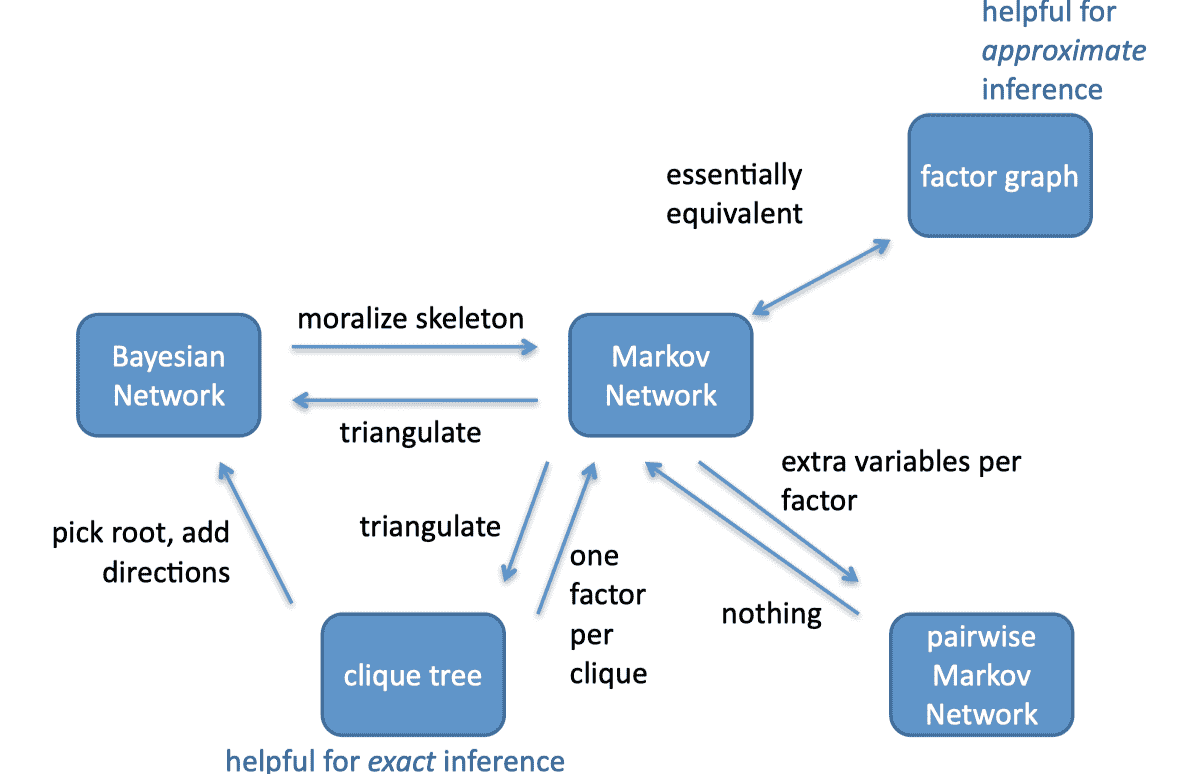
\includegraphics[width=0.8\textwidth]{Figs/a21.png}
    % \caption{}
    % \label{fig:zcvdnjf}
\end{figure}
\subsection{Partially Directed Models: A Unify of DAG and Undirected Model}
We can unify both representations by allowing models that incorporate both directed and undirected dependencies.
We first introduce conditional random field, a Markov network with a directed dependency on some subset of variables. It is can be viewed as  partially directed models\cref{sec:oasdjcn}. We then present a generalization of this framework to the class of chain graphs, an entire network in which undirected components depend on each other in a directed fashion.
\subsubsection{Conditional Random Fields}\label{sec:crf}
So far, we have described the Markov network representation as encoding a joint distribution over $\mathcal{X}$. The same undirected graph representation and parameterization can also be used to encode a conditional distribution $P(\boldsymbol{Y} \mid \boldsymbol{X})$, where $\boldsymbol{Y}$ is a set of \tb{target variables} and $\boldsymbol{X}$ is a (disjoint) set of \tb{observed variables.}
\paragraph{CRF Representation}
\begin{defa}\bfs{Conditional Random Field}\label{def:crf}
A \tb{conditional random field} is an undirected graph $\mathcal{H}$ whose nodes correspond to $\boldsymbol{X} \cup \boldsymbol{Y}$; the network is annotated with a set of factors $\phi_{1}\left(\boldsymbol{D}_{1}\right), \ldots, \phi_{m}\left(\boldsymbol{D}_{m}\right)$ such that each $\boldsymbol{D}_{i} \not \subseteq \boldsymbol{X}$. The network encodes a conditional distribution as follows:
\begin{align}
\begin{aligned}
P(\boldsymbol{Y} \mid \boldsymbol{X}) &=\frac{1}{Z(\boldsymbol{X})} \tilde{P}(\boldsymbol{Y}, \boldsymbol{X}) \\
\tilde{P}(\boldsymbol{Y}, \boldsymbol{X}) &=\prod_{i=1}^{m} \phi_{i}\left(\boldsymbol{D}_{i}\right) \\
Z(\boldsymbol{X}) &=\sum_{\boldsymbol{Y}} \tilde{P}(\boldsymbol{Y}, \boldsymbol{X})
\end{aligned}\label{eq:dfaeea}
\end{align}
Two variables in $\mathcal{H}$ are connected by an (undirected) edge whenever they appear together in the scope of some factor.
\end{defa}
\begin{rema}\bfs{explanation}
 To have the network structure and parameterization correspond naturally to a conditional distribution given observed variables, \tb{we disallow potentials that involve only variables in $\boldsymbol{X}$.} The only difference between \cref{eq:dfaeea} and the (unconditional) Gibbs distribution of \cref{def:xzda} is the different normalization used in the partition function $Z(\boldsymbol{X})$. The definition of a CRF induces a different value for the partition function for every assignment $\boldsymbol{x}$ to $\boldsymbol{X}$. 
\end{rema}
\begin{exma}\label{ex:mdnfa}
\begin{figure}[H]
    \centering
    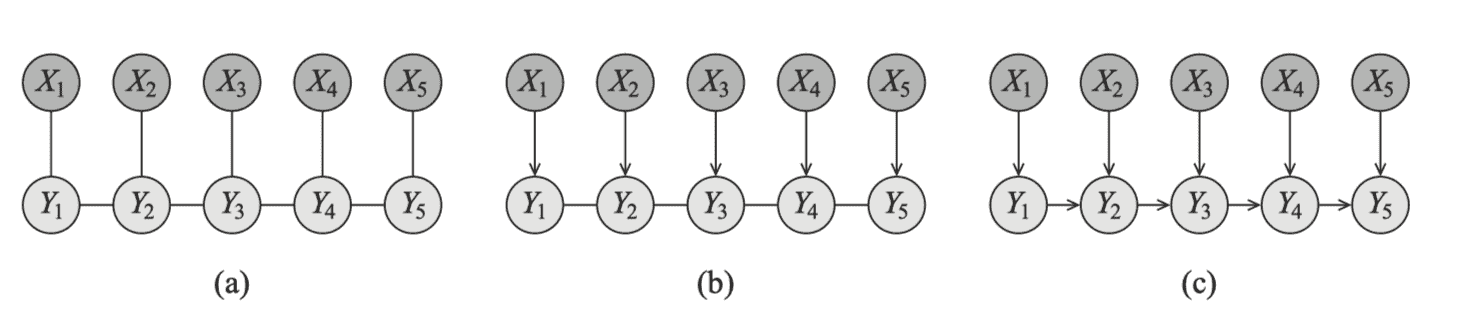
\includegraphics[width=0.8\textwidth]{Figs/a24.png}
    \caption{Different linear-chain graphical models: (a) a linear-chain-structured conditional random field, where the feature variables are denoted using grayed-out ovals; (b) a partially directed variant; (c) a fully directed, non-equivalent model. The $X_i$'s are assumed to be always observed when the network is used, and hence they are shown as darker gray.}
    \label{fig:oerkla}
\end{figure}
Consider a CRF over $\boldsymbol{Y}=\left\{Y_{1}, \ldots, Y_{k}\right\}$ and $\boldsymbol{X}=\left\{X_{1}, \ldots, X_{k}\right\}$, with an edge $Y_{i}-Y_{i+1}$ $(i=1, \ldots, k-1)$ and an edge $Y_{i}-X_{i}(i=1, \ldots, k)$, as shown in \cref{fig:oerkla} (a). The distribution represented by this network has the form:
\begin{align*}
\begin{aligned}
P(\boldsymbol{Y} \mid \boldsymbol{X}) &=\frac{1}{Z(\boldsymbol{X})} \tilde{P}(\boldsymbol{Y}, \boldsymbol{X}) \\
\tilde{P}(\boldsymbol{Y}, \boldsymbol{X}) &=\prod_{i=1}^{k-1} \phi\left(Y_{i}, Y_{i+1}\right) \prod_{i=1}^{k} \phi\left(Y_{i}, X_{i}\right) \\
Z(\boldsymbol{X}) &=\sum_{\boldsymbol{Y}} \tilde{P}(\boldsymbol{Y}, \boldsymbol{X})
\end{aligned}
\end{align*}
\end{exma}
$\bullet$ \tb{More Explanation:}
\begin{enumerate}
    \item \tb{Edges in $\boldsymbol{X}$:} The structure of a CRF may still contain edges between variables in $\boldsymbol{X}$, which arise when two such variables appear together in a factor that also contains a target variable. However, edges in $\boldsymbol{X}$ \tb{do not encode the structure of any distribution over $\boldsymbol{X}$,} since the network explicitly does not encode any such distribution.
    \item \tb{Why avoid encoding the distribution over the variables in $X$?} This flexibility allows us to incorporate into the model a rich set of observed variables whose dependencies may be quite complex or even poorly understood. It also allows us to include continuous variables whose distribution may not have a simple parametric form. This flexibility allows us to use domain knowledge in order to define a rich set of features characterizing our domain, without worrying about modeling their joint distribution. 
\end{enumerate}
\begin{exma}
For example, returning to the vision MRFs \cref{ex:mdfe}, rather than defining a joint distribution over pixel values and their region assignment, we can define a conditional distribution over segment assignments given the pixel values. The use of a conditional distribution here allows us to avoid making a parametric assumption over the (continuous) pixel values. Even more important, we can use image-processing routines to define rich features, such as the presence or direction of an image gradient at a pixel. Such features can be highly informative in determining the region assignment of a pixel. \tb{However, the definition of such features usually relies on multiple pixels, and defining a correct joint distribution or a set of independence assumptions over these features is far from trivial.} The fact that we can condition on these features and avoid this whole issue allows us the flexibility to include them in the model. 
\end{exma}
 

\paragraph{Directed and Undirected Dependencies}\label{sec:oasdjcn}

A CRF defines a conditional distribution of $\boldsymbol{Y}$ on $\boldsymbol{X}$; thus, it can be viewed as a \tb{partially directed graph, where we have an undirected component over $Y$, which has the variables in $\boldsymbol{X}$ as parents.}
\begin{exma}\bfs{naive Markov model}
Consider a CRF over the binary-valued variables $\boldsymbol{X}=\left\{X_{1}, \ldots, X_{k}\right\}$ and $\boldsymbol{Y}=\{Y\}$, and a pairwise potential between $Y$ and each $X_{i}$. Assume that the pairwise potentials defined via the following log-linear model
\begin{align*}
\phi_{i}\left(X_{i}, Y\right)=\exp \left\{w_{i} \mathbf{I}\left\{X_{i}=1, Y=1\right\}\right\} .
\end{align*}
We also introduce a single-node potential $\phi_{0}(Y)=\exp \left\{w_{0} \mathbb{I}\{Y=1\}\right\}$. Following \cref{eq:dfaeea},
we now have:
\begin{align*}
\begin{aligned}
\tilde{P}\left(Y=1 \mid x_{1}, \ldots, x_{k}\right) &=\exp \left\{w_{0}+\sum_{i=1}^{k} w_{i} x_{i}\right\} \\
\tilde{P}\left(Y=0 \mid x_{1}, \ldots, x_{k}\right) &=\exp \{0\}=1
\end{aligned}
\end{align*}
In this case, we can show that
\begin{align*}
P\left(Y=1 \mid x_{1}, \ldots, x_{k}\right)=\operatorname{sigmoid}\left(w_{0}+\sum_{i=1}^{k} w_{i} x_{i}\right)
\end{align*}
where
\begin{align*}
\operatorname{sigmoid}(z)=\frac{e^{z}}{1+e^{z}}.
\end{align*}
is the sigmoid function. This conditional distribution $P(Y \mid \boldsymbol{X})$ is of great practical interest: It defines a CPD that is not structured as a table, but that is induced by a small set of parameters $w_{0}, \ldots, w_{k}$ - parameters whose number is linear, rather than exponential, in the number of parents. This type of CPD is  called a \tb{logistic CPD.}
\end{exma}
\begin{exma}
The partially directed model for the CRF of \cref{ex:mdnfa} is shown in \cref{fig:oerkla} (b). The fully directed attempt, such as the one in \cref{fig:oerkla} (c), is not correct. 
\end{exma}
\subsubsection{Chain Graph Models}
We now present a more general framework that builds on the CRF representation and can be used to provide a general treatment of the independence assumptions made in these partially directed models. 

\tb{Recall PDAG \cref{def:cadfe}:}  the nodes can be disjointly partitioned into several chain components. An edge between two nodes in the same chain component must be \tb{undirected}, while an edge between two nodes in different chain components must be \tb{directed}. Thus, PDAGs are also called chain graphs.
\paragraph{Factorization}
For a PDAG $\mathcal{K}$, intuitively, the factorization for PDAGs represents the distribution as a product of each of the chain components given its parents. Thus, we call such a representation a \tb{chain graph model.}

% Intuitively, each chain component $\boldsymbol{K}_{i}$ in the chain graph model is associated with a CRF that defines $\mathcal{P}\left(\boldsymbol{K}_{i} \mid \mathrm{Pa}_{\boldsymbol{K}_{i}}\right)$ - the conditional distribution of $\boldsymbol{K}_{i}$ given its parents in the graph. More precisely, each is defined via a set of factors that involve the variables in $\boldsymbol{K}_{i}$ and their parents; the distribution $\mathcal{P}\left(\boldsymbol{K}_{i} \mid \mathrm{Pa}_{\boldsymbol{K}_{i}}\right)$ is defined by using the factors associated with $\boldsymbol{K}_{i}$ to define a CRF whose target variables are $\boldsymbol{K}_{i}$ and whose observable variables are $\mathrm{Pa}_{\boldsymbol{K}_{i}}$.

To provide a formal definition, it helps to introduce the concept of a moralized PDAG.
\begin{defa}\bfs{Moralized Graph}
Let $\mathcal{K}$ be a PDAG and $\boldsymbol{K}_{1}, \ldots, \boldsymbol{K}_{\ell}$ be its chain components. We define $\mathrm{Pa}_{\boldsymbol{K}_{i}}$ to be the \tb{set of parents} for \tb{nodes in $\boldsymbol{K}_{i}$}. The \tb{moralized graph} of $\mathcal{K}$ is an \tb{undirected graph $\mathcal{M}[\mathcal{K}]$} produced by first connecting, using undirected edges, any pair of nodes $X, Y \in \mathrm{Pa}_{K_{i}}$ for all $i=1, \ldots, \ell$, and then converting all directed edges into undirected edges.
\end{defa}
\begin{rema}\bfs{special case: directed graph}
 This definition generalizes our earlier notion of a moralized directed graph. In the case of directed graphs, each node is its own chain component, and hence we are simply adding undirected edges between the parents of each node.
\end{rema}

\begin{exma}
\begin{figure}[H]
    \centering
    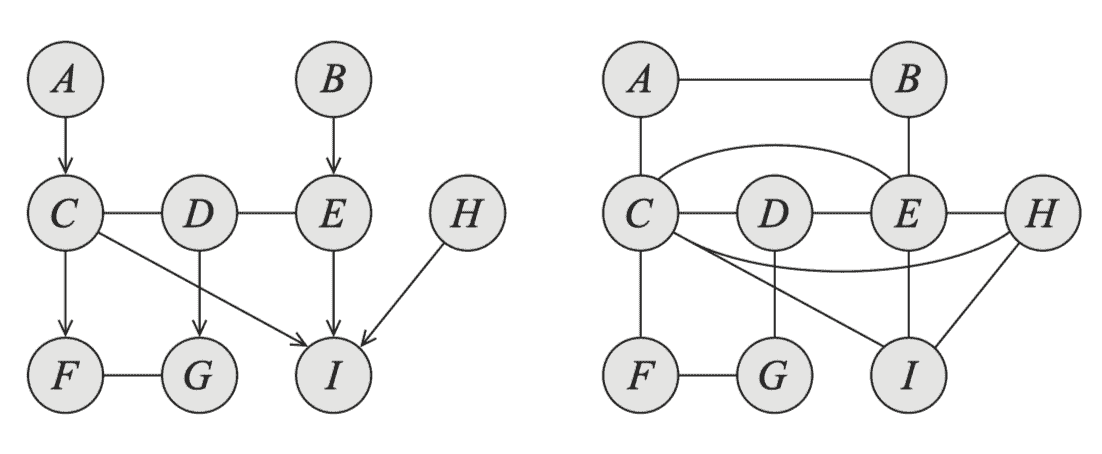
\includegraphics[width=0.5\textwidth]{Figs/a25.png}
    \caption{A chain graph $\calK$ and its moralized version}
    \label{fig:avfbf}
\end{figure}
\cref{fig:avfbf} shows a chain graph and its moral graph. We have added the edge between $A$ and $B$, since they are both parents of the chain component $\{C, D, E\}$, and edges between $C, E$, and $H$, because they are parents of the chain component $\{I\}$. Note that we did not add an edge between $D$ and $H$ (even though $D$ and $C, E$ are in the same chain component), since $D$ is not a parent of I.
\end{exma}


We can now define the factorization of a chain graph:
\begin{defa}\bfs{Chain Graph Distribution; Factorization}
Let $\mathcal{K}$ be a PDAG, and $\boldsymbol{K}_{1}, \ldots, \boldsymbol{K}_{\ell}$ be its chain components. A chain graph distribution is defined via a set of factors $\phi_{i}\left(\boldsymbol{D}_{i}\right)(i=1, \ldots, m)$, where each $\boldsymbol{D}_{i}$ is a \tb{complete subgraph} in the moralized graph $\mathcal{M}\left[\mathcal{K}\right]$  such that 
\begin{enumerate}
    \item $\boldsymbol{D}_{i} \subseteq \boldsymbol{K}_{i} \cup \mathrm{Pa}_{\boldsymbol{K}_{i}}$, $\boldsymbol{D}_{i} \not \subseteq \mathrm{Pa}_{\boldsymbol{K}_{i}}$
    \item $\phi_{i}\left(\boldsymbol{D}_{i}\right)$ is associated with a single chain component $\boldsymbol{K}_{j}$,
    \item We then define $P\left(\boldsymbol{K}_{i} \mid \mathrm{Pa}_{\boldsymbol{K}_{i}}\right)$ as a CRF as in \cref{def:crf} with these factors, and with $\boldsymbol{Y}_{i}=\boldsymbol{K}_{i}$ and $\boldsymbol{X}_{i}=\mathrm{Pa}_{\boldsymbol{K}_{i}}$. 
\end{enumerate}   We now define
\begin{align*}
P(\mathcal{X})=\prod_{i=1}^{\ell} P\left(\boldsymbol{K}_{i} \mid \mathrm{Pa}_{\boldsymbol{K}_{i}}\right) .
\end{align*}
We say that a distribution $P$ \tb{factorizes} over $\mathcal{K}$ if it can be represented as a chain graph distribution over $\mathcal{K}$.
\end{defa}
% \begin{rema}\bfs{explanation}
%  $\mathcal{M}\left[\mathcal{K}^{+}\left[\boldsymbol{D}_{i}\right]\right]$. 
% \end{rema}

\begin{exma}
In the chain graph model defined by the graph of \cref{fig:avfbf}, we require that the conditional distribution $P(C, D, E \mid A, B)$ factorize according to the graph of \cref{fig:dlal} (a). Specifically, we would have to define the conditional probability as a normalized product of factors:
\begin{align*}
\frac{1}{Z(A, B)} \phi_{1}(A, C) \phi_{2}(B, E) \phi_{3}(C, D) \phi_{4}(D, E) .
\end{align*}
A similar factorization applies to $P(F, G \mid C, D)$.
\end{exma}

\paragraph{Independencies in Chain Graphs}
As for undirected graphs, there are \tb{three distinct interpretations} for the independence properties induced by a PDAG. 

\tb{Recall some definitions \cref{def:cadfe}:} 
\begin{enumerate}
    \item \tb{Boundary:} We define $\mathrm{Boundary}_{X}$ to be $\mathrm{Pa}_{X} \cup \mathrm{Nb}_{X}$;
    \item $\mathrm{Descendants}_{X}$: $X$'s descendants. For each node in $\mathrm{Descendants}_{X}$, there exists a \tb{directed path}, i.e. at least one directed edge, $X_{1}, \ldots, X_{k}$ with $X_{1}=X$ and $X_{k}=$ the node. 
    % \item 
\end{enumerate}
Thus, in the case of PDAGs, it follows that if $Y$ is a descendant of $X$, then $Y$ must be in a "lower" chain component.
\begin{defa}\bfs{Pairwise Independencies}
For a PDAG $\mathcal{K}$, we define the pairwise independencies associated with $\mathcal{K}$ to be:
\begin{align*}
\begin{gathered}
\mathcal{I}_{p}(\mathcal{K})=\left\{\left(X \perp Y \mid\left(\mathrm{NonDescendants}_{X}-\{X, Y\}\right)\right):\right. \\
\left.X, Y \text { non-adjacent }, Y \in \mathrm{NonDescendants}_{X}\right\} .
\end{gathered}
\end{align*}
\end{defa}
\begin{rema}
 This definition generalizes the pairwise independencies for undirected graphs: 
 \begin{enumerate}
     \item in an undirected graph, nodes have no descendants, so  $\mathrm{NonDescendants}_{X}=\mathcal{X}$.
     \item Similarly, it is not too hard to show that these independencies also hold in a directed graph.
 \end{enumerate} 
\end{rema}
\begin{defa}\bfs{Local Independencies }
For a PDAG $\mathcal{K}$, we define the local independencies associated with $\mathcal{K}$ to be:
\begin{align*}
\mathcal{I}_{\ell}(\mathcal{K})=\left\{\left(X \perp \mathrm{NonDescendants}_{X}-\mathrm{Boundary}_{X} \mid \mathrm{Boundary}_{X}\right): X \in \mathcal{X}\right\} .
\end{align*}
\end{defa}
\begin{rema}
This definition generalizes the definition of local independencies for both directed and undirected graphs.
\begin{enumerate}
    \item For directed graphs,  $\mathrm{NonDescendants}_{X}$ is precisely the set of nondescendants, whereas  $\mathrm{Boundary}_{X}$ is the set of parents.
    \item For undirected graphs,  $\mathrm{NonDescendants}_{X}$ is $\mathcal{X}$, whereas  $\mathrm{Boundary}_{X}=\mathrm{Nb}_{X}$.
\end{enumerate} 
\end{rema}
We define the global independencies in a PDAG using the definition of moral graph. Our definition follows the lines of \cref{lem:kdkjf}.
\begin{defa}\bfs{c-separation}
Let $\boldsymbol{X}, \boldsymbol{Y}, \boldsymbol{Z} \subset \mathcal{X}$ be three disjoint sets, and let $\boldsymbol{U}=\boldsymbol{X} \cup \boldsymbol{Y} \cup \boldsymbol{Z}$. We say that $\boldsymbol{X}$ is c-separated from $\boldsymbol{Y}$ given $\boldsymbol{Z}$ if $\boldsymbol{X}$ is separated from $\boldsymbol{Y}$ given $\boldsymbol{Z}$ in the undirected graph $\mathcal{M}\left[\mathcal{K}^{+}[\boldsymbol{X} \cup \boldsymbol{Y} \cup \boldsymbol{Z}]\right] .$
\end{defa}
\begin{exma}
\begin{figure}[H]
    \centering
    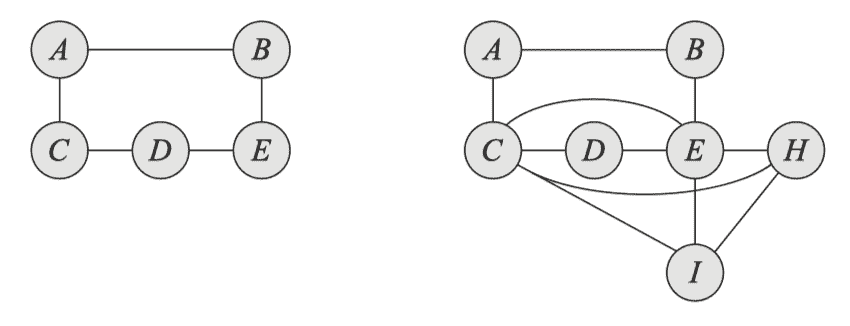
\includegraphics[width=0.5\textwidth]{Figs/a26.png}
    \caption{ Example for definition of c-separation in a chain graph. (a) The Markov network $\mathcal{M}\left[\mathcal{K}^{+}[C, D, E]\right]$. (b) The Markov network $\mathcal{M}\left[\mathcal{K}^{+}[C, D, E, I]\right]$.}
    \label{fig:dlal}
\end{figure}
Consider again the PDAG of \cref{fig:avfbf}. Then $C$ is $c$-separated from $E$ given $D, A$, because $C$ and $E$ are separated given $D, A$ in the undirected graph $\mathcal{M}\left[\mathcal{K}^{+}[\{C, D, E\}]\right]$, shown in \cref{fig:dlal} (a). However, $C$ is not c-separated from $E$ given only $D$, since there is a path between $C$ and $E$ via $A, B$. On the other hand, $C$ is not separated from $E$ given $D, A, I$. The graph $\mathcal{M}\left[\mathcal{K}^{+}[\{C, D, E, I\}]\right]$ is shown in \cref{fig:dlal} (b). As we can see, the introduction of $I$ into the set $\boldsymbol{U}$ causes us to introduce a direct edge between $C$ and $E$ in order to moralize the graph. Thus, we cannot block the path between $C$ and $E$ using $D, A, I$.
\end{exma}
\begin{rema}
\begin{rema}This definition generalizes the definition for both directed and undirected graphs.
\begin{enumerate}
    \item This notion of c-separation clearly generalizes the notion of separation in undirected graphs, since the ancestors of a set $\boldsymbol{U}$ in an undirected graph are simply the entire set of nodes $\mathcal{X}$.
    \item It also generalizes the notion of d-separation in directed graphs, using the equivalent definition provided in proposition \cref{lem:kdkjf}.
\end{enumerate}
\end{rema}
\end{rema}
  Using the definition of c-separation, we can finally define the notion of global Markov independencies:
  \begin{defa}\bfs{global independencies}
  Let $\mathcal{K}$ be a PDAG. We define the global independencies associated with $\mathcal{K}$  to be:
\begin{align*}
\mathcal{I}(\mathcal{K})=\{(\boldsymbol{X} \perp \boldsymbol{Y} \mid \boldsymbol{Z}): \boldsymbol{X}, \boldsymbol{Y}, \boldsymbol{Z} \subset \mathcal{X}, \boldsymbol{X} \text { is c-separated from } \boldsymbol{Y} \text { given } \boldsymbol{Z}\} .
\end{align*}
  \end{defa}

As in the case of undirected models, these three criteria for independence are not equivalent for nonpositive distributions. The inclusions are the same: the global independencies imply the local independencies, which in turn imply the pairwise independencies. Because undirected models are a subclass of PDAGs, the same counterexamples used for undirected graph show that the inclusions are strict for nonpositive distributions. \tb{For positive distributions, we again have that the three definitions are equivalent.}



We note that, as in the case of Bayesian networks, the parents of a chain component are always \tb{fully connected} in $\mathcal{M}\left[\mathcal{K}\left[\boldsymbol{K}_{i} \cup \mathrm{Pa}_{\boldsymbol{K}_{i}}\right]\right]$. Thus, while the structure over the parents helps factorize the distribution over the chain components containing the parents, it does not give rise to independence assertions in the conditional distribution over the child chain component. Importantly, however, it does give rise to structure in the form of the parameterization of $P\left(\boldsymbol{K}_{i} \mid \operatorname{Pa}_{\boldsymbol{K}_{i}}\right)$.

As in the case of directed and undirected models, we have an equivalence between the requirement of factorization of a distribution and the requirement that it satisfy the independencies associated with the graph. Not surprisingly, since PDAGs generalize undirected graphs, this equivalence only holds for positive distributions:
\begin{thma}
A positive distribution $P$ factorizes over a $P D A G \mathcal{K}$ if and only if $P \models \mathcal{I}(\mathcal{K})$.
\end{thma}
\begin{proof}
We omit the proof.
\end{proof}


\section{The Exponential Family and Entropy}
\subsection{Exponential Families}
 We now consider parametric  families of distributions. We will be interested in families that can be written in a particular form.
\begin{defa}\bfs{Exponential Family}
Let $\mathcal{X}$ be a set of variables. An exponential family $\mathcal{P}$ over $\mathcal{X}$ is specified by four components:
\begin{itemize}
    \item  A \tb{sufficient statistics function} $\tau$ from assignments to $\mathcal{X}$ to $\mathcal{R}^{K}$.
    \item A \tb{parameter space} that is a \tb{convex set} $\Theta \subseteq \mathcal{R}^{M}$ of legal parameters.
    \item A \tb{natural parameter function} $\mathrm{t}$ from $\mathcal{R}^{M}$ to $R^{K}$.
    \item An \tb{auxiliary measure} $A$ over $\mathcal{X}$.
\end{itemize}
Each vector of parameters $\theta \in \Theta$ specifies a distribution $P_{\theta}$ in the family as
\begin{align*}
P_{\boldsymbol{\theta}}(\xi)=\frac{1}{Z(\boldsymbol{\theta})} A(\xi) \exp \{\langle\mathrm{t}(\boldsymbol{\theta}), \tau(\xi)\rangle\}
\end{align*}
where $\langle\mathrm{t}(\boldsymbol{\theta}), \tau(\xi)\rangle$ is the inner product of the vectors $\mathrm{t}(\boldsymbol{\theta})$ and $\tau(\xi)$, and
\begin{align*}
Z(\boldsymbol{\theta})=\sum_{\xi} A(\xi) \exp \{\langle\mathrm{t}(\boldsymbol{\theta}), \tau(\xi)\rangle\}
\end{align*}
is the \tb{partition function} of $\mathcal{P}$, which must be \tb{finite}. The parametric family $\mathcal{P}$ is defined as:
\begin{align*}
\mathcal{P}=\left\{P_{\boldsymbol{\theta}}: \boldsymbol{\theta} \in \Theta\right\} .
\end{align*}
\end{defa}
\begin{defa}\bfs{explanation}
The sufficient statistic function $\tau$ summarizes the aspects of an instance that are relevant for assigning it a probability. If $A$ is a constant, level set of $\tau$ has the same probability.  The function $t$ maps the parameters to space of the range of sufficient statistics.  In most of the examples we consider here $A$ is a constant, and we will mention it explicitly only when it is not a constant.
\end{defa}
\begin{exma}\bfs{Bernoulli Distribution}\label{ex:dfafdyrq}
Consider a simple Bernoulli distribution. To show that this distribution is in the exponential family, we can set
\begin{align*}
\tau(X)=\left\langle\ \indicate{X=x^{1}}, \indicate{X=x^{0}}\right\rangle
\end{align*}
a numerical vector representation of the value of $X$, and
\begin{align*}
\mathrm{t}(\theta)=\langle\ln \theta, \ln (1-\theta)\rangle .
\end{align*}
It is easy to see that for $X=x^{1}$, we have $\tau(X)=\langle 1,0\rangle$, and thus
\begin{align*}
\exp \{\langle\mathrm{t}(\theta), \tau(X)\rangle\}=e^{1 \cdot \ln \theta+0 \cdot \ln (1-\theta)}=\theta \text {. }
\end{align*}
Similarly, for $X=x^{0}$, we get that $\exp \{\langle\mathrm{t}(\theta), \tau(X)\rangle\}=1-\theta$. We conclude that, by setting $Z(\theta)=1$, this representation is identical to the Bernoulli distribution.
\end{exma}
\begin{exma}\bfs{Gaussian Distribution}
Consider a Gaussian distribution over a single variable. Recall that
\begin{align*}
P(x)=\frac{1}{\sqrt{2 \pi} \sigma} \exp \left\{-\frac{(x-\mu)^{2}}{2 \sigma^{2}}\right\} .
\end{align*}
Define
\begin{align*}
\begin{aligned}
\tau(x) &=\left\langle x, x^{2}\right\rangle \\
\mathrm{t}\left(\mu, \sigma^{2}\right) &=\left\langle\frac{\mu}{\sigma^{2}},-\frac{1}{2 \sigma^{2}}\right\rangle \\
Z\left(\mu, \sigma^{2}\right) &=\sqrt{2 \pi} \sigma \exp \left\{\frac{\mu^{2}}{2 \sigma^{2}}\right\}
\end{aligned}
\end{align*}
We can easily verify that
\begin{align*}
P(x)=\frac{1}{Z\left(\mu, \sigma^{2}\right)} \exp \{\langle\mathrm{t}(\theta), \tau(X)\rangle\} .
\end{align*}
\end{exma}
$\bullet$ In many cases, we set some requirements
\begin{enumerate}
    \item We want the parameter space $\Theta$ to to be a \tb{convex, open subset} of $\mathcal{R}^{M}$. 
    \item We want $\boldsymbol{\theta} \neq \boldsymbol{\theta}^{\prime}$ to imply $P_{\boldsymbol{\theta}} \neq P_{\boldsymbol{\theta}^{\prime}}$, i.e., \tb{the function $t$ is invertible (over the set $\Theta$ )}.  We call such exponential families are \tb{invertible} or \tb{nonredundant}. 
\end{enumerate}
These desiderata help us execute certain operations effectively, in particular, finding a distribution $Q$ in some exponential family that is a "good approximation" to some other distribution $P$.
\subsection{Linear Exponential Families}
Linear exponential families discussed here is the canonical exponential families in ``Mathematical Statistics Notes''. Parameters are also called the \tb{natural parameters} for the given sufficient statistic function. 
We have 
\begin{align*}
P_{\boldsymbol{\theta}}(\xi)=\frac{1}{Z(\boldsymbol{\theta})} \exp \{\langle\boldsymbol{\theta}, \tau(\xi)\rangle\} .
\end{align*}
\begin{defa}\bfs{Natural Parameter Space}
More generally, when we consider natural parameters for a sufficient statistics function $\tau$, we define the set of allowable natural parameters, the \tb{natural parameter space}, to be the set of natural parameters that can be normalized
\begin{align*}
\Theta=\left\{\boldsymbol{\theta} \in \mathcal{R}^{K}: \int \exp \{\langle\boldsymbol{\theta}, \tau(\xi)\rangle\} d \xi<\infty\right\} .
\end{align*}
\end{defa}
\begin{rema}
In the case of distributions over \tb{finite discrete spaces}, all parameter choices lead to normalizable distributions, and so $\Theta=\mathcal{R}^{K}$.
\end{rema}
 
 \begin{defa}\bfs{Linear Exponential Family}
 An exponential family over the natural parameter space, and for which the natural parameter space is \tb{open and convex}, is called a linear exponential family.
 \end{defa}

In some examples we may provide an alternative parameterization of a nonlinear exponential family as a linear exponential family
\begin{exma}\bfs{Gaussian Distribution}
Consider again the Gaussian distribution. Suppose we define a new parameter space using the definition of $\mathrm{t}$. That is let $\boldsymbol{\eta}=\mathrm{t}\left(\mu, \sigma^{2}\right)=\left\langle\frac{2 \mu}{2 \sigma^{2}},-\frac{1}{2 \sigma^{2}}\right\rangle$ be the natural parameters that corresponds to $\boldsymbol{\theta}=\left\langle\mu, \sigma^{2}\right\rangle$. Clearly, we can now write
\begin{align*}
P_{\boldsymbol{\eta}}(x) \propto \exp \{\langle\boldsymbol{\eta}, \tau(x)\rangle\} .
\end{align*}
However, not every choice of $\boldsymbol{\eta}$ would lead to a legal distribution. For the distribution to be normalized, we need to be able to compute
\begin{align*}
\begin{aligned}
Z(\boldsymbol{\eta}) &=\int \exp \{\langle\boldsymbol{\eta}, \tau(x)\rangle\} d x \\
&=\int_{-\infty}^{\infty} \exp \left\{\eta_{1} x+\eta_{2} x^{2}\right\} d x
\end{aligned}
\end{align*}
If $\eta_{2} \geq 0$ this integral is undefined, since the function grows when $x$ approaches $\infty$ and $-\infty .$ When $\eta_{2}<0$, the integral has a finite value. Fortunately, if we consider $\boldsymbol{\eta}=\mathrm{t}\left(\mu, \sigma^{2}\right)$, we see that the second component is always negative (since $\sigma^{2}>0$ ). In fact, we can see that the image of the original parameter space, $\left\langle\mu, \sigma^{2}\right\rangle \in \mathcal{R} \times \mathcal{R}^{+}$, through the function $\mathrm{t}\left(\mu, \sigma^{2}\right)$, is the space $\mathcal{R} \times \mathcal{R}^{-}$. We can verify that, for every $\boldsymbol{\eta}$ in that space, the normalization constant is well defined.
\end{exma}
\begin{exma}\bfs{Bernoulli Distribution}
The formulation in \cref{ex:dfafdyrq} is redundant. However, we can use reparameter technique in ``{Multinomial Trials in Mathematical Statistics Notes}'' to get nonredundant linear  exponential family:
\begin{align*}
\begin{aligned}
\tau(x) &=\indicate{x=x^{1}} \\
\mathrm{t}(\theta) &=\ln \frac{\theta}{1-\theta}
\end{aligned}
\end{align*}
We see that
\begin{align*}
\begin{aligned}
\exp \left\{\left\langle\mathrm{t}(\theta), \tau\left(x^{1}\right)\right\rangle\right\} &=\frac{\theta}{1-\theta} \\
\exp \left\{\left\langle\mathrm{t}(\theta), \tau\left(x^{0}\right)\right\rangle\right\} &=1
\end{aligned}
\end{align*}
Thus,
\begin{align*}
Z(\theta)=1+\frac{\theta}{1-\theta}=\frac{1}{1-\theta} .
\end{align*}
Using these, we can verify that
\begin{align*}
P_{\theta}\left(x^{1}\right)=(1-\theta) \frac{\theta}{1-\theta}=\theta \text {. }
\end{align*}
We conclude that this exponential representation captures the Bernoulli distribution. Notice now that, in the new representation, the \tb{image of $\mathrm{t}$ is the whole real line $\mathcal{R}$.} Thus, we can define a \tb{linear} exponential family with this sufficient statistic function.
\end{exma}
\tb{Question:} Are there exist families that are not linear?

\tb{Answer:} Yes. In ``Mathematical Statistics Notes'', we introduce curved exponential families, which cannot be converted to linear. See also next section.

\subsection{Factored Exponential Families}
\subsubsection{Log-linear Models }
In \cref{def:loglinear}, we defined \tb{log-linear models} as distributions of the form:
\begin{align*}
P\left(X_{1}, \ldots, X_{n}\right) \propto \exp \left\{\sum_{i=1}^{k} \theta_{i} \cdot f_{i}\left(\boldsymbol{D}_{i}\right)\right\}
\end{align*}
where each feature $f_{i}$ is a function whose scope is $\boldsymbol{D}_{i}$. 
Such a distribution is clearly a \tb{linear exponential family} where the \tb{sufficient statistics} are the vector of features
\begin{align*}
\tau(\xi)=\left\langle f_{1}\left(\boldsymbol{d}_{1}\right), \ldots, f_{k}\left(\boldsymbol{d}_{k}\right)\right\rangle
\end{align*}
\begin{rema}
Note \tb{discrete Markov networks are linear exponential families} since we can devise a log-linear model to represent a given discrete Markov network structure.
\end{rema}
\subsubsection{Product Distributions}
What about other distributions with product forms? A product form of terms corresponds to a simple composition of exponential families
\begin{defa}\bfs{Exponential Factor Family}
An (unnormalized) \tb{exponential factor family} $\Phi$ is defined by $\tau, \mathrm{t}, A$, and $\Theta$ (as in the exponential family). A factor in this family is
\begin{align*}
\phi_{\boldsymbol{\theta}}(\xi)=A(\xi) \exp \{\langle\mathrm{t}(\boldsymbol{\theta}), \tau(\xi)\rangle\} .
\end{align*}
\end{defa}
\begin{defa}\bfs{Family Composition}
Let $\Phi_{1}, \ldots, \Phi_{k}$ be exponential factor families, where each $\Phi_{i}$ is specified by $\tau_{i}, \mathrm{t}_{i}, A_{i}$, and $\Theta_{i}$. The \tb{composition} of $\Phi_{1}, \ldots, \Phi_{k}$ is the family $\Phi_{1} \times \Phi_{2} \times \cdots \times \Phi_{k}$ parameterized by $\boldsymbol{\theta}=$ $\boldsymbol{\theta}_{1} \circ \boldsymbol{\theta}_{2} \circ \cdots \circ \boldsymbol{\theta}_{k} \in \Theta_{1} \times \Theta_{2} \times \cdots \times \Theta_{k}$, defined as
\begin{align*}
P_{\boldsymbol{\theta}}(\xi) \propto \prod_{i} \phi_{\boldsymbol{\theta}_{i}}(\xi)=\left(\prod_{i} A_{i}(\xi)\right) \exp \left\{\sum_{i}\left\langle\mathrm{t}_{i}\left(\boldsymbol{\theta}_{i}\right), \tau_{i}(\xi)\right\rangle\right\}
\end{align*}
where $\phi_{\boldsymbol{\theta}_{i}}$ is a factor in the i'th factor family. The composition of exponential factors is an exponential family with
\begin{enumerate}
    \item $\tau(\xi)=\tau_{1}(\xi) \circ \tau_{2}(\xi) \circ \cdots \circ \tau_{k}(\xi)$ and 
    \item natural parameters $\mathrm{t}(\boldsymbol{\theta})=\mathrm{t}_{1}\left(\boldsymbol{\theta}_{1}\right) \circ \mathrm{t}_{2}\left(\boldsymbol{\theta}_{2}\right) \circ$ $\cdots \circ \mathrm{t}_{k}\left(\boldsymbol{\theta}_{k}\right)$.
\end{enumerate}
\end{defa}
\begin{rema}
Moreover, it follows that the \tb{product of linear exponential factor families is a linear exponential family.}
\end{rema}
\begin{rema}
We ignored the partition functions of the individual factors, allowing the partition function of the overall distribution to ensure global normalization.
\end{rema}
\subsubsection{Bayesian Networks}
As we have discussed in \cref{sec:qmadfd}, a parameterized Bayesian network with a set of CPD can be viewed as a set of factors with additional normalization constraints. If we have a set of CPDs from an exponential family, then their product is also in the exponential family. Thus, we can conclude that \tb{a Bayesian network with exponential CPDs defines an exponential family.}
\paragraph{Exponential CPDs}
$\bullet$ \tb{Discrete:}

Clearly, we get the exponential form for any CPD for discrete variables. 
\begin{exma}
We start by examining a simple discrete table-CPD $P(X \mid \boldsymbol{U})$. Similar to the case of Bernoulli distribution, we can define the sufficient statistics to be indicators for different entries in $P(X \mid \boldsymbol{U})$. Thus, we set
\begin{align*}
\tau_{P(X \mid \boldsymbol{U})}(\mathcal{X})=\langle\indicate{X=x, \boldsymbol{U}=\boldsymbol{u}}: x \in \mathrm{Val}(X), \boldsymbol{u} \in \mathrm{Val}(\boldsymbol{U})\rangle
\end{align*}
We set the natural parameters to be the corresponding parameters
\begin{align*}
\mathrm{t}_{P(X \mid \boldsymbol{U})}(\boldsymbol{\theta})=\langle\ln P(x \mid \boldsymbol{u}): x \in \mathrm{Val}(X), \boldsymbol{u} \in \mathrm{Val}(\boldsymbol{U})\rangle
\end{align*}
It is easy to verify that
\begin{align*}
P(x \mid \boldsymbol{u})=\exp \left\{\left\langle\mathrm{t}_{P(X \mid \boldsymbol{U})}(\boldsymbol{\theta}), \tau_{P(X \mid \boldsymbol{U})}(x, \boldsymbol{u})\right\rangle\right\}
\end{align*}
since exactly one entry of $\tau_{P(X \mid \boldsymbol{U})}(x, \boldsymbol{u})$ is 1 and the rest are $0$. Note that this representation is not a linear exponential factor since we have $\ln$.
\end{exma}

$\bullet$ \tb{Continuous:}

For continuous CPDs, not every CPD can be represented by an exponential factor. However, some cases can.
\begin{exma}
Consider a linear Gaussian CPD for $P(X \mid \boldsymbol{U})$ where
\begin{align*}
X=\beta_{0}+\beta_{1} u_{1}+\cdots+\beta_{k} u_{k}+\epsilon
\end{align*}
where $\epsilon$ is a Gaussian random variable with mean 0 and variance $\sigma^{2}$, representing the noise in the system. Stated differently, the conditional density function of $X$ is
\begin{align*}
P(x \mid \boldsymbol{u})=\frac{1}{\sqrt{2 \pi} \sigma} \exp \left\{-\frac{1}{2 \sigma^{2}}\left(x-\left(\beta_{0}+\beta_{1} u_{1}+\cdots+\beta_{k} u_{k}\right)\right)^{2}\right\}
\end{align*}

By expanding the squared term, we find that the \tb{sufficient statistics} are the first and second moments of all the variables
\begin{align}
\tau_{P(X \mid \boldsymbol{U})}(\mathcal{X})=\left\langle 1, x, u_{1}, \ldots, u_{k}, x^{2}, x u_{1}, \ldots, x u_{k}, u_{1}^{2}, u_{1} u_{2}, \ldots, u_{k}^{2}\right\rangle\label{eq:dfad}
\end{align}
and the \tb{natural parameters} (it is linear exponential family) are the coefficients of each of these terms.
\end{exma}

$\bullet$  \tb{Some explanation:}

In the above two examples, we construct a \tb{normalized conditional distribution.} This allows us to use the chain rule to compose these factors into a joint distribution without the requirement of a partition function. This requirement turns out to be critical: \tb{We cannot construct a Bayesian network from a product of unnormalized exponential factors.}

\tb{Question:} {Why?}

\tb{Answer: } {The global normalization constant cannot play the role of a local normalization constant within each conditional distribution. This implies that to have an exponential representation of a Bayesian network, we need to ensure that each CPD is \tb{locally normalized}.}
\begin{rema}
For every exponential CPD this is easy to do. We simply increase the dimension of $\tau$ by adding another dimension that has a constant value, say $1 .$ Then the matching element of $t(\theta)$ can be the logarithm of the partition function. See \cref{eq:dfad}.
\end{rema}

\begin{exma}
Consider the network structure $A \rightarrow B$, with binary variables. We consider defining
\begin{align*}
\tau(A, B)=\left\langle \indicate{A=a^{1}}, \indicate{B=b^{1}, A=a^{1}}, \indicate{B=b^{1}, A=a^{0}}\right\rangle
\end{align*}
The representation of \cite[example 8.5]{koller2009probabilistic} suggests that we should define
\begin{align*}
\mathrm{t}(\boldsymbol{\theta})=\left\langle\ln \frac{\theta_{a^{1}}}{\theta_{a^{0}}}, \ln \frac{\theta_{b^{1} \mid a^{1}}}{\theta_{b^{0} \mid a^{1}}}, \ln \frac{\theta_{b^{1} \mid a^{0}}}{\theta_{b^{0} \mid a^{0}}}\right\rangle .
\end{align*}
Does this construction give us the desired distribution? Under this construction, we would have
\begin{align*}
P_{\boldsymbol{\theta}}\left(a^{1}, b^{1}\right)=\frac{1}{Z(\boldsymbol{\theta})} \frac{\theta_{a^{1}} \theta_{b^{1} \mid a^{1}}}{\theta_{a^{0}} \theta_{b^{0} \mid a^{1}}} .
\end{align*}
Thus, if this representation was faithful for the intended interpretation of the parameter values, we would have $Z(\boldsymbol{\theta})=\frac{1}{\theta_{a^{0}} \theta_{b^{0}\mid a^{1}}}$. On the other hand,
\begin{align*}
P_{\boldsymbol{\theta}}\left(a^{0}, b^{0}\right)=\frac{1}{Z(\boldsymbol{\theta})}
\end{align*}
which requires that $Z(\boldsymbol{\theta})=\frac{1}{\theta_{a^{0}} \theta_{b^{0}\mid {a}^0}}$ in order to be faithful to the desired distribution. Because these two constants are, in general, not equal, we conclude that this representation cannot be faithful to the original Bayesian network.
\end{exma}

\paragraph{Linear Exponential Family}
\tb{Question: }Does a Bayesian network always defines linear exponential family?

\tb{Answer:} No.
\begin{exma}\label{ex:mndfafda}
Consider the network structure $A \rightarrow C \leftarrow B$, with binary variables.  Consider the network structure $A \rightarrow C \leftarrow B$, with binary variables. For any possible $P(A)$ and $P(B)$, since we could change $P(C|A,B)$ arbitrarily for the following four assignments:
\begin{align*}
\begin{aligned}
&\xi_{1}=\left\langle a^{1}, b^{1}, c^{1}\right\rangle \\
&\xi_{2}=\left\langle a^{1}, b^{0}, c^{1}\right\rangle \\
&\xi_{3}=\left\langle a^{0}, b^{1}, c^{1}\right\rangle \\
&\xi_{4}=\left\langle a^{0}, b^{0}, c^{1}\right\rangle
\end{aligned}
\end{align*}
\tb{This implies  the statistic $\tau$ at four assignments $\tau\left(\xi_{1}\right), \ldots, \tau\left(\xi_{4}\right)$ must be \tb{linearly independent  with positive probability} (see ``Mathematical Statistics Notes'') w.r.t. that probability $P(A,B,C)$}. Because we assume our model is \tb{a linear function of the sufficient statistics}, we can choose any set of orthogonal basis vectors that we want; in particular, we can assume without loss of generality that the first four coordinates of the sufficient statistics are $\tau_{i}(\xi)=\indicate{\xi=\xi_{i}}$, and that any additional coordinates of the sufficient statistics are not linearly dependent on these four. Moreover, since the model is over a finite set of events, any choice of parameters can be normalized. Thus, the space of natural parameters is $\mathcal{R}^{K}$, where $K$ is dimension of the sufficient statistics vector. The linear family over such features is essentially a \tb{Markov network over the clique} $\{A, B, C\}$ (whatever are the other sufficient statistics). Thus, the linear exponential parameterization of this family cannot ensure the constraints that where $A$ and $B$ are not independent as we have talked in \cref{sec:qmadfd}.
\end{exma}

This simple Bayesian network cannot be represented by a linear family. More broadly, although a Bayesian network with suitable CPDs defines an exponential family, this family is \tb{not generally a linear one}. In particular, any network that contains \tb{immoralities} does not induce a linear exponential family.

\subsection{Entropy and Relative Entropy}
\subsubsection{Entropy}
\paragraph{Entropy of an Exponential Model}
\begin{thma}\bfs{Entropy of an Exponential Model}\label{thm:entropy_exp}
Let $P_{\boldsymbol{\theta}}$ be a distribution in an exponential family defined by the functions $\tau$ and $\mathrm{t}$. Then
\begin{align*}
\mathbb{H}_{P_{\boldsymbol{\theta}}}(\mathcal{X})=\ln Z(\boldsymbol{\theta})-\left\langle\mathbb{E}_{P_{\boldsymbol{\theta}}}[\tau(\mathcal{X})], \mathrm{t}(\boldsymbol{\theta})\right\rangle
\end{align*}
\end{thma}
\begin{rema}
The second depends only on the \tb{expected value of the sufficient statistics.} Instead of considering each assignment to $\mathcal{X}$, we need to know only the expectations of the statistics under $P_{\theta}$. As we will see, this is a recurring theme in our discussion of exponential families.
\end{rema}
\begin{exma}\bfs{Gaussian Distribution }
We now apply this result to a Gaussian distribution $X \sim N\left(\mu, \sigma^{2}\right)$, we have
\begin{align*}
\begin{aligned}
\mathbb{H}_{P}(X) &=\frac{1}{2} \ln 2 \pi \sigma^{2}+\frac{\mu^{2}}{2 \sigma^{2}}-\frac{2 \mu}{2 \sigma^{2}} \mathbb{E}_{P}[X]+\frac{1}{2 \sigma^{2}} \mathbb{E}_{P}\left[X^{2}\right] \\
&=\frac{1}{2} \ln 2 \pi \sigma^{2}+\frac{\mu^{2}}{2 \sigma^{2}}-\frac{2 \mu}{2 \sigma^{2}} \mu+\frac{1}{2 \sigma^{2}}\left(\sigma^{2}+\mu^{2}\right) \\
&=\frac{1}{2} \ln 2 \pi e \sigma^{2}
\end{aligned}
\end{align*}
where we used the fact that $\mathbb{E}_{P}[X]=\mu$ and $\mathbb{E}_{P}\left[X^{2}\right]=\mu^{2}+\sigma^{2} .$
\end{exma}

\begin{cora}
 If $P(\mathcal{X})=\frac{1}{Z} \prod_{k} \phi_{k}\left(\boldsymbol{D}_{k}\right)$ is a Markov network, then
\begin{align*}
\mathbb{H}_{P}(\mathcal{X})=\ln Z+\sum_{k} \mathbb{E}_{P}\left[-\ln \phi_{k}\left(\boldsymbol{D}_{k}\right)\right]
\end{align*}
\end{cora}
\paragraph{Entropy of Bayesian Networks}
We now consider the entropy of a Bayesian network. Although we can address this computation using our general result in \cref{thm:entropy_exp}, it turns out that the formulation for Bayesian networks is simpler. Intuitively, as we saw, we can represent Bayesian networks as an exponential family where the partition function is 1. This removes the global term from the entropy.
\begin{thma}\bfs{Entropy of Bayesian Networks}\label{thm:jadffq}
If $P(\mathcal{X})=\prod_{i} P\left(X_{i} \mid \mathrm{Pa}_{i}^{\mathcal{G}}\right)$ is a distribution consistent with a Bayesian network $\mathcal{G}$, then
\begin{align*}
\mathbb{H}_{P}(\mathcal{X})=\sum_{i} \mathbb{H}_{P}\left(X_{i} \mid \mathrm{Pa}_{i}^{\mathcal{G}}\right)
\end{align*}
\end{thma}
\begin{proof}
\begin{align*}
\begin{aligned}
\mathbb{H}_{P}(\mathcal{X}) &=\mathbb{E}_{P}[-\ln P(\mathcal{X})] \\
&=\mathbb{E}_{P}\left[-\sum_{i} \ln P\left(X_{i} \mid \mathrm{Pa}_{i}^{\mathcal{G}}\right)\right] \\
&=\sum_{i} \mathbb{E}_{P}\left[-\ln P\left(X_{i} \mid \mathrm{Pa}_{i}^{\mathcal{G}}\right)\right] \\
&=\sum_{i} \mathbb{H}_{P}\left(X_{i} \mid \mathrm{Pa}_{i}^{\mathcal{G}}\right)
\end{aligned}
\end{align*}
where the first and last steps invoke the definitions of entropy and conditional entropy.
\end{proof}
\begin{rema}
Note 
\begin{align*}
\mathbb{H}_{P}\left(X_{i} \mid \mathrm{Pa}_{i}^{\mathcal{G}}\right)=\sum_{\mathrm{pa}_{i}^{\mathcal{G}}} P\left(\mathrm{pa}_{i}^{\mathcal{G}}\right) \mathbb{H}_{P}\left(X_{i} \mid \mathrm{pa}_{i}^{\mathcal{G}}\right) .
\end{align*}
So it is not a direct readoff from CPDs. We need values of $\mathrm{Pa}_{i}^{\mathcal{G}}$
\end{rema}
However, based on local considerations alone, we can analyze the amount of entropy introduced by each CPD, and thereby provide bounds on the overall entropy:
\begin{cora}
 If $P(\mathcal{X})=\prod_{i} P\left(X_{i} \mid \mathrm{Pa}_{i}^{\mathcal{G}}\right)$ is a distribution consistent with a Bayesian network $\mathcal{G}$, then
\begin{align*}
\sum_{i} \min _{\mathrm{pa}_{i}^{\mathcal{G}}} \mathbb{H}_{P}\left(X_{i} \mid \mathrm{pa}_{i}^{\mathcal{G}}\right) \leq \mathbb{H}_{P}(\mathcal{X}) \leq \sum_{i} \max _{\mathrm{pa}_{i}^{\mathcal{G}}} \mathbb{H}_{P}\left(X_{i} \mid \mathrm{pa}_{i}^{\mathcal{G}}\right)
\end{align*}
\end{cora}
\subsubsection{Relative Entropy}

A related notion is the relative entropy between models. This measure of distance plays an important role in many of the developments of later chapters.

If we consider the relative entropy between an arbitrary distribution $Q$ and a distribution $P_{\theta}$ within an exponential family:
\begin{thma}\bfs{One Arbitrary One Exponential}
Consider a distribution $Q$ and a distribution $P_{\theta}$ in an exponential family defined by $\tau$ and $\mathrm{t}$. Then
\begin{align*}
\mathbb{D}\left(Q \| P_{\boldsymbol{\theta}}\right)=-\mathbb{H}_{Q}(\mathcal{X})-\left\langle\mathbb{E}_{Q}[\tau(\mathcal{X})], \mathrm{t}(\boldsymbol{\theta})\right\rangle+\ln Z(\boldsymbol{\theta}) .
\end{align*}
\end{thma}
\begin{rema}
We see that the quantities of interest are again the \tb{expected sufficient statistics} and the partition function. Unlike the entropy, in this case we compute the expectation of the sufficient statistics \tb{according to $Q$.}
\end{rema}


If both distributions are in the same exponential family, then we can further simplify the form of the relative entropy.
\begin{thma}\bfs{Two Exponential}
Consider two distribution $P_{\boldsymbol{\theta}_{1}}$ and $P_{\boldsymbol{\theta}_{2}}$ within the same exponential family. Then
\begin{align*}
\mathbb{D}\left(P_{\boldsymbol{\theta}_{1}} \| P_{\boldsymbol{\theta}_{2}}\right)=\left\langle\mathbb{E}_{P_{\boldsymbol{\theta}_{1}}}[\tau(\mathcal{X})], \mathrm{t}\left(\boldsymbol{\theta}_{1}\right)-\mathrm{t}\left(\boldsymbol{\theta}_{2}\right)\right\rangle-\ln \frac{Z\left(\boldsymbol{\theta}_{1}\right)}{Z\left(\boldsymbol{\theta}_{2}\right)}
\end{align*}
\end{thma}


When we consider Bayesian networks, we can use the fact that the partition function is constant $1$ to simplify the terms in both results.
\begin{thma}
If $P$ is a distribution consistent with a Bayesian network $\mathcal{G}$, then
\begin{align*}
\mathbb{D}(Q \| P)=-\mathbb{H}_{Q}(\mathcal{X})-\sum_{i} \sum_{\mathrm{pa}_{i}^{\mathcal{G}}} Q\left(\mathrm{pa}_{i}^{\mathcal{G}}\right) \mathbb{E}_{Q\left(X_{i} \mid \mathrm{pa}_{i}^{\mathcal{G}}\right)}\left[\ln P\left(X_{i} \mid \mathrm{pa}_{i}^{\mathcal{G}}\right)\right]
\end{align*}
If $Q$ is also consistent with $\mathcal{G}$, then
\begin{align*}
\mathbb{D}(Q \| P)=\sum_{i} \sum_{\mathrm{pa}_{i}^{\mathcal{G}}} Q\left(\mathrm{pa}_{i}^{\mathcal{G}}\right) \mathbb{D}\left(Q\left(X_{i} \mid \mathrm{pa}_{i}^{\mathcal{G}}\right) \| P\left(X_{i} \mid \mathrm{pa}_{i}^{\mathcal{G}}\right)\right)
\end{align*}
\end{thma}

\subsection{Projections}
We can view the relative entropy as a notion of distance between two distributions. We consider the problem of finding the distribution, within a given exponential family, that is closest to a given distribution

\begin{exma}
For example, we want to perform such a projection when we approximate a complex distribution with one with a simple structure. Moreover, the problem of learning a graphical model can also be posed as a projection problem of the empirical distribution observed in the data onto a desired family.
\end{exma}
 Because the notion of relative entropy is not symmetric, we can use it to define two types of approximations.
 \begin{defa}\bfs{Projection}
 Let $P$ be a distribution and let $\mathcal{Q}$ be a convex set of distributions.
 \begin{itemize}
     \item The\tb{ I-projection} (information projection) of $P$ onto $\mathcal{Q}$ is the distribution
\begin{align*}
Q^{I}=\arg \min _{Q \in \mathcal{Q}} \mathbb{D}(Q \| P) .
\end{align*}
\item The \tb{ M-projection} (moment projection) of $P$ onto $\mathcal{Q}$ is the distribution
\begin{align*}
Q^{M}=\arg \min _{Q \in \mathcal{Q}} \mathbb{D}(P \| Q)
\end{align*}
 \end{itemize}
 \end{defa}

\subsubsection{Comparison}
If $P \in \mathcal{Q}$, then in both definitions the projection would be $P$. However, because the relative entropy is not symmetric, these two projections are, in general, different. We next understand the differences between these two projections.

\begin{exma}
Suppose we have a non-Gaussian distribution $P$ over the reals. We can consider the M-projection and the I-projection on the family of Gaussian distributions. As a concrete example, consider the distribution $P$ of \cref{fig:aod2qa}. As we can see, the two projections are different Gaussian distributions. (The M-projection was found using the analytic form that we will discuss, and the I-projection by gradient ascent in the $\left(\mu, \sigma^{2}\right)$ space.) Although the means of the two projected distributions are relatively close, the \tb{M-projection has larger variance than the I-projection}.
 \begin{figure}[H]
    \centering
    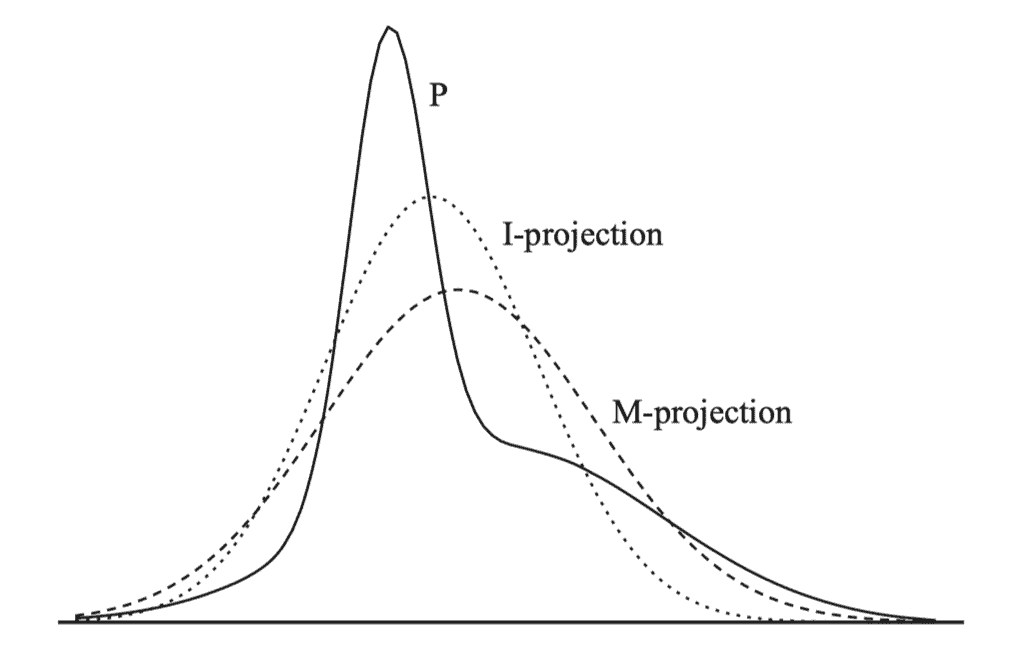
\includegraphics[width=0.5\textwidth]{Figs/a27.png}
    \caption{ Example of M- and I-projections into the family of Gaussian distributions}
    \label{fig:aod2qa}
\end{figure}
$\bullet$ \tb{Study of M-projection}

Recall that the M-projection $Q^{M}$ minimizes
\begin{align*}
\mathbb{D}(P \| Q)=-\mathbb{H}_{P}(X)+\mathbb{E}_{P}[-\ln Q(X)] .
\end{align*}
We see that, in general, we want $Q^{M}$ to have high density in regions that are probable according to $P$, since a small $-\ln Q(X)$ in these regions will lead to a smaller second term. At the same time, there is a high penalty for assigning low density to regions where $P(X)$ is nonnegligible. As a consequence, although the M-projection attempts to match the main mass of $P$, its \tb{high variance is a compromise to ensure that it assigns reasonably high density to all regions that are in the support of $P$.}

\end{exma}


$\bullet$ \tb{Study of I-projection}

On the other hand, the I-projection minimizes
\begin{align*}
\mathbb{D}(Q \| P)=-\mathbb{H}_{Q}(X)+\mathbb{E}_{Q}[-\ln P(X)] .
\end{align*}
Thus, the first term incurs a penalty for low entropy, which in the case of a Gaussian $Q$ translates to a penalty on small variance. The second term, $\mathbb{E}_{Q}[-\ln P(X)]$, encodes a preference for assigning \tb{higher density to regions where $P(X)$ is large and very low density to regions where $P(X)$ is small.} Without the first term, we can minimize the second by putting all of the mass of $Q$ on the most probable point according to $P$. 
A similar phenomenon occurs in discrete distributions.
\begin{exma}
Now consider the projection of a distribution $P(A, B)$ onto the family of factored distributions $Q(A, B)=Q(A) Q(B)$. Suppose $P(A, B)$ is the following distribution:
\begin{align*}
\begin{aligned}
&P\left(a^{0}, b^{0}\right)=0.45 \\
&P\left(a^{0}, b^{1}\right)=0.05 \\
&P\left(a^{1}, b^{0}\right)=0.05 \\
&P\left(a^{1}, b^{1}\right)=0.45
\end{aligned}
\end{align*}

M-projection of this distribution is 
the uniform distribution:
\begin{align*}
\begin{aligned}
Q^{M}\left(a^{0}, b^{0}\right) &=0.5 * 0.5=0.25 \\
Q^{M}\left(a^{0}, b^{1}\right) &=0.5 * 0.5=0.25 \\
Q^{M}\left(a^{1}, b^{0}\right) &=0.5 * 0.5=0.25 \\
Q^{M}\left(a^{1}, b^{1}\right) &=0.5 * 0.5=0.25
\end{aligned}
\end{align*}
In contrast, the I-projection focuses on one of the two "modes" of the distribution, either when both $A$ and $B$ are true or when both are false. Since the distribution is symmetric about these modes, there are two I-projections. One of them is
\begin{align*}
\begin{aligned}
Q^{I}\left(a^{0}, b^{0}\right) &=0.25 * 0.25=0.0625 \\
Q^{I}\left(a^{0}, b^{1}\right) &=0.25 * 0.75=0.1875 \\
Q^{I}\left(a^{1}, b^{0}\right) &=0.75 * 0.25=0.1875 \\
Q^{I}\left(a^{1}, b^{1}\right) &=0.75 * 0.75=0.5625
\end{aligned}
\end{align*}
The second I-projection is symmetric around the opposite mode $a^{0}, b^{0}$.
\end{exma}
\begin{rema}
In this case, this behavior results in a uniform distribution for the M-projection, whereas the I-projection places most of the probability mass on one of the two assignments where $P$ has high probability.
\end{rema}


$\bullet$ \tb{Summary:}

\begin{itemize}
    \item The M-projection attempts to give all assignments reasonably high probability, whereas 
    \item the I-projection attempts to focus on high-probability assignments in $P$ while maintaining a reasonable entropy. 
\end{itemize}

\subsubsection{M-Projections to Exponential Family}
$\bullet$ \tb{Special Case:}
\begin{lema}\label{lem:mdradf}
 Let $P$ be a distribution over $X_{1}, \ldots, X_{n}$, and let $\mathcal{Q}$ be the family of distributions consistent with $\mathcal{G}_{\emptyset}$, the empty graph (no edge). Then
\begin{align*}
Q^{M}=\arg \min _{Q \models \mathcal{G}_{\emptyset}} \mathbb{D}(P \| Q)
\end{align*}
is the distribution:
\begin{align*}
Q^{M}\left(X_{1}, \ldots, X_{n}\right)=P\left(X_{1}\right) P\left(X_{2}\right) \cdots P\left(X_{n}\right)
\end{align*}
\end{lema}
\begin{rema}
Hence, the M-projection of $P$ onto the factored distribution is simply the product of marginals of $P$.
%For  the family $\mathcal{Q}$ the vector of sufficient statistics is  simply counting, for each variable $X_{i}$, the number of occurrences of each of its values. The marginal distributions over the $X_{i}$ 's are simply the expectations, relative to $P$, of these sufficient statistics. We see that, by selecting $Q$ to match these expectations, we obtain the M-projection.
\end{rema}
\begin{proof}
Consider a distribution $Q \models \mathcal{G}_{\emptyset}$. Since $Q$ factorizes, we can rewrite $\mathbb{D}(P \| Q)$ :
\begin{align*}
\begin{aligned}
\mathbb{D}(P \| Q) &=\mathbb{E}_{P}\left[\ln P\left(X_{1}, \ldots, X_{n}\right)-\ln Q\left(X_{1}, \ldots, X_{n}\right)\right] \\
&=\mathbb{E}_{P}\left[\ln P\left(X_{1}, \ldots, X_{n}\right)\right]-\sum_{i} \mathbb{E}_{P}\left[\ln Q\left(X_{i}\right)\right] \\
&=\mathbb{E}_{P}\left[\ln \frac{P\left(X_{1}, \ldots, X_{n}\right)}{P\left(X_{1}\right) \cdots P\left(X_{n}\right)}\right]+\sum_{i} \mathbb{E}_{P}\left[\ln \frac{P\left(X_{i}\right)}{Q\left(X_{i}\right)}\right] \\
&=\mathbb{D}\left(P \| Q^{M}\right)+\sum_{i} \mathbb{D}\left(P\left(X_{i}\right) \| Q\left(X_{i}\right)\right) \\
& \geq \mathbb{D}\left(P \| Q^{M}\right)
\end{aligned}
\end{align*}
The last step relies on the nonnegativity of the relative entropy. We conclude that $\mathbb{D}(P \| Q) \geq$ $\mathbb{D}\left(P \| Q^{M}\right)$ with equality only if $Q\left(X_{i}\right)=P\left(X_{i}\right)$ for all $i$. That is, only when $Q=Q^{M}$.
\end{proof}

$\bullet$ \tb{General Case:} 

\begin{thma}\label{thm:jdfkjsafads}
Let $P$ be a distribution over $\mathcal{X}$, and let $\mathcal{Q}$ be an exponential family defined by the functions $\tau(\xi)$ and $\mathrm{t}(\boldsymbol{\theta})$. If there is a set of parameters $\boldsymbol{\theta}$ such that $\mathbb{E}_{Q_{\boldsymbol{\theta}}}[\tau(\mathcal{X})]=\mathbb{E}_{P}[\tau(\mathcal{X})]$, then the M-projection of $P$ is $Q_{\boldsymbol{\theta}}$.
\end{thma}
\begin{rema}\bfs{explanation}
The characterization of a distribution $P$ that is relevant to computing its M-projection into $\mathcal{Q}$ is \tb{expectation of the sufficient statistic function} of $\mathcal{Q}$ w.r.t. $P$. Thus, instead of describing a distribution in the family $\calQ$ by the set of parameters, \tb{we can describe it in terms of the expected sufficient statistics.}
\end{rema}
\begin{rema}\bfs{explanation for special case}
Consider the discrete case, the sufficient statistics in \cref{lem:mdradf} can be viewed as indicator function of each $X_i$'s values. The expectations are then the marginal probabilities.
\end{rema}
\begin{proof}
Suppose that $\mathbb{E}_{P}[\tau(\mathcal{X})]=\mathbb{E}_{Q_{\boldsymbol{\theta}}}[\tau(\mathcal{X})]$, and let $\boldsymbol{\theta}^{\prime}$ be some set of parameters. Then,
\begin{align*}
\begin{aligned}
\mathbb{D}\left(P \| Q_{\boldsymbol{\theta}^{\prime}}\right)-\mathbb{D}\left(P \| Q_{\boldsymbol{\theta}}\right)=&-\mathbb{H}_{P}(\mathcal{X})-\left\langle\mathbb{E}_{P}[\tau(\mathcal{X})], \mathrm{t}\left(\boldsymbol{\theta}^{\prime}\right)\right\rangle+\ln Z\left(\boldsymbol{\theta}^{\prime}\right) \\
&+\mathbb{H}_{P}(\mathcal{X})+\left\langle\mathbb{E}_{P}[\tau(\mathcal{X})], \mathrm{t}(\boldsymbol{\theta})\right\rangle-\ln Z(\boldsymbol{\theta}) \\
=&\left\langle\mathbb{E}_{P}[\tau(\mathcal{X})], \mathrm{t}(\boldsymbol{\theta})-\mathrm{t}\left(\boldsymbol{\theta}^{\prime}\right)\right\rangle-\ln \frac{Z(\boldsymbol{\theta})}{Z\left(\boldsymbol{\theta}^{\prime}\right)} \\
=&\left\langle\mathbb{E}_{Q_{\boldsymbol{\theta}}}[\tau(\mathcal{X})], \mathrm{t}(\boldsymbol{\theta})-\mathrm{t}\left(\boldsymbol{\theta}^{\prime}\right)\right\rangle-\ln \frac{Z(\boldsymbol{\theta})}{Z\left(\boldsymbol{\theta}^{\prime}\right)} \\
=& \mathbb{D}\left(Q_{\boldsymbol{\theta}} \| Q_{\boldsymbol{\theta}^{\prime}}\right) \geq 0
\end{aligned}
\end{align*}
We conclude that the M-projection of $P$ is $Q_{\theta}$.
\end{proof}


\begin{defa}\bfs{Expected Sufficient Statistics}
We define a mapping from legal parameters in $\Theta$ to vectors of sufficient statistics
\begin{align*}
\mathrm{ess}(\boldsymbol{\theta})=\mathbb{E}_{Q_{\theta}}[\tau(\mathcal{X})]
\end{align*}
\end{defa} 

\cref{thm:jdfkjsafads} shows that if $\mathbb{E}_{P}[\tau(\mathcal{X})]$ is in the image of $\mathrm{ess}$, then the M-projection of $P$ is the distribution $Q_{\theta}$ that matches the expected sufficient statistics of $P$. In other words,
\begin{align*}
\mathbb{E}_{Q^{M}}[\tau(\mathcal{X})]=\mathbb{E}_{P}[\tau(\mathcal{X})]
\end{align*}
This result explains why M-projection is also referred to as \tb{moment matching}.  We illustrate these concepts in figure \cref{fig:aod2qa}.

 \begin{figure}[H]
    \centering
    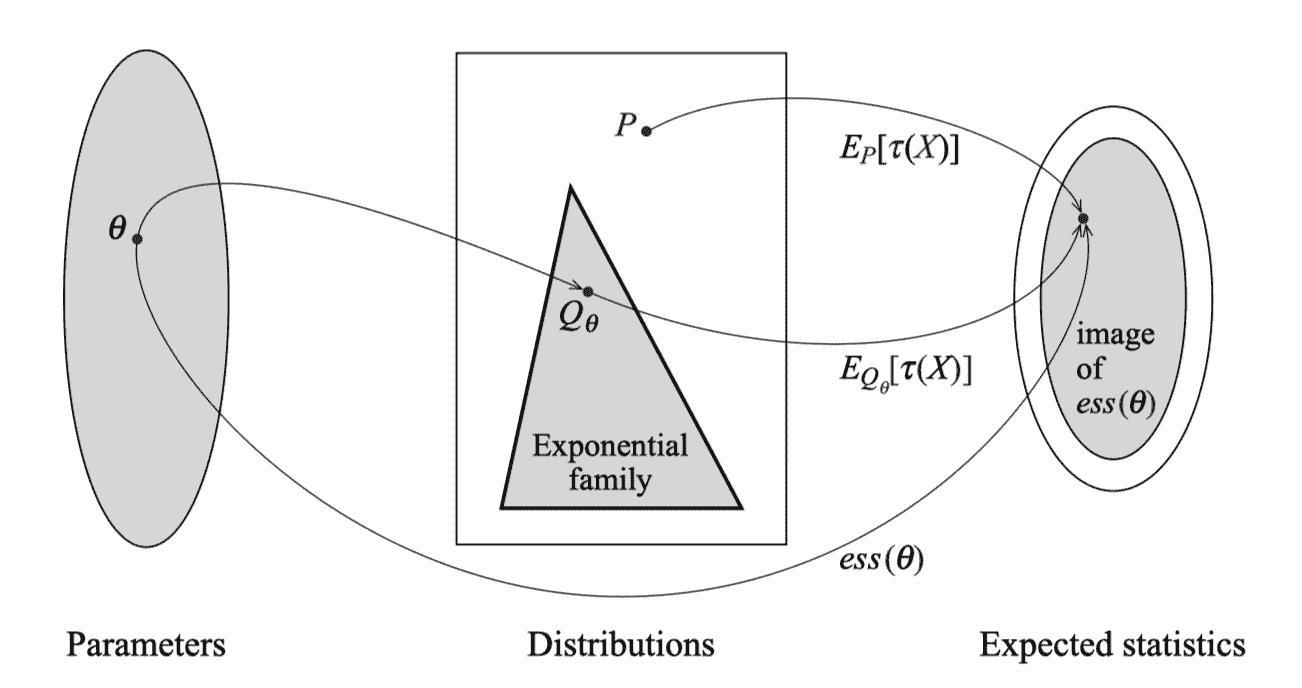
\includegraphics[width=0.8\textwidth]{Figs/a28.png}
    \caption{Illustration of the relations between parameters, distributions and expected sufficient statistics. Each parameter corresponds to a distribution, which in turn corresponds to a value of the expected statistics. The function $\mathrm{ess}$ maps parameters directly to expected statistics. If the expected statistics of $P$ and $Q_{\theta}$ match, then $Q_{\theta}$ is the M-projection of $P$.}
    \label{fig:aod2qa}
\end{figure}



From \cref{thm:jdfkjsafads}, we  obtain a general characterization of the M-projection function $\mathrm{M-project}(s)$, which maps a vector of \tb{expected sufficient statistics to a parameter vector}:
\begin{cora}
 Let $\boldsymbol{s}$ be a vector. If $s \in \mathrm{image}(\mathrm{ess})$ and $\mathrm{ess}$ is \tb{invertible}, then
\begin{align*}
\mathrm{M-project}(\boldsymbol{s})=\mathrm{ess}^{-1}(\boldsymbol{s}).
\end{align*}
\end{cora}
\begin{rema}That is, the parameters of the M-projection of $P$ are simply the inverse of the ess mapping, applied to the expected sufficient statistic vector of $P$. In many examples that we consider, the image of ess includes all possible vectors of expected sufficient statistics we might encounter. Moreover, if the parameterization is \tb{nonredundant}, then $\mathrm{ess}$  is invertible. See ``Mathematical Statistics Notes''.
\end{rema}


\paragraph{Examples}
\begin{exma}\bfs{Gaussian Distributions}
Consider the exponential family of Gaussian distributions. Recall that the sufficient statistics function for this family is $\tau(x)=\left\langle x, x^{2}\right\rangle$. Given parameters $\boldsymbol{\theta}=\left\langle\mu, \sigma^{2}\right\rangle$, the expected value of $\tau$ is
\begin{align*}
\mathrm{ess}\left(\left\langle\mu, \sigma^{2}\right\rangle\right)=\mathbb{E}_{Q_{\left\langle\mu, \sigma^{2}\right\rangle}}[\tau(X)]=\left\langle\mu, \sigma^{2}+\mu^{2}\right\rangle .
\end{align*}
It is not difficult to show that, for any distribution $P, \mathbb{E}_{P}[\tau(X)]$ must be in the image of this function. Thus, for any choice of $P$, we can apply \cref{thm:jdfkjsafads}.
Finally, we can easily invert this function:
\begin{align*}
\mathrm{M-project}\left(\left\langle s_{1}, s_{2}\right\rangle\right)=e s s^{-1}\left(\left\langle s_{1}, s_{2}\right\rangle\right)=\left\langle s_{1}, s_{2}-s_{1}^{2}\right\rangle .
\end{align*}
Recall that $s_{1}=\mathbb{E}_{P}[X]$ and $s_{2}=\mathbb{E}_{P}\left[X^{2}\right]$. Thus, the estimated parameters are the mean and variance of $X$ according to $P$, as we would expect.
\end{exma}
\begin{rema}
This example shows that the "naive" choice of Gaussian distribution, obtained by matching the mean and variance of a variable $X$, provides the best Gaussian approximation (in the M-projection sense) to a non-Gaussian distribution over $X$.
\end{rema}

\begin{exma}\bfs{Chain Network}
We now consider a more complex example of M-projection onto a chain network. Suppose we have a distribution $P$ over variables $X_{1}, \ldots, X_{n}$, and want to project it onto the family of distributions $Q$ of the distributions that are consistent with the network structure $X_{1} \rightarrow X_{2} \rightarrow \cdots \rightarrow X_{n}$.

$\diamond$ What are the \tb{sufficient statistics} for this network? 

Based on our previous discussion, we see that each conditional distribution $Q\left(X_{i+1} \mid X_{i}\right)$ requires a \tb{statistic} of the form
\begin{align*}
\tau_{x_{i}, x_{i+1}}(\xi)=\indicate{X_{i}=x_{i}, X_{i+1}=x_{i+1}}\quad \forall\left\langle x_{i}, x_{i+1}\right\rangle \in \mathrm{Val}\left(X_{i}\right) \times \mathrm{Val}\left(X_{i+1}\right) .
\end{align*}
These statistics are sufficient but are redundant. To see this, note that the "marginal statistics" must agree. That is,
\begin{align}
\sum_{x_{i}} \tau_{x_{i}, x_{i+1}}(\xi)=\sum_{x_{i+2}} \tau_{x_{i+1}, x_{i+2}}(\xi) \quad  \forall x_{i+1} \in \mathrm{Val}\left(X_{i+1}\right)\label{eq:ujnfa}
\end{align}

$\diamond$ \tb{Expectation of sufficient statistics}:

Although this representation is redundant, we can still apply the mechanisms discussed earlier and consider the function $\mathrm{ess}$ that maps parameters of such a network to the sufficient statistics. The \tb{expectation of an indicator function is the marginal probability} of that event, so that
\begin{align*}
\mathbb{E}_{Q_{\boldsymbol{\theta}}}\left[\tau_{x_{i}, x_{i+1}}(\mathcal{X})\right]=Q_{\boldsymbol{\theta}}\left(x_{i}, x_{i+1}\right) .
\end{align*}
Thus, the function $\mathrm{ess}$ simply maps from $\boldsymbol{\theta}$ to the pairwise marginals of consecutive variables in $Q_{\theta}$. Because these are pairwise marginals of an actual distribution, it follows that these sufficient statistics satisfy the consistency constraints of \cref{eq:ujnfa}.

$\diamond$ How do we invert this function? 

Given the statistics from $P$, we want to find a distribution $Q$ that matches them. We start building $Q$ along the structure of the chain. We choose $Q\left(X_{1}\right)$ and $Q\left(X_{2} \mid X_{1}\right)$ so that $Q\left(x_{1}, x_{2}\right)=\boldsymbol{E}_{P}\left[\tau_{x_{1}, x_{2}}(\mathcal{X})\right]=P\left(x_{1}, x_{2}\right)$. In fact, there is a unique choice that satisfies this equality, where $Q\left(X_{1}, X_{2}\right)=P\left(X_{1}, X_{2}\right)$. This choice implies that the marginal distribution $Q\left(X_{2}\right)$ matches the marginal distribution $P\left(X_{2}\right) .$ Now, consider our choice of $Q\left(X_{3} \mid X_{2}\right)$. We need to ensure that
\begin{align*}
Q\left(x_{3}, x_{2}\right)=\boldsymbol{E}_{P}\left[\tau_{x_{2}, x_{3}}(\mathcal{X})\right]=P\left(x_{2}, x_{3}\right) .
\end{align*}
We note that, because $Q\left(x_{3}, x_{2}\right)=Q\left(x_{3} \mid x_{2}\right) Q\left(x_{2}\right)=Q\left(x_{3} \mid x_{2}\right) P\left(x_{2}\right)$, we can achieve this equality by setting $Q\left(x_{3} \mid x_{2}\right)=P\left(x_{3} \mid x_{2}\right)$. Moreover, this implies that $Q\left(x_{3}\right)=P\left(x_{3}\right)$. We can continue this construction \tb{recursively} to set
\begin{align*}
Q\left(x_{i+1} \mid x_{i}\right)=P\left(x_{i+1} \mid x_{i}\right) .
\end{align*}

Using the preceding argument, \tb{we can show that this choice will match the sufficient statistics of $P$. This suffices to show that this $Q$ is the M-projection of P.}
\end{exma}
\begin{rema}
Note that, although this choice of $Q$ coincides with $P$ on pairwise marginals of consecutive variables, it does not necessarily agree with $P$ on other marginals.
\end{rema}
So far, all of our examples have had the characteristic that the vector of expected sufficient statistics for a distribution $P$ is always in the image of $\mathrm{ess}$, thus, our task has only been to invert $\mathrm{ess}$. Unfortunately, there are examples where \tb{not every vector of expected sufficient statistics can also be derived from a distribution in our exponential family.}
\begin{exma}
Consider again the family $\mathcal{Q}$ from \cref{ex:mndfafda}, of distributions parameterized using network structure $A \rightarrow C \leftarrow B$, with binary variables $A, B, C$. We can show that the sufficient statistics for this distribution are indicators for all the joint assignments to $A, B$, and $C$ except one. That is,
\begin{align*}
\begin{aligned}
\tau(A, B, C)=\langle& \indicate{A=a^{1}, B=b^{1}, C=c^{1}}, \\
& \indicate{A=a^{0}, B=b^{1}, C=c^{1}}, \\
& \indicate{A=a^{1}, B=b^{0}, C=c^{1}}, \\
& \indicate{A=a^{1}, B=b^{1}, C=c^{0}}, \\
& \indicate{A=a^{1}, B=b^{0}, C=c^{0}}, \\
& \indicate{A=a^{0}, B=b^{1}, C=c^{0}}, \\
&\left.\indicate{A=a^{0}, B=b^{0}, C=c^{1}}\right\rangle .
\end{aligned}
\end{align*}
If we look at the expected value of these statistics given some member of the family, we have that, since $A$ and $B$ are independent in $Q_{\theta}, Q_{\theta}\left(a^{1}, b^{1}\right)=Q_{\theta}\left(a^{1}\right) Q_{\theta}\left(b^{1}\right)$. Thus, the expected statistics should satisfy
\begin{align*}
\begin{gathered}
\mathbb{E}_{Q_{\theta}}\left[\indicate{A=a^{1}, B=b^{1}, C=c^{1}}\right]+\mathbb{E}_{Q_{\theta}}\left[\indicate{A=a^{1}, B=b^{1}, C=c^{0}}\right]= \\
\left(\mathbb{E}_{Q_{\theta}}\left[\indicate{A=a^{1}, B=b^{1}, C=c^{1}}\right]+\mathbb{E}_{Q_{\theta}}\left[\indicate{A=a^{1}, B=b^{1}, C=c^{0}}\right]\right. \\
\left.+\mathbb{E}_{Q_{\theta}}\left[\indicate{A=a^{1}, B=b^{0}, C=c^{1}}\right]+\mathbb{E}_{Q_{\theta}}\left[\indicate{A=a^{1}, B=b^{0}, C=c^{0}}\right]\right) \\
\left(\mathbb{E}_{Q_{\theta}}\left[\indicate{A=a^{1}, B=b^{1}, C=c^{1}}\right]+\mathbb{E}_{Q_{\theta}}\left[\indicate{A=a^{1}, B=b^{1}, C=c^{0}}\right]\right. \\
\left.+\mathbb{E}_{Q_{\theta}}\left[\indicate{A=a^{0}, B=b^{1}, C=c^{1}}\right]+\mathbb{E}_{Q_{\theta}}\left[\indicate{A=a^{0}, B=b^{1}, C=c^{0}}\right]\right)
\end{gathered}
\end{align*}
This constraint is not typically satisfied by the expected statistics from a general distribution $P$ we might consider projecting. Thus, in this case, \tb{there are expected statistics vectors that do not fall within the image of $\mathrm{ess}$.}
\end{exma}


In such cases, and in Bayesian networks in general, the projection procedure is more complex than inverting the $\mathrm{ess}$ function. Nevertheless, we can show that the projection operation still has an analytic solution.
\begin{thma}
Let $P$ be a distribution over $X_{1}, \ldots, X_{n}$, and let $\mathcal{G}$ be a Bayesian network structure. Then the M-projection $Q^{M}$ is:
\begin{align*}
Q^{M}\left(X_{1}, \ldots, X_{n}\right)=\prod_{i} P\left(X_{i} \mid \mathrm{Pa}_{X_{i}}^{\mathcal{G}}\right)
\end{align*}
\end{thma}
\begin{proof}
Because the mapping ess for Bayesian networks is not invertible, the proof of this result does not build on \cref{thm:jdfkjsafads} but rather directly on \cref{thm:jadffq}.
\end{proof}
\subsubsection{I-Projections}
What about I-projections? Recall that
\begin{align*}
\boldsymbol{D}(Q \| P)=-\boldsymbol{H}_{Q}(\mathcal{X})-\boldsymbol{E}_{Q}[\ln P(\mathcal{X})] .
\end{align*}
If $Q$ is in some exponential family, we can use the derivation of \cref{thm:entropy_exp} to simplify the entropy term. However, the exponential form of $Q$ does not provide insights into the second term. When dealing with the I-projection of a general distribution $P$, we are left without further simplifications. However, if the distribution $P$ has some structure, we might be able to simplify $\boldsymbol{E}_{Q}[\ln P(\mathcal{X})]$ into simpler terms, although the projection problem is still a nontrivial one.
\bibliographystyle{IEEEtran}
\bibliography{IEEEabrv,StringDefinitions,adv_dnn}
\end{document}




